\section{Reduction strategies}
\label{sec:redstrat}
Reductions in the context of the lambda calculus are a small set of well-defined rules for rewriting such that a program is proved or evaluated.
The techniques required to correctly prove and evaluate a program are a bit more complicated than the SKI calculus but are rewarding in flexibility and performance.
Throughout this section we will explore what difficulties lie within proving and evaluating the untyped lambda calculus via reduction strategies.
The first section will interest itself with the semantics of proving the untyped lambda calculus, whilst the second will implement a machine capable of evaluating a result.

\subsection{Symbols and notation}
In this section, expressions will be written in a different typesetting since some expressions and symbols mean something different than in other sections.
For instance \texttt{x $\rightarrow$ y} means the evaluation of \texttt{x} results in \texttt{y}, while $x \rightarrow y$ means the type of a function that takes a value of type $x$ and returns a value of type $y$.

The following sections will have many variables with different meaning, therefore symbols are constrained to certain types of values as described in \autoref{eq:redstrat:sym}.
\begin{align}
	\texttt{x, y, z, f, v, $\gamma$ }      & \texttt{:= Var}\label{eq:redstrat:sym} \\
	\texttt{e, p, l, o }                   & \texttt{:= Exp}\tag*{}                 \\
	\texttt{$\Gamma$, $\Sigma$, $\Theta$ } & \texttt{:= Heap}\tag*{}                \\
	\texttt{E }                            & \texttt{:= Environment}\tag*{}
\end{align}
\texttt{Exp} is any expression, expressible in both untyped lambda calculus and future extensions.


\subsection{The abstract evaluation model}\label{sec:abstractmachine}
The environment is a set of substitutions, that is, a set of variable names to their value denoted \texttt{\{x $\mapsto$ $\lambda$y.y\}} meaning ``the value of variable \texttt{x} is \texttt{$\lambda$y.y}''.
\begin{remark}
	In the section regarding the semantics of reduction strategies, environments will exist as singleton sets, named \textit{substitutions}.
\end{remark}
%Substitutions mappings can be combined $S \cup \Sigma$, if a variable name occurs in both $S$ and $\Sigma$ then the variable in the rightmost mapping is chosen ($\Sigma$).
\begin{align}
	\texttt{\{x $\mapsto$ y\}x = y}\label{eq:subsem}
\end{align}
Substitutions are performed like shown in \autoref{eq:subsem}, which states ``x is substituted by y''.
%In $(\lambda f . \lambda x . \lambda y. \texttt{ let } a = f x \texttt{ in } a + y)(\lambda y . y) \,\, 10 \,\, 20$ when evaluating $f x$ where the substitution are $[f \mapsto \lambda y . y, x \mapsto 10, y \mapsto 20]$ there must be taken great care that $x$ is mapped to $y$ in $\lambda y . y$.

Evaluation strategies (\autoref{sec:es}) are a core part of the reduction strategy since the choice of evaluation strategy determines the order in which terms are evaluated.
%A \textit{redex} is a reducible expression in the context of some set of reduction rules.
%The two interesting evaluation orders are \textit{applicative order} and \textit{normal order}~\cite{sestoft2002demonstrating}.
%The most interesting evaluation order is 
%Applicative order specifies that the parameters of some application should always be evaluated first, e.g. call by value.
%Normal order specifies that the leftmost outermost term should be evaluated first which yields the call by name strategy.
The order of evaluation decides the evaluation strategy and also the final form of expressions~\cite{sestoft2002demonstrating}.
Before delving into more complicated evaluation strategies such as call by need, call by name will be considered.

A reduction strategy would involve substituting variables, once they are applied.
When evaluating a term such as \texttt{($\lambda$x.x) y}, \texttt{x} must be substituted by \texttt{y} such that the expression then becomes \texttt{x} with the substitution \texttt{\{x $\mapsto$ y\}} and finally becomes \texttt{y} after the substitution has occurred.
\begin{figure}[ht]
	\begin{mdframed}[style=bigbox]
		\vspace*{0.49cm}
		\begin{subfigure}[b]{0.48\textwidth}
			\begin{prooftree}
				\AxiomC{}
				\RightLabel{Abs}
				\UnaryInfC{\texttt{($\lambda$x.e) $\rightarrow$ ($\lambda$x.e)}}
			\end{prooftree}
			\caption{}
			\label{eq:simpleabs}
		\end{subfigure}
		\begin{subfigure}[b]{0.48\textwidth}
			\vspace*{0.4cm}
			\begin{prooftree}
				\AxiomC{}
				%\AxiomC{$S \alpha x \not\equiv \alpha x$}
				\RightLabel{Var}
				\UnaryInfC{\texttt{x $\rightarrow$ x}}
			\end{prooftree}
			\caption{}
			\label{eq:simplevar}
		\end{subfigure}
		\begin{subfigure}[b]{1\textwidth}
			\vspace*{0.4cm}
			\begin{prooftree}
				\AxiomC{\texttt{\{x $\mapsto$ e\} p $\rightarrow$ l}}
				\RightLabel{Let}
				\UnaryInfC{\texttt{let x = e in p $\rightarrow$ l}}
			\end{prooftree}
			\caption{}
			\label{fig:simplelet}
		\end{subfigure}
		\begin{subfigure}[b]{1\textwidth}
			\vspace*{0.4cm}
			\begin{prooftree}
				\AxiomC{\texttt{l $\rightarrow$ ($\lambda$x.e)}}
				\AxiomC{\texttt{\{x $\mapsto$ p\} e $\rightarrow$ o}}
				\RightLabel{App}
				\BinaryInfC{\texttt{l p $\rightarrow$ o}}
			\end{prooftree}
			\caption{A simple application rule}
			\label{fig:simpleapp}
		\end{subfigure}
	\end{mdframed}
	\caption{Simple call by name lambda calculus}
	\label{fig:scbn}
\end{figure}
The rules in \autoref{fig:scbn} display a simple set of rules for proving call by name lambda calculus programs.
\begin{itemize}
	\item The Abs and Var rules (\autoref{eq:simpleabs} and \autoref{eq:simplevar}) are rules which act as terminal cases of a proof.
	      Abs and Var both state that if either of them occur then the expression must be an axiom by their identity.
	\item The App rule (\autoref{fig:simpleapp}) states that ``\texttt{l p} can be proved to evaluate to \texttt{o} if \texttt{l} can be proved to be \texttt{($\lambda$x.e)} and \texttt{e} can be proved to evaluate to \texttt{o}, where \texttt{x} has been replaced by \texttt{p} in \texttt{e}''.
	\item The Let rule has the same function as the App rule, but will have an important role in a more refined version of the semantics.
\end{itemize}
We must introduce rules for how substitutions should act upon encountering lambda calculus terms (\autoref{eq:subsem}).
\begin{align}
	 & \texttt{\{x $\mapsto$ e\}x = e} \label{eq:subsem}                \\
	 & \texttt{\{x $\mapsto$ e\}p = p}  \tag*{}                         \\
	 & \texttt{E(l p) = (El)(Ep)} \tag*{}                               \\
	 & \texttt{E($\lambda$x.e) = ($\lambda$x.Ee) } \label{eq:subsemrem} %\\
\end{align}

\subsubsection{Ambiguous programs}
\begin{align}
	\texttt{($\lambda$x.($\lambda$x.x) 0) 1} \label{eq:ambgprog}
\end{align}
Proving \autoref{eq:ambgprog} under the rules in \autoref{eq:subsem} yields a case for more thorough substitution rules.
By inspection one can determine that a simple program like \autoref{eq:ambgprog} yields the symbol \texttt{0}, but alas this is not the case.
The first step to prove \autoref{eq:ambgprog} is to apply the App rule, which prompts the application of the Abs rule on the left side for \texttt{f}, such that the expression to prove now becomes the lambda abstraction with \texttt{x} replaced by \texttt{1} (\autoref{eq:ambgprog2}).
\begin{align}
	\texttt{($\lambda$x.1) 0} \label{eq:ambgprog2}
\end{align}
Clearly \autoref{eq:ambgprog2} changed the meaning of the program.
If we continue the proof which states that the program in \autoref{eq:ambgprog2} should evaluate to the symbol \texttt{0}, we would not be in luck.
Clearly this system is not sound, thus requires some further refinement.
%\begin{figure}
%\begin{lstlisting}[language=ML,caption={Program with variable ambiguity},label={lst:varambg},mathescape=true]
%fun f x =
%fun g x = x;
%g (x + x);
%f 2;
%\end{lstlisting}
%\end{figure}
%Evaluating \autoref{lst:varambg} under the rules in \autoref{eq:subsem} yields a case for more thorough substitution rules.
%Using the App rule (\autoref{fig:simpleapp}) and applying substitutions as defined in (\autoref{eq:subsem}), yields the program in \autoref{lst:varambg2}.
%\begin{lstlisting}[language=ML,caption={Program with variable ambiguity after one reduction pass},label={lst:varambg2},mathescape=true]
%fun g x = 2;
%g (2 + 2);
%\end{lstlisting}
%Which eventually evaluates to \texttt{2}, which clearly is not the intended result.
Removing the rule \autoref{eq:subsemrem} and adding the two rules in \autoref{eq:subsemfixed} solves this type.
\begin{align}
	 & \texttt{E($\lambda$x.e) = ($\lambda$x.Ee)}                                & \texttt{(x $\mapsto$ p) $\notin$ S} \label{eq:subsemfixed} \\
	 & \texttt{E($\lambda$x.e) = ($\lambda$x.(E$\backslash$\{x $\mapsto$ p\})e)} & \texttt{(x $\mapsto$ p) $\in$ S} \tag*{}
\end{align}
This is a simple instance of variable ambiguity, a more problematic variant exists which goes by the name of variable capture.
This evaluation model is indeed powerful enough to evaluate \textbf{most} call by name lambda calculus programs.
\begin{exmp}
	With the aforementioned rules, programs can now be proved.
	Note that the Substitution rule in \autoref{fig:rules:exmp:sol} is simply the substitution semantics from \autoref{eq:subsemfixed} made clearer.
	Let the program in \autoref{eq:exmp:subrules}, where \texttt{0} is a symbol of any type, be subject to the rules in \autoref{fig:scbn}, which solves to \autoref{fig:rules:exmp:sol}.
	\begin{align}
		\texttt{(($\lambda$f.$\lambda$x.f x) ($\lambda$x.x)) 0}\label{eq:exmp:subrules}
	\end{align}
	\begin{figure}[ht]
		\begin{mdframed}
			\vspace*{0.49cm}
			\begin{subfigure}[b]{1\textwidth}
				\begin{prooftree}
					\AxiomC{}
					\LeftLabel{Abs}
					\UnaryInfC{\texttt{($\lambda$x.($\lambda$x.x) x) $\rightarrow$ ($\lambda$x.($\lambda$x.x) x)}}
					\LeftLabel{Substitution}
					\UnaryInfC{\texttt{\{f $\mapsto$ ($\lambda$x.x)\}($\lambda$x.f x) $\rightarrow$ ($\lambda$x.($\lambda$x.x) x)}}
				\end{prooftree}
				\caption{}
				\label{fig:rules:exmp:left:right}
			\end{subfigure}
			\vspace*{0.49cm}
			\begin{subfigure}[b]{1\textwidth}
				\begin{prooftree}
					\AxiomC{}
					\LeftLabel{Abs}
					\UnaryInfC{\texttt{($\lambda$f.$\lambda$x.f x) $\rightarrow$ ($\lambda$f.$\lambda$x.f x)}}
					\AxiomC{\autoref{fig:rules:exmp:left:right}}
					\LeftLabel{App}
					\BinaryInfC{\texttt{($\lambda$f.$\lambda$x.f x) ($\lambda$x.x) $\rightarrow$ ($\lambda$x.($\lambda$x.x) x)}}
				\end{prooftree}
				\caption{}
				\label{fig:rules:exmp:left}
			\end{subfigure}
			\vspace*{0.49cm}
			\begin{subfigure}[b]{1\textwidth}
				\begin{prooftree}
					\AxiomC{}
					\LeftLabel{Abs}
					\UnaryInfC{\texttt{($\lambda$x.x) $\rightarrow$ ($\lambda$x.x)}}
					\AxiomC{}
					\RightLabel{Var}
					\UnaryInfC{\texttt{0 $\rightarrow$ 0}}
					\RightLabel{Substitution}
					\UnaryInfC{\texttt{\{x $\mapsto$ 0\}x $\rightarrow$ 0}}
					\RightLabel{App}
					\BinaryInfC{\texttt{($\lambda$x.x) 0 $\rightarrow$ 0}}
					\RightLabel{Substitution}
					\UnaryInfC{\texttt{\{x $\mapsto$ 0\}($\lambda$x.x) x $\rightarrow$ 0}}
				\end{prooftree}
				\caption{}
				\label{fig:rules:exmp:right}
			\end{subfigure}
			\vspace*{0.49cm}
			\begin{subfigure}[b]{1\textwidth}
				\begin{prooftree}
					\AxiomC{\autoref{fig:rules:exmp:left}}
					\AxiomC{\autoref{fig:rules:exmp:right}}
					\LeftLabel{App}
					\BinaryInfC{\texttt{(($\lambda$f.$\lambda$x.f x) ($\lambda$x.x)) 0 $\rightarrow$ 0}}
				\end{prooftree}
			\end{subfigure}
		\end{mdframed}
		\caption{}
		\label{fig:rules:exmp:sol}
	\end{figure}
\end{exmp}

Variable capture is the basis for some practical difficulties when designing evaluation rules for the untyped lambda calculus.
Consider the following sub-program \texttt{($\lambda$x.y) g} with the following ongoing substitutions \texttt{\{x $\mapsto$ z, y $\mapsto$ x, $\dots$\}}, which contains \texttt{y} as a closure.
Substituting by the rules outlined in \autoref{eq:subsemfixed} yields \texttt{($\lambda$x.x) g} which is clearly invalid.
The invalid program result is a product of variable capture.
%The program before substitution and after should be \textit{$\alpha$-equivalent}, which they are not.
%The two program states becomes ambiguous by the ambiguity of multiple variables by the same name.
To solve ambiguity between variables with the same name, one can perform an \textit{$\alpha$-conversion}.
\begin{remark}
	Notice that if variables are renamed before program execution, recursive functions can still suffer from ambiguity since all parameters for that function can occur multiple times.
\end{remark}
\subsubsection{$\alpha$-conversions} \label{sec:alpha}
%An $\alpha$-conversion mapping can occur as the substitution mapping, that is \texttt{\{x $\mapsto$ $\gamma_1$, y $\mapsto$ $\gamma_2$\}}; $\alpha$-conversions are philosophical constructs more than materialized mappings.
An $\alpha$-conversion is a renaming operation which does not modify the meaning of the expression.
$\alpha$-conversions can be written similar to substitutions, for instance renaming \texttt{x} to $\gamma$ appears as \texttt{\{x $\mapsto$ $\gamma$\}}.
$\alpha$-conversions guarantee what is called \textit{$\alpha$-equivalence} which is the notion of semantic equivalence.
For instance \texttt{$\lambda$x.x} is $\alpha$-equivalent with \texttt{$\lambda\gamma.\gamma$} since both expressions are semantically equivalent.
%$\alpha$-conversions solve some critical problems such as closures and recursion when evaluating the lambda calculus.
%$\alpha$-conversions should also be non-destructive but still be context aware such that when leaving an abstraction the remaining substitution mapping is a superset of the substitution mapping when entering.
%More formally if \texttt{S, e $\rightarrow$ $\Sigma$, e'} then $\{x \,\,|\,\, (x \mapsto y) \in S\} \subseteq \{x \,\,|\,\, (x \mapsto y) \in \Sigma\}$.
%\begin{lstlisting}[language=ML,caption={Recursive addition function},label={lst:recalpha},mathescape=true]
%let f = ($\lambda$f'.$\lambda$x.
%if (x = 0) x else f' f' ((x - 1) + (x - 1))) in
%f f 10
%\end{lstlisting}
%A strong guarantee that can be made by tuning the evaluation strategy which is particularly useful for $\alpha$-conversion algorithms is that \textit{any} returned value has had \textit{every} term that it contains visited.
%An algorithm for performing $\alpha$-conversions can be implemented that picks a new variable name from any infinite domain when an abstraction has had a value applied to it and replaces future encountered variables with the new one, such an algorithm only works if the guarantee of visiting every term is made.
%The algorithm should also introduce the applied value to the substitution set through the alpha converted name.
%\noindent An $\alpha$-conversion algorithm can be implemented such that when a new variable is introduced through an abstraction, a new name for the variable is given.
Let $V_1$ be the domain of variables in the program and $V_2$ be the infinite domain for variable names that satisfies $V_1 \cap V_2 = \emptyset$, such that when a new variable \texttt{x} is discovered, replace it with some $\gamma \in V_2$ and let $V_2 = V_2 \backslash \{\gamma\}$.
%For instance, let \texttt{($\lambda\gamma_1$.$\lambda\gamma_2$.if ($\gamma_2$ = 0) $\gamma_2$ else $\gamma_1$ $\gamma_1$ (($\gamma_2$ - 1) + ($\gamma_2$ - 1)))} be the $\alpha$-converted version of \texttt{f} in \autoref{lst:recalpha}.
The function \texttt{fresh} picks a fresh variable name $\gamma$ from $V_2$ and updates $V_2$ to $V_2 \backslash \{\gamma\}$.
Letting the previous example \texttt{\{y $\mapsto$ x\}($\lambda$x.y) g}, be subject to $\alpha$-conversion solves the problem of ambiguity (\texttt{\{y $\mapsto$ $\tau$\}($\lambda$x.$\tau$) g}), since \texttt{y} could be renamed to a variable introduced through \texttt{fresh}, thus no ambiguity occurs.
$\alpha$-conversions will be further explored in future refinements of \autoref{fig:scbn} in the from of renaming through the Let rule.

%\subsubsection{Eager substitutions}
%Instead of performing $\alpha$-conversions to ensure variable uniqueness, one can enhance the rules in \autoref{fig:scbn}.%one can leverage the ideas proposed in~\cite{launchbury1993natural} to implement laziness, lazy substitution, solve variable ambiguity and perform efficient garbage collection.
%To further refine the call by name evaluation semantics observe that substitutions are performed eagerly, that is, they \textit{break suspension}.
%To explore solutions to avoid eager substitutions, environments may be used.
%\begin{remark}
%When considering an arbitrarily large expression under call by name (or need), there is no guarantee that the expression will ever be evaluated, that is, a suspended expression being forced.
%Rules specify what implementations must adhere to and not anything more.
%Regardless it still remains as an interest to not break suspension.
%Breaking suspension may violate the philosophy behind call by name (and need).
%A solution could involve composing a function in compile time, which replaces all instances of a variable (by \autoref{eq:subsem} and \autoref{eq:subsemfixed}) with some parameterized value.
%Substituting expressions eagerly might compromise practical performance guarantees, even if substitution is an asymptotically constant number of operations.
%Consider substituting an expression which contains conditional branches, one branch might be a simple expression and the other might be a very large expression, consisting of many instances of the same variable.
%If the program never picks the large expression, why should it ever have any impact on performance.
%For instance, in \autoref{lst:fastslow} under call by name one would expect \texttt{fastMap} to evaluate in roughly the same time as \texttt{slowMap}.
%\begin{lstlisting}[language=ML,caption={Performance considerations in substitution},label={lst:fastslow},mathescape=true]
%fun fastMap f l =
%match l
%| Nil -> Nil;
%| Cons x xs -> Cons (f x) (map f xs);
%;
%fun slowMap f l =
%match l
%| Nil -> Nil;
%| Cons x xs -> 
%if (x == 0)
%let v = x + x + x + x + x + x; 
%Cons (f x) (map f xs);
%else
%Cons (f x) (map f xs);
%;
%;
%\end{lstlisting}
%\end{remark}
\subsubsection{The heap}
Heaps, like environments in typing (\autoref{eq:env}), define what ``state'' is required to evaluate some expression.
A heap contains mappings from variables to expressions, much like the environment which performs substitutions, except it acts like a store.
Heaps are a requirement for call by need semantics.
A simple modification to the rules in \autoref{fig:rules:env}, introduces a heap which states that that the semantics must bring a heap along.
\begin{figure}[ht]
	\begin{mdframed}[style=bigbox]
		\vspace*{0.49cm}
		\begin{subfigure}[b]{0.49\textwidth}
			\begin{prooftree}
				\AxiomC{}
				\RightLabel{Abs}
				\UnaryInfC{\texttt{$\Gamma$, ($\lambda$x.e) $\rightarrow$ $\Gamma$, ($\lambda$x.e)}}
			\end{prooftree}
			\caption{}
			\label{fig:rules:env:abs}
		\end{subfigure}
		\begin{subfigure}[b]{0.49\textwidth}
			\vspace*{0.4cm}
			\begin{prooftree}
				\AxiomC{\texttt{$\Gamma$ $\cup$ \{x $\mapsto$ e\}, p $\rightarrow$ $\Theta$, l}}
				\RightLabel{Let}
				\UnaryInfC{\texttt{$\Gamma$, let x = e in p $\rightarrow$ $\Theta$, l}}
			\end{prooftree}
			\caption{}
			\label{fig:rules:env:let}
		\end{subfigure}
		\begin{subfigure}[b]{1\textwidth}
			\vspace*{0.4cm}
			\begin{prooftree}
				\AxiomC{\texttt{$\Gamma$, l $\rightarrow$ $\Theta$, ($\lambda$x.e)}}
				\AxiomC{\texttt{$\Theta$, \{x $\mapsto$ p\}e $\rightarrow$ $\Sigma$, o}}
				\RightLabel{App}
				\BinaryInfC{\texttt{$\Gamma$, l p $\rightarrow$ $\Sigma$, o}}
			\end{prooftree}
			\caption{}
			\label{fig:rules:env:app}
		\end{subfigure}
		\begin{subfigure}[b]{1\textwidth}
			\vspace*{0.4cm}
			\begin{prooftree}
				\AxiomC{\texttt{$\Gamma$, e $\rightarrow$ $\Theta$, p}}
				\RightLabel{Var}
				\UnaryInfC{\texttt{$\Gamma$ $\cup$ \{x $\mapsto$ e\}, x $\rightarrow$ $\Theta$ $\cup$ \{x $\mapsto$ e\}, p}}
			\end{prooftree}
			\caption{}
			\label{fig:rules:env:var}
		\end{subfigure}
	\end{mdframed}
	\caption{Call by name lambda calculus with environments}
	\label{fig:rules:env}
\end{figure}
The rules in \autoref{fig:rules:env} are quite different from the rules in \autoref{fig:scbn}.
\begin{itemize}
	\item Var is no longer terminal, it now inspects the heap for a replacement value for some \texttt{x}.
	      Notice that Var now removes the mapping from the heap $\Gamma$ such that recursively defined expressions cannot occur.
	\item Let now has a role which is distinct from App.
	      Let now introduces values to the heap, but does not induce a substitution.
	\item App remains the same by eagerly substituting, but now augmented with a heap.
	\item Abs is now augmented with a heap.
\end{itemize}
The rules in \autoref{fig:rules:env} are not any more powerful that the rules in \autoref{fig:scbn}, but are a basis for lazy evaluation.

\subsubsection{Lazy evaluation}
With the revised semantics in \autoref{fig:rules:env}, lazy evaluation can now be introduced.
The basis for sharing evaluated expressions is rooted in a labelling problem~\cite{levy1988sharing}.
Before delving into a set of rules which use a labelling technique, consider that sharing can be viewed as a dependency graph of expressions.
Let \autoref{fig:dependencygraph} be a depiction of the dependency graph of \autoref{eq:xyk} under the rules in \autoref{fig:rules:env}.
\begin{align}
	 & \texttt{let k = ($\lambda$z.z) ($\lambda$f.f) in }\label{eq:xyk} \\
	 & \texttt{let x = k in }\tag*{}                                    \\
	 & \texttt{let y = k in }\tag*{}                                    \\
	 & \texttt{x + y}\tag*{}
\end{align}
\begin{figure}[ht]
	\centering
	\begin{tikzpicture}[ scale=0.8, every node/.style={scale=0.8}, node distance = 0.25cm and 0.25cm]
		\node[draw=black] (e) {\texttt{($\lambda$z.z) ($\lambda$f.f)}};

		\node[draw=black, below = of e] (k) {\texttt{k}};
		\path[->] (k) edge node[left] {} (e);

		%\node[draw=black, below left = of k] (gamma1) {$\gamma_1$};
		%\path[->] (gamma1) edge node[left] {} (k);

		\node[draw=black, below left = of k] (y) {\texttt{y}};
		\path[->] (y) edge node[left] {} (k);

		%\node[draw=black, below right = of k] (gamma2) {$\gamma_2$};
		%\path[->] (gamma2) edge node[left] {} (k);

		\node[draw=black, below right = of k] (x) {\texttt{x}};
		\path[->] (x) edge node[left] {} (k);

		\node[draw,fill=none,scale=1.3,rectangle,fit=(e)(x)(y)](fbb){};
	\end{tikzpicture}
	\caption{Expression dependencies}
	\label{fig:dependencygraph}
\end{figure}
A rule which encapsulates ``when evaluating a value for a variable, save the evaluated value for future use.'' is required to support sharing computed values.
\begin{figure}[ht]
	\begin{mdframed}
		\begin{prooftree}
			\AxiomC{\texttt{$\Gamma$, e $\rightarrow$ $\Theta$, p}}
			\RightLabel{Var}
			\UnaryInfC{\texttt{$\Gamma$ $\cup$ \{x $\mapsto$ e\}, x $\rightarrow$ $\Theta$ $\cup$ \{x $\mapsto$ p\}, p}}
		\end{prooftree}
	\end{mdframed}
	\caption{}
	\label{fig:eval:share}
\end{figure}
The rule in \autoref{fig:eval:share} replaces the Var rule, and introduces a subtle difference; when a variable reference occurs the value which the variable evaluates to is saved as the new reference.
Introducing shareable expressions through Let is in it's essence a labelling of an expression.
Evaluating \autoref{eq:xyk} under the new rules reveals that evaluating \texttt{x} forces \texttt{k} to be evaluated which then forces \texttt{($\lambda$z.z) ($\lambda$f.f)}, which becomes \texttt{($\lambda$f.f)} and is then saved as the new value of \texttt{k} and then as \texttt{x}, thus the dependency tree becomes \autoref{fig:dependencygraphv2}.
\begin{figure}[ht]
	\centering
	\begin{tikzpicture}[ scale=0.8, every node/.style={scale=0.8}, node distance = 0.25cm and 0.25cm]
		\node[draw=black] (e) {\texttt{($\lambda$f.f)}};

		\node[draw=black, below left = of e] (k) {\texttt{k}};
		\path[->] (k) edge node[left] {} (e);

		%\node[draw=black, below left = of k] (gamma1) {$\gamma_1$};
		%\path[->] (gamma1) edge node[left] {} (k);

		\node[draw=black, below left = of k] (y) {\texttt{y}};
		\path[->] (y) edge node[left] {} (k);

		%\node[draw=black, below right = of k] (gamma2) {$\gamma_2$};
		%\path[->] (gamma2) edge node[left] {} (k);

		\node[draw=black, below right = of k] (x) {\texttt{x}};
		\path[->] (x) edge node[left] {} (e);

		\node[draw,fill=none,scale=1.3,rectangle,fit=(e)(x)(y)](fbb){};
	\end{tikzpicture}
	\caption{Expression dependencies after evaluating \texttt{x}}
	\label{fig:dependencygraphv2}
\end{figure}
One consideration remains, the App rule does not promote lazy evaluation.
All non-trivial parameters must be bound to a variable by the Let rule to also allow anonymous expressions to be subject to lazy evaluation.
An algorithm for binding anonymous expressions can be found in~\cite{launchbury1993natural}.

\subsubsection{Dealing with ambiguity}
The rules so far have avoided dealing with variable ambiguity.
Notice that variable capture can only occur in the Let rule, since the Let rule is the only rule of which can introduce name bindings.
Dealing with ambiguity is a matter of ensuring that variables are distinct.
Applying the technique from \autoref{sec:alpha} properly lets us evaluate programs without ambiguity.

Consider a previous case of variable capture \autoref{eq:ambg:cap}.
\begin{align}
	\texttt{\{x $\mapsto$ z, y $\mapsto$ x, $\dots$\}($\lambda$x.y) g}\label{eq:ambg:cap}
\end{align}
None of the changes so far have any impact on the falsity of the expression.
Consider that \texttt{x} and \texttt{y} must have been bound through a Let expression.
Consider also that some variable \texttt{k} cannot be subject to variable capture if \texttt{k $\notin$ Bound($\lambda$x.e)}.
Naturally if \texttt{k} is unique, that is, it is introduced through the \texttt{fresh} function from \autoref{sec:alpha} then \texttt{k} can never occur bound.
The obvious rule from these considerations must be new Let rule defined in \autoref{fig:eval:letrename}.
\begin{figure}[ht]
	\begin{mdframed}
		\begin{prooftree}
			\AxiomC{\texttt{$\Gamma$ $\cup$ \{$\gamma$ $\mapsto$ e\}, \{x $\mapsto$ $\gamma$\}p $\rightarrow$ $\Theta$, l}}
			\AxiomC{\texttt{$\gamma$ = fresh}}
			\RightLabel{Let}
			\BinaryInfC{\texttt{$\Gamma$, let x = e in p $\rightarrow$ $\Theta$, l}}
		\end{prooftree}
	\end{mdframed}
	\caption{}
	\label{fig:eval:letrename}
\end{figure}
The correctness of \autoref{fig:eval:letrename} and the aforementioned considerations are formalised in~\cite{sestoft1997deriving}.

%For instance, consider the program in \autoref{lst:progambg} and the state after line \autoref{lst:progambg:l1} is executed in \autoref{eq:progambg2} and the remaining program in \autoref{lst:progambg2}.
%The state and remaining program is intact, but evaluating line \autoref{lst:progambg2:l1} in \autoref{lst:progambg} yields the state in \autoref{eq:progambg3} which changes the meaning of \texttt{v}.
%\begin{lstlisting}[language=ML,caption={Program which may suffer from variable ambiguity},label={lst:progambg},mathescape=true]
%let v = $\$$ (let x = 5 in ($\lambda$y.y + x)) in $\label{lst:progambg:l1}$
%let x = 0 in
%v 5
%\end{lstlisting}
%\begin{gather}
%\texttt{\{v $\mapsto$ ($\lambda$y.y + x), x $\mapsto$ 5\}}\label{eq:progambg2}
%\end{gather}
%\begin{lstlisting}[language=ML,caption={Program after evaluating \texttt{v}},label={lst:progambg2},mathescape=true]
%let x = 0 in $\label{lst:progambg2:l1}$
%v 5
%\end{lstlisting}
%\begin{gather}
%\texttt{\{v $\mapsto$ ($\lambda$y.y + x), x $\mapsto$ 0\}}\label{eq:progambg3}
%\end{gather}

%Naturally renaming can occur at the Let rule, since Let introduces new variables to the heap.
%Enhancing the Let rule with renaming by the semantics from \autoref{sec:alpha} yields a replacement for Let (\autoref{fig:eval:letrename})~\cite{sestoft1997deriving}. 
%Evaluating line \autoref{lst:progambg:l1} in \autoref{lst:progambg} now yields the state in \autoref{eq:pragambgfix} which introduces \texttt{x} as a fresh variable ($\gamma$) from the \texttt{fresh} function.
%\begin{gather}
%\texttt{\{$\sigma$ $\mapsto$ ($\lambda$y.y + $\gamma$), $\gamma$ $\mapsto$ 5\}}\label{eq:pragambgfix}
%\end{gather}

\subsubsection{Introducing useful functionality}
As the set of rules stand currently one can express numbers through church encodings.
Church encodings provide a minimal and non-invasive set of combinators which allow the encoding of numbers.
Unfortunately it is not as practical as it is minimal to church encode numbers.
For instance, to represent the number \texttt{100000} one would require \texttt{100000} invocations of some successor function.
Fortunately dwelling on the representation of numbers is an easy task once one convinces themselves that ordinary numbers and arithmetic operations are friendly.

When discovering an arithmetic operations between two expressions, they must both be forced and then the pending expression must evaluated.
Clearly this rule is not encoded into the aforementioned rules, but can be modelled easily as shown in \autoref{fig:oplusrule}.
\begin{figure}[ht]
	\begin{mdframed}[style=style1]
		\begin{subfigure}[b]{1\textwidth}
			\vspace*{0.49cm}
			\begin{prooftree}
				\AxiomC{\texttt{$\Gamma$, x $\rightarrow$ $\Theta$, n}}
				\AxiomC{\texttt{$\Theta$, y $\rightarrow$ $\Sigma$, t} $\,\,\,\,\,$ \texttt{$\oplus \in \{+,-,*,\backslash, =\}$}}
				\RightLabel{Bin op}
				\BinaryInfC{\texttt{$\Gamma$, x $\oplus$ y $\rightarrow$ $\Sigma$, (n $\oplus$ t)}}
			\end{prooftree}
		\end{subfigure}
		\begin{subfigure}[b]{1\textwidth}
			\vspace*{0.49cm}
			\begin{prooftree}
				\AxiomC{\texttt{n $\in \mathbb{Z^+}$}}
				\RightLabel{Num}
				\UnaryInfC{\texttt{$\Gamma$, n $\rightarrow$ $\Gamma$, n}}
			\end{prooftree}
		\end{subfigure}
	\end{mdframed}
	\caption{}
	\label{fig:oplusrule}
\end{figure}
Notice that \autoref{fig:oplusrule} also must accompany a Num rule which introduces integers to the system.
\begin{remark}
	Notice that the Bin op rule in \autoref{fig:oplusrule} uses \texttt{x} and \texttt{y} which are in the domain of variables, since all non-trivial expressions must be bound to fresh names through Let.
\end{remark}

\begin{exmp}
	Now that rules have been established which avoid variable ambiguity through renaming and support lazy evaluation, an example seems natural.
	An expression which requires the aforementioned properties to resolve as expected is presented in \autoref{eq:doneexmp} and proved in \autoref{fig:finproofexmp}.
	\begin{align}
		\texttt{let y = (1 + 1) in ($\lambda$x.($\lambda$y.x + y) x) y}\label{eq:doneexmp}
	\end{align}
	\begin{figure}[ht]
		\begin{mdframed}[style=bigbox]
			\begin{subfigure}[b]{1\textwidth}
				\vspace*{0.49cm}
				\begin{prooftree}
					\AxiomC{}
					\LeftLabel{Lam}
					\UnaryInfC{\texttt{\{$\gamma$ $\mapsto$ (1 + 1)\}, ($\lambda$x.($\lambda$y.x + y) x) $\rightarrow$ \{$\gamma$ $\mapsto$ (1 + 1)\},($\lambda$x.($\lambda$y.x + y) x)}}
				\end{prooftree}
				\caption{}
				\label{fig:finproofexmp:app1}
			\end{subfigure}
			\begin{subfigure}[b]{1\textwidth}
				\vspace*{0.49cm}
				\begin{prooftree}
					\AxiomC{}
					\LeftLabel{Lam}
					\UnaryInfC{\texttt{\{$\gamma$ $\mapsto$ (1 + 1)\}, ($\lambda$y.$\gamma$ + y) $\rightarrow$ \{$\gamma$ $\mapsto$ (1 + 1)\}, ($\lambda$y.$\gamma$ + y)}}
				\end{prooftree}
				\caption{}
				\label{fig:finproofexmp:app2}
			\end{subfigure}
			\begin{subfigure}[b]{1\textwidth}
				\vspace*{0.49cm}
				\begin{prooftree}
					\AxiomC{}
					\LeftLabel{Num}
					\UnaryInfC{\texttt{\{\}, 1 $\rightarrow$ \{\}, 1}}
					\AxiomC{}
					\LeftLabel{Num}
					\UnaryInfC{\texttt{\{\}, 1 $\rightarrow$ \{\}, 1}}
					\LeftLabel{Bin op}
					\BinaryInfC{\texttt{\{\}, 1 + 1 $\rightarrow$ \{\}, 2}}
					\LeftLabel{Var}
					\UnaryInfC{\texttt{\{$\gamma$ $\mapsto$ (1 + 1)\}, $\gamma$ $\rightarrow$ \{$\gamma$ $\mapsto$ 2\}, 2}}

					\AxiomC{}
					\RightLabel{Num}
					\UnaryInfC{\texttt{\{\}, 2 $\rightarrow$ \{\}, 2}}
					\RightLabel{Var}
					\UnaryInfC{\texttt{\{$\gamma$ $\mapsto$ 2\}, $\gamma$ $\rightarrow$ \{$\gamma$ $\mapsto$ 2\}, 2}}

					\LeftLabel{Bin op}
					\BinaryInfC{\texttt{\{$\gamma$ $\mapsto$ (1 + 1)\}, $\gamma$ + $\gamma$ $\rightarrow$ \{$\gamma$ $\mapsto$ 2\}, 4}}
				\end{prooftree}
				\caption{}
				\label{fig:finproofexmp:bin}
			\end{subfigure}
			\begin{subfigure}[b]{1\textwidth}
				\vspace*{0.49cm}
				\begin{prooftree}
					\AxiomC{\autoref{fig:finproofexmp:app1}}
					\AxiomC{\autoref{fig:finproofexmp:app2}}
					\AxiomC{\autoref{fig:finproofexmp:bin}}
					\LeftLabel{App}
					\BinaryInfC{\texttt{\{$\gamma$ $\mapsto$ (1 + 1)\}, ($\lambda$y.$\gamma$ + y) $\gamma$ $\rightarrow$ \{$\gamma$ $\mapsto$ 2\}, 4}}
					\LeftLabel{App}
					\BinaryInfC{\texttt{\{$\gamma$ $\mapsto$ (1 + 1)\}, ($\lambda$x.($\lambda$y.x + y) x) $\gamma$ $\rightarrow$ \{$\gamma$ $\mapsto$ 2\}, 4}}
					\LeftLabel{Let}
					\UnaryInfC{\texttt{\{\}, let y = (1 + 1) in ($\lambda$x.($\lambda$y.x + y) x) y $\rightarrow$ \{$\gamma$ $\mapsto$ 2\}, 4}}
				\end{prooftree}
				\caption{}
				\label{fig:finproofexmp:all}
			\end{subfigure}
		\end{mdframed}
		\caption{The proof for the program in \autoref{eq:doneexmp}}
		\label{fig:finproofexmp}
	\end{figure}
	Notice that the left branch and right branch in \autoref{fig:finproofexmp:bin} are not identical.
	The left branch saves the evaluation result such that the right branch only requires a lookup to find $\gamma$.
\end{exmp}


%The $\cup$ operator merges two substitution mappings, choosing the leftmost mapping on duplicates, such that \texttt{\{x $\mapsto$ y, z $\mapsto$ h\} $\cup$ \{x $\mapsto$ m\} $\rightarrow$ \{x $\mapsto$ y, z $\mapsto$ h\}}, such that the semantics of $\cup$ satisfy \autoref{eq:subsemfixed}.
%More generally, a simple rule for App could be defined as in \autoref{fig:simpleapp} which states ``Evaluate \texttt{($\lambda$x.e) z} with the substitution mapping \texttt{S} to \texttt{y} with the substitution mapping $\Sigma$ by first evaluating \texttt{e} with the substitution mapping \texttt{S} $\cup$ \texttt{\{x $\mapsto$ z\}} to \texttt{y} with the substitution mapping $\Sigma$''.
%\begin{figure}[ht]
%\begin{lstlisting}[language=ML,caption={Problematic program},label={lst:problemprog},mathescape=true]
%fun f a = 
%fun g x = 
%let a = 20;
%a + x;
%(g a) + a;
%f 10;
%\end{lstlisting}
%\end{figure}
%Evaluating \autoref{lst:problemprog}, using the rules proposed in \autoref{fig:rules:env}, yields an interesting case of variable ambiguity.
%At some point the evaluation machine will reach a state with the expression \texttt{(g a) + a} and substitution mapping \texttt{\{a $\mapsto$ 10, g $\mapsto$ ($\lambda$x.let a = 20 in (a + x))\}}.
%By the laws of commutativity for addition, it should be possible pick either of the two expressions to evaluate first.
%If any one of the branches in the addition operator are side-effectful, it may become a problem, but this language only deals with pure programs.
%Evaluating the left side of \texttt{(g a) + a} first, yields \texttt{30 + a} with the substitution mapping \texttt{\{a $\mapsto$ 20, g $\mapsto$ $\dots$\}}, and finally \texttt{50}.
%Evaluating the right side of \texttt{(g a) + a} first, yields \texttt{(g a) + 10} with the substitution mapping \texttt{\{a $\mapsto$ 10, g $\mapsto$ $\dots$\}}, and finally \texttt{40}.
%Clearly the order of evaluation is of importance for the result, which is often not the desired semantics.
%If there exists multiple reduction techniques which ensure the same result, the system is called \textit{confluent}.
%The reduction rules for the lambda calculus programs are confluent~\cite{church1936some}, which implies that the current set of rules are not valid evaluation rules for the lambda calculus.
%%If reduction strategies for the lambda calculus are not confluent, programs become difficult to reason with.
%If the rules were to be confluent, any reduction order would result in \texttt{40}.
%The different results are an effect of leaking the substitution mapping to the outside of the lexical scope in which it was used.
%A simple solution could involve saving the substitution mapping once the machine enters an abstraction, then restore the same substitution mapping when it leaves.
%\begin{figure}[ht]
%\begin{mdframed}[style=style1]
%\vspace*{0.4cm}
%\begin{prooftree}
%\AxiomC{\texttt{$\Theta$, f $\rightarrow$ S, ($\lambda$x.e)}}
%\AxiomC{\texttt{S $\cup$ \{x $\mapsto$ z\}, e $\rightarrow$ $\Sigma$, y}}
%\RightLabel{App}
%\BinaryInfC{\texttt{$\Theta$, f z $\rightarrow$ $\Theta$, y}}
%\end{prooftree}   
%\end{mdframed}
%\caption{An application rule which does not leak}
%\label{fig:cleanapp}
%\end{figure}
%\noindent \autoref{fig:cleanapp} is a slightly modified version of \autoref{fig:rules:env:app}, with the difference of requiring the resulting substitution mapping to be the initial substitution mapping.

%\autoref{fig:cleanapp} does not handle closure correctly.
%Evaluating \autoref{lst:closprob} under the rules defined in \autoref{fig:cleanapp} yields yet another problem.
%\begin{figure}[ht]
%\begin{lstlisting}[language=ML,caption={Program with closure},label={lst:closprob},mathescape=true]
%fun g x =
%fun f z = x + z; // closes x
%fun run y =
%let x = 20; $\label{closov}$
%f y;
%run 10;
%g 3;
%\end{lstlisting}
%\end{figure}
%When line \autoref{closov} is reached in \autoref{lst:closprob}, then \texttt{x} in the substitution mapping is overwritten by the rules in \autoref{fig:cleanapp}.
%Even if renaming is performed such that all variables become unique, recursive functions still remain a problem.
%Taking a step back and considering what the evaluation strategy which involves eager substitution implies.
%The \textit{first} substitution mapping which reaches an expression, is the substitution mapping which is relevant for that expression.
%By these semantics substitution mappings must be paired with expressions and should now be read as ``\texttt{S, e} are the pair of the environment \texttt{S} necessary to evaluate the expression \textit{e}''.
%Substitutions bound to expressions should remain immutable; whenever an expression is discovered during interpretation, the substitution at that time is the only important substitution mapping.
%The $\cup$ operator for two substitutions should now be inverted, that is, \texttt{S $\cup$ $\Sigma$} should now pick substitutions from \texttt{S} if duplicates occur.
%Furthermore, notice that binding substitutions to expressions also allows substitutions to float up throughout interpretation.
%Now the application rule must implement \autoref{eq:subsemfixed}, seen in \autoref{fig:subsapp}.
%\begin{figure}[ht]
%\begin{mdframed}[style=bigbox]
%\vspace*{0.4cm}
%\begin{prooftree}
%\AxiomC{\texttt{$\Theta$, f $\rightarrow$ S, ($\lambda$x.e)}}
%\AxiomC{\texttt{\{x $\mapsto$ (S, z)\} $\cup$ S, e $\rightarrow$ ($\Sigma$ $\backslash$ \{x\}) $\cup$ S, y}}
%\RightLabel{App}
%\BinaryInfC{\texttt{$\Theta$, f z $\rightarrow$ $\Sigma$, y}}
%\end{prooftree}   
%\end{mdframed}
%\caption{An application rule which implements \autoref{eq:subsemfixed} and paired substitutions.
%% (the entire set of rules can be found in \autoref{fig:subrenam})
%}
%\label{fig:subsapp}
%\end{figure}
%\begin{remark}
%An interesting observation is that these semantics introduce expressions with closures as a construct similar to classes in object oriented languages.
%\texttt{e} is an abstract representation of something, while the environment \texttt{S} is the necessary values to instantiate \texttt{e}, together they can produce some output.
%Curried functions can also be seen this way, yet it remains an interesting observation.
%\end{remark}

%\noindent Consider the previously discussed program and state in \autoref{eq:tabc}.
%\begin{align}
%\texttt{\{x $\mapsto$ (S, z), y $\mapsto$ ($\Theta$, x), $\dots$\}($\lambda$x.y) g} \label{eq:tabc}
%\end{align}
%Performing the next two iterations such that the next states become \autoref{eq:tabd} and then finally \autoref{eq:tabe}.
%\begin{gather}
%\texttt{\{x $\mapsto$ ($\Sigma$, g), y $\mapsto$ ($\Theta$, x), $\dots$\}y} \label{eq:tabd}\\
%\texttt{$\Theta$ x} \label{eq:tabe}
%\end{gather}
%The program now evaluates as intended which is a consequence of binding all expressions with their environments.

%Surely \autoref{fig:subsapp} solves the problem of lazy substitutions, but alas this is not yet the case.
%To reach a set of rules which will guarantee lazy substitutions and allow call by need, an additional ingredient is needed.
%To understand the need for this ingredient, consider the following valid state \texttt{\{x $\mapsto$ z, y $\mapsto$ x\} ($\lambda$x.y) g} in the context of \autoref{fig:subsapp}.
%When visiting \texttt{($\lambda$x.y)} then the following substitution mapping is applied \texttt{\{x $\mapsto$ g\}}.
%Once \texttt{y} is visited the substitution mapping will be \texttt{\{x $\mapsto$ g, y $\mapsto$ x\}}, substituting again yields \texttt{x} which becomes \texttt{g} which does not necessarily satisfy \texttt{g $\equiv$ z}.
%One could rename all variables in some phase in compilation, but the case for recursion is not handled since a duplicate variable name can occur.
%Consider the program in \autoref{lst:amgprog} which yields an invalid state during interpretation.
%\begin{figure}[ht]
%\begin{lstlisting}[language=ML,caption={Recursive program with ambiguity},label={lst:amgprog},mathescape=true]
%fun f x = 
%f (x + x); $\label{lst:amgprog:l2}$
%f 10;
%\end{lstlisting}
%\end{figure}
%Once Line \autoref{lst:amgprog:l2} is reached the first time, the program will have the state \texttt{\{$\dots$, x $\mapsto$ 10\}}.
%On the second iteration, the program will have the state \texttt{\{$\dots$, x $\mapsto$ (x + x)\}}, which does not make sense.

%, thus the expression is equivalent to \texttt{($\lambda$x.x) g}, which is not necessarily correct in the case that \texttt{z $\neq$ g}.

%\autoref{fig:cleanapp} does not handle recursion that well, under normal order evaluations, which becomes apparent in expressions such as \texttt{let f = ($\lambda$f.$\lambda$x.if (x == 0) 0 (x + (f (x - 1))) in f f n)}.
%Once the base case is reached (\texttt{x == 0}), then some expression has accumulated in the substitution set \texttt{\{x $\mapsto$ x + ((x - 1) + $\dots$ + ((x - 1) - 1 $\dots$))\}}, which is clearly not valid.
%\begin{figure}[ht]
%\begin{mdframed}[style=style1]
%\vspace*{0.4cm}
%\begin{prooftree}
%\AxiomC{\texttt{S $\cup$ \{x $\mapsto$ Sz\}, e $\rightarrow$ $\Sigma$, y}}
%\RightLabel{App}
%\UnaryInfC{\texttt{S, ($\lambda$x.e) z $\rightarrow$ S, y}}
%\end{prooftree}   
%\end{mdframed}
%\caption{An application rule which works for recursion}
%\label{fig:recapp}
%\end{figure}
%\noindent The problem of recursion can be solved by never introducing variables, but instead always substituting them thus mapping to the value (\autoref{fig:recapp}).
%An unfortunate consideration which yields \autoref{fig:recapp} unsatisfactory, under the current semantics, is that \texttt{z} can also be bound to an expression which is not a variable, like an application for instance (parameters are never evaluated first in normal order).
%One could recursively apply substitutions to \texttt{z}, but then the \textit{suspense} would be broken.
%\begin{remark}
%When considering an arbitrarily large expression under call by name (or need), there is no guarantee that the expression will ever be evaluated, that is, a suspended expression being evaluated.
%Therefore substituting expressions eagerly might compromise performance guarantees.
%Furthermore consider substituting an expression which contains conditional branches, one branch might be a single expression and the other might be a very large expression.
%If the program never picks the large expression, it should never have any impact on performance.
%\end{remark}
%\noindent For this method to work then substitutions must be applied lazily.
%The notion of substitutions should now be changed such that substitutions are performed recursively and lazily (\autoref{eq:subsemlaz}).
%\begin{align}
%&\{ x \mapsto y \} x = y \label{eq:subsemlaz}\\
%&\{ x \mapsto y \} z = z  \tag*{}\\
%&S f z = (Sf)(Sz) \tag*{}\\
%&S (\lambda x.e) = (\lambda x.Se) \label{eq:subsemlaz2} %& (x \mapsto y) \notin S \tag*{}%\\
%%&S (\lambda x.e) = (\lambda x.(S \backslash \{x \mapsto y\})e) & (x \mapsto y) \in S \tag*{}%\label{eq:subsemlaz2}
%\end{align}
%Note that previously the substitution mappings travelled along with the interpreter while interpreting, but now substitution mappings should travel along variables.
%Expressions should now be modelled by a pair \texttt{S,e}, where \texttt{S} is a substitution mapping which should be considered once \texttt{e} is evaluated. 
%If a substitution mapping \texttt{S} is applied and then a substitution mapping $\Sigma$ is applied, then the resulting set for an expression should become \texttt{S $\cup$ $\Sigma$}.
%The order in which substitution mappings are combined is of importance since the ``most recent'' substitution mapping should contain the lexically ``closest'' variables.
%\begin{remark}
%The union of two substitution mappings is important since applying them sequentially could damage the asymptotic complexity of substitution.
%Clearly the variables which are lexically ``closer'' must also be respected. % but this is not of significant importance since $\alpha$-conversion will become necessary later.
%If $n$ substitutions \texttt{S$_1 \dots$ S$_n$} are applied efficiently ($O(1)$ lookup), then the total number of operations will be $n$, whereas if the substitutions were unioned as they were created the work would be constant.
%An interpreter would not be of much value if a recursive function which recurses $n$ times takes $O(n^2)$ time, since $O(1 + 2  \dots + n) = O(n \frac{n + 1}{2}) = O(n^2)$.
%\end{remark}
%\begin{figure}[ht]
%\begin{mdframed}[style=style1]
%\vspace*{0.4cm}
%\begin{prooftree}
%\AxiomC{\texttt{\{x $\mapsto$ $\Sigma$,z\} e $\rightarrow$ $\Theta$,y}}
%\RightLabel{App}
%\UnaryInfC{\texttt{S,($\lambda$x.e) z $\rightarrow$ $\Theta$,y}}
%\end{prooftree}   
%\end{mdframed}
%\caption{An application rule which has abstracted away substitution mappings}
%\label{fig:recappsimple}
%\end{figure}
%%\autoref{eq:subsemlaz2} has been introduced for completeness, but can be omitted since it cannot occur in the lazy substitution model, since the only method which carries the substitution mapping into an abstraction is an application.
%Notice that any variables introduced must be so through applications.
%All the substitution work can now be moved into the introduced variable (\autoref{fig:recappsimple}).

%Functions can store intermediate values in two ways, either by partial application or closure.
%When partially applying functions, the intermediate values (and their respective variable bindings) must be saved in a safe and isolated way.
%Surely a system which uses \autoref{fig:recappsimple} is confluent, but, alas this is not the case.
%\texttt{let f = ($\lambda$x.$\lambda$y.x + y) 0 in E} shows a partially applied function \texttt{f} which should have \texttt{x} binded to the expression \texttt{0} in such a way that applying another value to \texttt{f} will finalize the value.
%Letting \texttt{E} satisfy \texttt{x $\notin$ Free(E)} while \texttt{x} occurs in \texttt{E}, that is, \texttt{x} is bound in \texttt{E}, provides an interesting problem for interpreters under call by value.
%If we let \texttt{f} be eager, that is, the binding of \texttt{x} to the expression \texttt{0} is not suspended, then \texttt{f} must associate itself with the substitution \texttt{\{x $\mapsto$ 0\}} and \textit{never} let any other substitutions override the variable \texttt{x}.
%\begin{remark}
%Ad-hoc eager evaluation, that is, forcing suspended evaluations by use of some symbol is often allowed in functional programming languages.
%Explicit forcing of suspended computations is a technique often used when creating data structures with good worst case performance.
%\end{remark}
%\noindent Now let \texttt{E} be \texttt{($\lambda$x.let g = f in g) 10} such that an evaluation yields \autoref{eq:red}.
%\begin{align}
%&\texttt{S = \{x $\mapsto$ 10, f $\mapsto$ \{x $\mapsto$ 0\}($\lambda$y.x + y)\}} \tag*{}\\
%&\texttt{S(let g = f in g)} \label{eq:red}\\
%&\texttt{S($\lambda$g.g) S(f)} \tag*{}\\
%&\texttt{($\lambda$g.S(g)) \{x $\mapsto$ 0\}($\lambda$y.x + y)} \tag*{}\\
%&\texttt{(\{x $\mapsto$ 0\} $\cup$ S)($\lambda$y.x + y)} \tag*{}\\
%&\texttt{S($\lambda$y.x + y)} \tag*{}\\
%&\texttt{\{$\dots$, x $\mapsto$ 10\}($\lambda$y.x + y)} \tag*{}
%\end{align}
%\autoref{eq:red} is a textbook closure and partial application problem in disguise.
%Consider the following valid state \texttt{\{x $\mapsto$ z, y $\mapsto$ x\} ($\lambda$x.y) g} in the context of \autoref{fig:cleanapp}.
%When visiting \texttt{($\lambda$x.y)} then the following substitution mapping is applied \texttt{\{x $\mapsto$ g\}}.
%Once \texttt{y} is visited the substitution mapping will be \texttt{\{x $\mapsto$ g, y $\mapsto$ x\}}, thus the expression is equivalent to \texttt{($\lambda$x.x) g}, which is not necessarily correct in the case that \texttt{z $\neq$ g}.
%Both problems are an effect of variable ambiguity.

%We almost have all the building blocks in place now.
%Temporarily assuming that substitutions occur eagerly yields interesting results which will help finalize the model.
%Let \texttt{((($\lambda$x.$\lambda$y.$\lambda$x.x) 1) 2) 3} be an expression which is to be evaluated.
%If we follow the rules in \autoref{eq:subsemlaz} then the first substitution will yield.
%\[
%\texttt{\{x $\mapsto$ 3\}(($\lambda$y.$\lambda$x.x) 1) 2} \rightarrow \texttt{(($\lambda$y.$\lambda$x.3) 1) 2}
%\]
%Adding a rule which allows only the innermost substitution to be captured yields the two following rules (\autoref{eq:subsemfixed2}) instead of \autoref{eq:subsemlaz2}.
%\begin{align}
%&S (\lambda x.e) = (\lambda x.Se) \label{eq:subsemfixed2} & (x \mapsto y) \notin S \tag*{}\\
%&S (\lambda x.e) = (\lambda x.(S \backslash \{x \mapsto y\})e) & (x \mapsto y) \in S \tag*{}%\label{eq:subsemlaz2}
%\end{align}


%\autoref{fig:recappsimple} solves the problem of not letting substituted to values have their meaning changed, by pairing expressions with their entire substitution mapping.

%\autoref{fig:recappsimple} induces rather complicated programs to reason with since substitution mapping can occur within substitution mappings.
%Attempting to extend \autoref{fig:recappsimple} further, to solve variable ambiguity, sacrifices algorithmic elegance and simplicity further.
%Taking a step back and considering what closures and partial application need to behave deterministically is rooted in solving variable ambiguity.
%Instead, if all variables are unique, ambiguity cannot occur.
%By renaming all variables to a unique name when they are introduced, the evaluation model can be simplified significantly and allows \textit{any} of the aforementioned application rules (some of which imply eager substitution).
%The operation of renaming is called an $\alpha$-conversion.
%The shortcomings of \autoref{fig:simpleapp} become more apparent once one begins to consider more exotic evaluation strategies, namely call by need.
%Looking at call by need from a philosophical perspective, indicates that reduction rules must support returning information about newly computed variable values ``up'' through the evaluation tree.
%Furthermore when returning these modified variables up through the program tree, all variables which point to the same expression must also be updated.
%\\
%The next step in correctly evaluating the lambda calculus is applying \textit{$\alpha$-conversions} which is the operation of renaming.
%\subsubsection{$\alpha$-conversions}
%The $\alpha$-conversion mapping can occur as the substitution mapping, that is \texttt{\{x $\mapsto$ $\gamma_1$, y $\mapsto$ $\gamma_2$\}}; $\alpha$-conversions are philosophical constructs more than materialized mappings.
%$\alpha$-conversions guarantee what is called \textit{$\alpha$-equivalence} which is the notion of semantic equivalence.
%For instance \texttt{$\lambda$x.x} is $\alpha$-equivalent with \texttt{$\lambda\gamma.\gamma$} since both expressions are semantically equivalent.
%%$\alpha$-conversions solve some critical problems such as closures and recursion when evaluating the lambda calculus.
%%$\alpha$-conversions should also be non-destructive but still be context aware such that when leaving an abstraction the remaining substitution mapping is a superset of the substitution mapping when entering.
%%More formally if \texttt{S, e $\rightarrow$ $\Sigma$, e'} then $\{x \,\,|\,\, (x \mapsto y) \in S\} \subseteq \{x \,\,|\,\, (x \mapsto y) \in \Sigma\}$.
%\begin{lstlisting}[language=ML,caption={Recursive addition function},label={lst:recalpha},mathescape=true]
%let f = ($\lambda$f'.$\lambda$x.
%if (x = 0) x else f' f' ((x - 1) + (x - 1))) in
%f f 10
%\end{lstlisting}
%%A strong guarantee that can be made by tuning the evaluation strategy which is particularly useful for $\alpha$-conversion algorithms is that \textit{any} returned value has had \textit{every} term that it contains visited.
%%An algorithm for performing $\alpha$-conversions can be implemented that picks a new variable name from any infinite domain when an abstraction has had a value applied to it and replaces future encountered variables with the new one, such an algorithm only works if the guarantee of visiting every term is made.
%%The algorithm should also introduce the applied value to the substitution set through the alpha converted name.
%\noindent An $\alpha$-conversion algorithm can be implemented such that when a new variable is introduced through an abstraction, a new name for the variable is given.
%More formally; Let $V_1$ be the domain of variables in the program and $V_2$ be the infinite domain for variable names that satisfies $V_1 \cap V_2 = \emptyset$, then when a new variable \texttt{x} is discovered, replace it with some $\gamma \in V_2$ and let $V_2 = V_2 \backslash \{\gamma\}$. 
%For instance, let \texttt{($\lambda\gamma_1$.$\lambda\gamma_2$.if ($\gamma_2$ = 0) $\gamma_2$ else $\gamma_1$ $\gamma_1$ (($\gamma_2$ - 1) + ($\gamma_2$ - 1)))} be the $\alpha$-converted version of \texttt{f} in \autoref{lst:recalpha}.
%It should become clear that an $\alpha$-conversion algorithm must also follow the reduction order or else one can force terrible runtime in a call by name (or need) environment by creating purposeless terms which are never executed but are converted.
%$\alpha$-conversions must be suspended until it is needed; let $\alpha E$ denote the $\alpha$-conversion for some conversion mapping $\alpha$ on a lambda expression $E$ which lazily $\alpha$-converts $E$.
%The replacement rules for $\alpha$-conversions are the same as for substitutions.
%\begin{align}
%&\texttt{[x $\mapsto$ y]x = y} &\label{eq:alpharep}\\
%&\texttt{[x $\mapsto$ y]z = z} &\tag*{}\\
%&\texttt{$\alpha$(f z) = ($\alpha$f)($\alpha$z)} &\tag*{}\\
%&\texttt{$\alpha$($\lambda$x.e) = ($\lambda$x.$\alpha$e)} & \texttt{(x $\mapsto$ y) $\notin$ $\alpha$} \tag*{}\\
%&\texttt{$\alpha$($\lambda$x.e) = ($\lambda$x.($\alpha\backslash$[x $\mapsto$ y])e)} & \texttt{(x $\mapsto$ y) $\in$ $\alpha$} \label{eq:alprepsub}
%\end{align}

%We almost have all the building blocks in place now.
%The problem of ambiguity between \textit{different} variables, that is, variables different places in the program with the same name and in recursion, can now be solved.
%Once again, not breaking suspension remains as an interesting value.
%In \autoref{fig:subrenam} the \texttt{fresh} function picks a new variable from $V_2$ and updates $V_2$ such that picked variable no longer exists in $V_2$.
%\begin{figure}[ht]
%\begin{mdframed}[style=bigbox]
%\vspace*{0.49cm}
%\begin{subfigure}[b]{0.38\textwidth}
%\begin{prooftree}
%\AxiomC{}
%\RightLabel{Abs}
%\UnaryInfC{\texttt{S, ($\lambda$x.e) $\rightarrow$ S, ($\lambda$x.e)}}
%\end{prooftree}   
%\caption{}
%\label{fig:rules:freshenv:abs}
%\end{subfigure}
%\begin{subfigure}[b]{0.58\textwidth}
%\begin{prooftree}
%\AxiomC{\texttt{Sx $\equiv$ x}}
%\RightLabel{Var (terminal)}
%\UnaryInfC{\texttt{S, x $\rightarrow$ S, x}}
%\end{prooftree}   
%\caption{}
%\label{fig:rules:freshenv:varterm}
%\end{subfigure}
%\begin{subfigure}[b]{1\textwidth}
%\vspace*{0.49cm}
%\begin{prooftree}
%\AxiomC{\texttt{$\Theta$, y $\rightarrow$ $\Sigma$, e}}
%\RightLabel{Var}
%\UnaryInfC{\texttt{\{x $\mapsto$ ($\Theta$, y)\} $\cup$ S, x $\rightarrow$ \{x $\mapsto$ ($\Theta$, e)\} $\cup$ $\Sigma$, e}}
%\end{prooftree}   
%\caption{}
%\label{fig:rules:freshenv:var}
%\end{subfigure}
%\begin{subfigure}[b]{1\textwidth}
%\vspace*{0.4cm}
%\vspace*{0.4cm}
%\begin{prooftree}
%\AxiomC{\texttt{$\Theta$, f $\rightarrow$ S, ($\lambda$x.e)}}
%\AxiomC{\texttt{\{x $\mapsto$ (S, z)\} $\cup$ S, e $\rightarrow$ ($\Sigma$ $\backslash$ \{x\}) $\cup$ S, y}}
%\RightLabel{App}
%\BinaryInfC{\texttt{$\Theta$, f z $\rightarrow$ $\Sigma$, y}}
%\end{prooftree}   
%\caption{An application rule which binds the current environment to expressions}
%\label{fig:rules:freshenv:app}
%\end{subfigure}
%\end{mdframed}
%\caption{A set of rules which support the desired semantics}
%\label{fig:subrenam}
%\end{figure}
%\begin{figure}[ht]
%\end{figure}

%First consider the implications of an eager $\alpha$-conversion strategy in \autoref{eq:alpharep}.
%Applying $\alpha$-conversions in applications eagerly ensures that all references to the applied to variable is are replaced (\autoref{fig:simpleappalpha}).
%Also notice that \autoref{eq:alprepsub} ensures that only variables that reference the replaced variable are renamed.
%\begin{figure}[ht]
%\begin{mdframed}[style=style1]
%\vspace*{0.4cm}
%\begin{prooftree}
%\AxiomC{\texttt{$\gamma$ = fresh \,\,\,\,\, S $\cup$ \{$\gamma$ $\mapsto$ z\}, [x $\mapsto$ $\gamma$]e $\rightarrow$ $\Sigma$, y}}
%\RightLabel{App}
%\UnaryInfC{\texttt{S, ($\lambda$x.e) z $\rightarrow$ $\Sigma$, y}}
%\end{prooftree}   
%\end{mdframed}
%\caption{The simple application rule with $\alpha$-conversions}
%\label{fig:simpleappalpha}
%\end{figure}
%The semantics of eager $\alpha$-conversion implies that once an $\alpha$-conversion is converting an expression, all free variables which the $\alpha$-conversion addresses should be renamed eagerly.
%Moreover, this implies that if some $\alpha$-conversion $\alpha_1$ suspends conversion of an expression and then some other conversion $\alpha_2$ suspends a conversion on the same expression, $\alpha_1$'s conversions should take precedence.
%That is, suspended conversions cannot have their conversions overwritten by other conversions such that \texttt{[x $\mapsto$ y] $\cup$ [x $\mapsto$ z, $\gamma$ $\mapsto$ k] = [x $\mapsto$ y, $\gamma$ $\mapsto$ k]}.

%\begin{lstlisting}[language=ML,caption={$\alpha$-conversion of a program with variable name collisions},label={lst:ambg},mathescape=true]
%($\lambda$x.$\lambda$y.$\lambda$x.x + y) $\rightarrow$ ($\lambda\gamma$.$\lambda\theta$.$\lambda\sigma$.$\sigma$ + $\theta$)
%\end{lstlisting}

%In \autoref{subfig:red4} the application which contains \texttt{$\lambda$f'} and \texttt{f'} as children (the red node) must $\alpha$-convert \texttt{f'} in ``this scope''.
%If \texttt{f'} is not $\alpha$-converted a circular dependency will arise $S = \{ \gamma \mapsto \texttt{f'} \}, \alpha = [ \texttt{f'} \mapsto \gamma ]$.

%\begin{exmp}
%\autoref{fig:red:exmp} is an example of an iteration of \autoref{lst:recalpha}.
%\begin{figure}
%\centering
%\begin{subfigure}[b]{0.49\textwidth}
%\centering
%\begin{tikzpicture}[ scale=0.8, every node/.style={scale=0.8}, node distance = 0.15cm and 0.15cm]
%\node[draw=black] (app1) {\texttt{app}};
%\node[draw=black, below right = of app1] (var1) {\texttt{10}};
%\path[-] (app1) edge node[left] {} (var1);

%\node[draw=black, below left = of app1] (app2) {\texttt{app}};
%\path[-] (app1) edge node[left] {} (app2);
%\node[draw=red, below left = of app2] (f1) {\texttt{f}};
%\path[-] (app2) edge node[left] {} (f1);
%\node[draw=black, below right = of app2] (f2) {\texttt{f}};
%\path[-] (app2) edge node[left] {} (f2);

%\node[draw,scale=1.3,fill=none,rectangle,fit=(app1)(f1)(var1)](fstB){};
%\path (fstB.north east) -- (fstB.south east) coordinate[midway] (fstP);
%\end{tikzpicture}
%\caption{
%\texttt{S = \{f $\mapsto$ ($\lambda$f'.$\lambda$x.if (x = 0) x else f' f' (x - 1))\}}
%}
%\end{subfigure}
%\begin{subfigure}[b]{0.49\textwidth}
%\centering
%\begin{tikzpicture}[ scale=0.8, every node/.style={scale=0.8}, node distance = 0.15cm and 0.15cm]
%\node[draw=black] (app1) {\texttt{app}};
%\node[draw=black, below right = of app1] (var1) {\texttt{10}};
%\path[-] (app1) edge node[left] {} (var1);

%\node[draw=black, below left = of app1] (app2) {\texttt{app}};
%\path[-] (app1) edge node[left] {} (app2);
%\node[draw=red, below left = of app2] (lam1) {\texttt{$\lambda$f'}};
%\path[-] (app2) edge node[left] {} (lam1);
%\node[draw=black, below = of lam1] (lam2) {\texttt{$\lambda$x}};
%\path[-] (lam1) edge node[left] {} (lam2);
%\node[draw=black, below = of lam2] (app3) {\texttt{app}};
%\path[-] (lam2) edge node[left] {} (app3);
%\node[draw=black, below left = of app3] (app4) {\texttt{app}};
%\path[-] (app3) edge node[left] {} (app4);
%\node[draw=black, below left = of app4] (app5) {\texttt{app}};
%\path[-] (app4) edge node[left] {} (app5);
%\node[draw=black, below left = of app5] (if) {\texttt{if}};
%\path[-] (app5) edge node[left] {} (if);
%\node[draw=black, below right = of app5] (ifc) {\texttt{x = 0}};
%\path[-] (app5) edge node[left] {} (ifc);
%\node[draw=black, below right = of app4] (ift) {\texttt{x}};
%\path[-] (app4) edge node[left] {} (ift);
%\node[draw=blue, below right = 0.15cm and 0.6cm of app3] (iff) {\texttt{f' f' ((x - 1) + (x - 1))}};
%\path[-] (app3) edge node[left] {} (iff);
%\node[draw=black, below right = of app2] (f2) {\texttt{f}};
%\path[-] (app2) edge node[left] {} (f2);

%\node[draw,fill=none,scale=1.3,rectangle,fit=(app1)(if)(ifc)(var1)(iff)](sndB){};
%%\path (sndB.north west) -- (sndB.south west) coordinate[midway] (sndP);
%\end{tikzpicture}
%\caption{
%\texttt{$\Sigma$ = S}
%}
%\end{subfigure}
%%\tikz[overlay,remember picture]{\draw [->] (fstP) -- (fstP-|sndP);}
%\begin{subfigure}[b]{0.49\textwidth}
%\centering
%\begin{tikzpicture}[ scale=0.8, every node/.style={scale=0.8}, node distance = 0.15cm and 0.15cm]
%\node[draw=black, below = of lam2] (app3) {\texttt{app}};
%\node[draw=black, below left = of app3] (app4) {\texttt{app}};
%\path[-] (app3) edge node[left] {} (app4);
%\node[draw=black, below left = of app4] (app5) {\texttt{app}};
%\path[-] (app4) edge node[left] {} (app5);
%\node[draw=black, below left = of app5] (if) {\texttt{if}};
%\path[-] (app5) edge node[left] {} (if);
%\node[draw=black, below right = of app5] (ifc) {\texttt{x = 0}};
%\path[-] (app5) edge node[left] {} (ifc);
%\node[draw=black, below right = of app4] (ift) {\texttt{x}};
%\path[-] (app4) edge node[left] {} (ift);
%\node[draw=blue, below right = 0.15cm and 0.6cm of app3] (iff) {\texttt{f' f' ($\dots$)}};
%\path[-] (app3) edge node[left] {} (iff);
%\node[draw,fill=none,scale=1.3,rectangle,fit=(app3)(if)(ifc)(iff)](fouB){};
%%\path (sndB.north west) -- (sndB.south west) coordinate[midway] (sndP);
%\end{tikzpicture}
%\caption{
%\\
%\texttt{$\Theta_0$ = \{f' $\mapsto$ ($\Sigma$, f)\} $\cup$ $\Sigma$}\\
%\texttt{$\Theta$ = \{x $\mapsto$ ($\Theta_0$, 10)\} $\cup$ $\Theta_0$}
%}
%\end{subfigure}
%\begin{subfigure}[b]{0.49\textwidth}
%\centering
%\begin{tikzpicture}[ scale=0.8, every node/.style={scale=0.8}, node distance = 0.15cm and 0.15cm]
%\node[draw=blue] (app1) {\texttt{app}};
%\node[draw=black, below right = of app1] (var1) {\texttt{x - 1}};
%\path[-] (app1) edge node[left] {} (var1);

%\node[draw=purple, below left = of app1] (app2) {\texttt{app}};
%\path[-] (app1) edge node[left] {} (app2);
%\node[draw=black, below left = of app2] (lam1) {\texttt{$\lambda$f'}};
%\path[-] (app2) edge node[left] {} (lam1);
%\node[draw=black, below = of lam1] (lam2) {\texttt{$\lambda$x}};
%\path[-] (lam1) edge node[left] {} (lam2);
%\node[draw=black, below = of lam2] (app3) {\texttt{app}};
%\path[-] (lam2) edge node[left] {} (app3);
%\node[draw=black, below left = of app3] (app4) {\texttt{app}};
%\path[-] (app3) edge node[left] {} (app4);
%\node[draw=black, below left = of app4] (app5) {\texttt{app}};
%\path[-] (app4) edge node[left] {} (app5);
%\node[draw=black, below left = of app5] (if) {\texttt{if}};
%\path[-] (app5) edge node[left] {} (if);
%\node[draw=black, below right = of app5] (ifc) {\texttt{x = 0}};
%\path[-] (app5) edge node[left] {} (ifc);
%\node[draw=black, below right = of app4] (ift) {\texttt{x}};
%\path[-] (app4) edge node[left] {} (ift);
%\node[draw=black, below right = 0.15cm and 0.6cm of app3] (iff) {\texttt{f' f' ($\dots$)}};
%\path[-] (app3) edge node[left] {} (iff);
%\node[draw=black, below right = of app2] (f2) {\texttt{f'}};
%\path[-] (app2) edge node[left] {} (f2);
%\node[draw,fill=none,scale=1.3,rectangle,fit=(app1)(if)(ifc)(var1)(iff)](fouB){};
%%\path (sndB.north west) -- (sndB.south west) coordinate[midway] (sndP);
%\end{tikzpicture}
%\caption{
%\texttt{$\Delta = \Theta$}\\
%}
%\label{subfig:red4}
%\end{subfigure}
%\caption{Example of substitutions in recursive function.}
%\label{fig:red:exmp}
%\end{figure}
%\end{exmp}
%%\tikz[overlay,remember picture]{\draw[-latex,thick] (fstB) -- (fstB-|sndB) node[midway,below,text width=0.5cm]{};} 

%\subsubsection{Lazy evaluation}
%Call by need requires an additional effort, since it requires more than a particular evaluation order to implement~\cite{levy1988sharing}.
%%Substitutions can be rewritten when a variable \texttt{x} maps to an application such that for some substitution mapping of the form $\{ \dots, \texttt{x} \mapsto Y E \}$ then the substituted to value is reduced.
%%When two substitutions are combined one should always choose the most reduced of the two, which is trivial since it becomes a matter of picking the ''newest`` version of the substituted value.
%An important observation which is discussed in~\cite{levy1988sharing} is that of \textit{object} duplication.
%Objects are the substituted to values which are lambda calculus terms.
%The term object is used to emphasize the uniqueness of lambda calculus terms.
%%A problem when sharing evaluation in the substitution mapping is that of transitive substitutions.
%%Transitive substitutions are not expressible since that causes non-linear evaluation times on some inputs.
%%Naturally when new mappings are introduced the mapped to values can be duplicated instead such that instead of $S = \{ \gamma_1 \mapsto E, \gamma_2 \mapsto \gamma_1 \}$ then $S = \{ \gamma_1 \mapsto E, \gamma_2 \mapsto E \}$ which violates call by need.
%A lambda calculus expression $E$ can be labelled with some name $a$ when found in the evaluation process such that when some value with the label $a$ is evaluated then all duplications of $E$ can share the computed result, effectively adding another type of mapping.
%\begin{remark}
%Sharing can also be implemented in a way which promotes more imperative constructs, such as mutable data.
%When some object $E$ is discovered it is declared as a mutable pointer by the interpreter (or natively if implemented in a lazy language) such that all duplications effectively point to the same object.
%An implementation which builds upon pointers are explored in Chapter 12 in~\cite{peyton1987implementation}.
%\end{remark}

%The labelling technique can be realized quite elegantly whilst also simplifying the rule set further.
%Attempting to implement a labelling technique does not resolve the problem, the semantics in \autoref{fig:subrenam} do for instance not behave accordingly in scenarios which build upon sharing computation in deeply nested substitution mappings.
%The state in \autoref{eq:mulsub} poses a problem since the forcing of \texttt{y} from forcing \texttt{x} yields \autoref{eq:mulsubstep2}, and finally forces the computation of \texttt{y} once again.
%\begin{align}
%&\texttt{\{x $\mapsto$ (\{y $\mapsto$ 1 + 1\}, y), z $\mapsto$ (\{y $\mapsto$ 1 + 1\}, y)\}x + (($\lambda$y.z) 0)} \label{eq:mulsub}\\
%&\texttt{\{x $\mapsto$ ($\dots$, 2), z $\mapsto$ (\{y $\mapsto$ 1 + 1\}, y), y $\mapsto$ 2\}2 + (($\lambda$y.z) 0)} \label{eq:mulsubstep2}
%\end{align}
%Observe that forcing \texttt{z} recomputes \texttt{y}.
%Sharing the computed value of \texttt{y} is not an option either, since \texttt{y} may not be the same \texttt{y}, which is the reason for the introduction of bound substitution mappings in the first place.
%Fortunately we have yet to apply $\alpha$-conversions to the problem.
%Instead of binding the substitution mappings to expressions, $\alpha$-conversions should be bound to expressions.
%Bound $\alpha$-conversions have a very simple set of properties, such as 

%\begin{figure}
%\begin{lstlisting}[language=ML,caption={Program which benifits from lazy evaluation},label={lst:lazyevalprog},mathescape=true]
%fun double x = x + x;
%let y = double 10;
%fun add z k = z + k;
%add y y;
%\end{lstlisting}
%\end{figure}
%\autoref{lst:lazyevalprog} is a program which under call by name computes \texttt{y} two times.
%By assigning a unique name to the expression of \texttt{y}, \texttt{a} for instance, the unique expression can be tracked.
%When \texttt{y + y} is computed, the first evaluation of \texttt{y} changes \texttt{a} in the substitution mapping such that \texttt{\{$\dots$, a $\mapsto$ 20\}}.
%%Furthermore, notice that the phrase ``assigning a unique name'' is exactly what $\alpha$-conversion does.
%By these rules sharing can be implemented very elegantly by also noticing that variable references are in fact, a dependency tree.
%Let a valid substitution mapping be \texttt{\{x $\mapsto$ 10 + 2, y $\mapsto$ (x + 1), z $\mapsto$ (y + 2)\}} with the originating program in \autoref{eq:lazyexmp}.
%\begin{align}
%\texttt{($\lambda$x.($\lambda$y.($\lambda$z.E) (y + 2)) (x + 1)) (10 + 20)} \label{eq:lazyexmp}
%\end{align}
%If the lambda calculus sub-program in \texttt{E} forces \texttt{y}, then the substitution mapping should be updated with \texttt{\{y $\mapsto$ 13\}} which implies that x is also forced \texttt{\{x $\mapsto$ 12\}}.

%Observe that the App rule in \autoref{fig:subrenam} is the only rule which introduces \textbf{new} variables to the substitution mapping.
%By using the App rule, one can introduce a variable which points to an expression.
%A reference is created to the originating expression, that is, two names which point to the same reference.
%For some function \texttt{f} which duplicates expressions and some state \texttt{\{x $\mapsto$ ($\dots$, e), f $\mapsto$ ($\dots$, ($\lambda$y.$\lambda$z.y+z))\}f x x} the only applicable rule is App.
%Using the App rule two times yields a new state \texttt{\{x $\mapsto$ ($\dots$, e), f $\mapsto$ $\dots$, y $\mapsto$ ($\dots$, x), z $\mapsto$ ($\dots$, x)\}}.
%\autoref{fig:expdep} gives clearer insight into how the expressions depend on each other.
%If any expression in \autoref{fig:expdep} is forced, then everything above will be forced.
%For instance if \texttt{y} was forced but \texttt{z} was not, then \texttt{z} would have to evaluate the reference to \texttt{x} which has been evaluated and added to the substitution mapping by \autoref{fig:rules:freshenv:var} since \texttt{x} is an ancestor of \texttt{y}.
%\begin{figure}
%\centering
%\begin{tikzpicture}[ scale=0.8, every node/.style={scale=0.8}, node distance = 0.25cm and 0.25cm]
%\node[draw=black] (e) {\texttt{e}};

%\node[draw=black, below = of e] (x) {\texttt{x}};
%\path[->] (x) edge node[left] {} (e);

%%\node[draw=black, below left = of x] (gamma1) {$\gamma_1$};
%%\path[->] (gamma1) edge node[left] {} (x);

%\node[draw=black, below left = of x] (y) {\texttt{y}};
%\path[->] (y) edge node[left] {} (x);

%%\node[draw=black, below right = of x] (gamma2) {$\gamma_2$};
%%\path[->] (gamma2) edge node[left] {} (x);

%\node[draw=black, below right = of x] (z) {\texttt{z}};
%\path[->] (z) edge node[left] {} (x);

%\node[draw,fill=none,scale=1.3,rectangle,fit=(e)(z)(y)](fbb){};
%\end{tikzpicture}
%\caption{Expression dependencies}
%\label{fig:expdep}
%\end{figure}
%We have now arrived at semantics which are very similar to the semantics described in~\cite{launchbury1993natural} (except concepts such as lazy substitutions).


%Let $S = \{ \gamma_1 \mapsto E, \gamma_2 \mapsto E \}$ be the system without labels, then let \autoref{eq:labelsystem} be the labelled call by need system.
%\begin{align}
%\label{eq:labelsystem}
%S &= \{ \gamma_1 \mapsto a, \gamma_2 \mapsto a \}\\
%\Omega &= \{ a \mapsto E \} \tag*{}
%\end{align}
%By \autoref{eq:labelsystem} it should becomes clear that object duplication is mitigated by ``merging'' references.

%$\alpha$-conversion loses some of it's purpose when a labelling approach is considered.
%\begin{lstlisting}[language=ML,caption={Program},label={lst:labeltest},mathescape=true]
%fun id a = a;
%fun f g a =
%id (g a a);
%\end{lstlisting}




%%The labelled system can evaluate expressions in parallel by implementing locking (or cooperative yielding) on the label level (in \autoref{eq:labelsystem} evaluating $\gamma_1$ and $\gamma_2$ in paralell would lock $a$).
%%The only scenario where mutual evaluation of an expression is possible, is when two other expressions can access (either through abstraction or closure) the same value.
%%\\
%An evaluation written $S, \Omega, \alpha, x \rightarrow \Theta, e$ means $x$ evaluates to $e$ with the resulting label mapping $\Theta$, under some substitution mapping $S$, label mapping $\Omega$ and $\alpha$-conversion mapping $\alpha$.
%$Sx$ means that variable $x$ is replaced with whatever the substitution map maps $x$ to if $x \in S$ otherwise $Sx = x$, the same operation counts for $\alpha$.
%$\Omega l \rightarrow k$ should be read as, the expression which $l$ points to should be evaluated and be bound to $k$.
%In a call by value environment $\alpha x$ can eagerly convert since the value must be evaluated eagerly.
%In a call by name (or need) environment $\alpha x$ should remain suspended until needed like discussed in this section.
%An implementation (\autoref{lst:cbn}) of the call by name reduction algorithm \autoref{fig:cbn} can easily be extended with call by need by the aforementioned modifications.
%\begin{remark}
%In the implementation the \texttt{Map} constructor is the usual implementation of the Map data structure.
%Also the implementation is generalized in that it does not describe operations such as addition or whether it is a call by need or name environment.
%\end{remark}
%\begin{lstlisting}[language=ML,caption={Implementation of call by name},label={lst:cbn},mathescape=true]
%type Three a b c =
%| Triple a b c;
%type Term =
%| Abstraction Int Term
%| Var Int 
%| Application Term Term
%;

%fun reduceApp S alpha e1 e2 =
%match e1 ->
%| Abstraction x e' ->
%let newvar = newvar in
%let newS = 
%Map newvar (apply alpha e2) in
%let S2 = union S newS in
%let newA =
%Map x newvar in
%let alpha2 = union alpha newA in
%reduce newS newA e1
%| e' -> match (reduce S alpha e')
%| Triple S' alpha' e'' ->
%let Sn = union S S' in
%let alphan = union alpha alpha' in
%let en = Application e'' e2
%reduce Sn alphan en

%fun reduce S alpha e =
%match e 
%| Abstraction x e' -> 
%reduce S alpha e'
%| Var x -> match (find x S) 
%| Just e' -> Triple S alpha e'
%| Nothing -> Triple S alpha x
%| Application e1 e2 -> 
%reduceApp S alpha e1 e2
%\end{lstlisting}
%\begin{figure}[ht]
%\begin{mdframed}[style=bigbox]
%\vspace*{0.4cm}
%%\begin{subfigure}[b]{0.30\textwidth}
%%\begin{prooftree}
%%\AxiomC{$S, \alpha, S \alpha x \rightarrow \Sigma, e$}
%%\RightLabel{Var}
%%\UnaryInfC{$S, \alpha, x \rightarrow \Sigma, e$}
%%\end{prooftree}   
%%\label{eq:prooftree:ident}
%%\caption{}
%%\end{subfigure}
%\begin{subfigure}[b]{1\textwidth}
%\begin{prooftree}
%\AxiomC{}
%\RightLabel{Abs}
%\UnaryInfC{$S,\alpha,(\lambda x.e) \rightarrow S,\alpha,(\lambda x.e)$}
%\end{prooftree}   
%\label{eq:prooftree:abs}
%\caption{}
%\end{subfigure}
%\begin{subfigure}[b]{1\textwidth}
%\begin{prooftree}
%\AxiomC{$S \cup \{ \gamma \mapsto e \},\alpha \cup \{ x \mapsto \gamma \} , e \rightarrow \Sigma, w$}
%%\AxiomC{$S \alpha x \not\equiv \alpha x$}
%\RightLabel{Var share (pointer)}
%\UnaryInfC{$S \cup \{  \gamma \mapsto e \}, \alpha \cup [ x \mapsto \gamma ], x \rightarrow \Sigma, e \hspace*{1cm} e := w$}
%\end{prooftree}   
%\label{eq:prooftree:point}
%\caption{}
%\end{subfigure}
%\begin{subfigure}[b]{1\textwidth}
%\begin{prooftree}
%\AxiomC{$S,\alpha, y \rightarrow \Sigma, (\lambda x . e)$}
%\AxiomC{$\Sigma \cup \{ \gamma \mapsto \Sigma \alpha p \},\alpha \cup [ x \mapsto \gamma ],e \rightarrow \Delta, w \,\,\, \gamma = \texttt{newvar}$}
%\RightLabel{App}
%\BinaryInfC{$S, \alpha,(y \,\, p) \rightarrow \Delta, w$}
%\end{prooftree}   
%\label{eq:prooftree:app}
%\caption{}
%\end{subfigure}
%\begin{subfigure}[b]{1\textwidth}
%\begin{prooftree}
%\AxiomC{$S,\alpha,y \rightarrow \Sigma, f$}
%\AxiomC{$f \not\equiv (\lambda x . e)$}
%\RightLabel{App (Reduce left first)}
%\BinaryInfC{$S, \alpha,(y \,\, p) \rightarrow \Sigma, (f \,\, p)$}
%\end{prooftree}   
%\label{eq:prooftree:appleft}
%\caption{}
%\end{subfigure}
%\end{mdframed}
%\caption{Reduction rules for the call by need lambda calculus}
%\label{fig:cbn}
%\end{figure}
%\clearpage
%\begin{exmp}
%Consider the following program which duplicates an object.
%\begin{lstlisting}[language=ML,caption={Object duplication},label={lst:objdup},mathescape=true]
%let d = ($\lambda$f.$\lambda$x.f x x) in
%d ($\lambda$z.$\lambda$y.z + y) (($\lambda$i.i) 0)
%\end{lstlisting}
%The evaluation of \autoref{lst:objdup} can be seen in \autoref{eq:objdup} (the underlying call by need implementation is not of interest).
%\begin{align}
%\label{eq:objdup}
%&\texttt{g s s }\{ \texttt{g} \mapsto (\lambda \texttt{z}.\lambda \texttt{y}.\texttt{z + y}), \texttt{s} \mapsto (\lambda\texttt{i}.\texttt{i}) \texttt{0} \}[\texttt{f} \mapsto \texttt{g}, \texttt{x} \mapsto \texttt{s}]\\
%\rightarrow &(\lambda \texttt{z}.\lambda \texttt{y}.\texttt{z + y})\texttt{ s s }\{ \texttt{g} \mapsto (\lambda \texttt{z}.\lambda \texttt{y}.\texttt{z + y}), \texttt{s} \mapsto (\lambda\texttt{i}.\texttt{i}) \texttt{0} \}[\texttt{f} \mapsto \texttt{g}, \texttt{x} \mapsto \texttt{s}]\tag*{}\\
%\rightarrow &(\lambda \texttt{y}.\texttt{z + y})\texttt{ s }\{ \texttt{g} \mapsto (\lambda \texttt{z}.\lambda \texttt{y}.\texttt{z + y}), \texttt{s} \mapsto (\lambda\texttt{i}.\texttt{i}) \texttt{0}, \texttt{c} \mapsto s \}[\texttt{f} \mapsto \texttt{g}, \texttt{x} \mapsto \texttt{s}, \texttt{z} \mapsto \texttt{c}]\tag*{}\\
%\rightarrow &\texttt{c + q }\{ \texttt{g} \mapsto (\lambda \texttt{z}.\lambda \texttt{y}.\texttt{z + y}), \texttt{s} \mapsto (\lambda\texttt{i}.\texttt{i}) \texttt{0}, \texttt{c} \mapsto \texttt{s}, \texttt{q} \mapsto \texttt{s}\}[\texttt{f} \mapsto \texttt{g}, \texttt{x} \mapsto \texttt{s}, \texttt{z} \mapsto \texttt{c}, \texttt{y} \mapsto \texttt{q}]\tag*{}\\
%\rightarrow &\texttt{+ s q }\{ \texttt{g} \mapsto (\lambda \texttt{z}.\lambda \texttt{y}.\texttt{z + y}), \texttt{s} \mapsto (\lambda\texttt{i}.\texttt{i}) \texttt{0}, \texttt{c} \mapsto \texttt{s}, \texttt{q} \mapsto \texttt{s}\}[\texttt{f} \mapsto \texttt{g}, \texttt{x} \mapsto \texttt{s}, \texttt{z} \mapsto \texttt{c}, \texttt{y} \mapsto \texttt{q}]\tag*{}\\
%\rightarrow &\texttt{+ force(s) q }\{ \dots \}[\dots]\tag*{}\\
%\rightarrow &\texttt{+ force(}(\lambda\texttt{i}.\texttt{i})0\texttt{) q } \{ \dots \}[\dots]\tag*{}\\
%\rightarrow &\texttt{+ force(0) q }\{ \dots \}[\dots]\tag*{}\\
%\rightarrow &\texttt{+ 0 q }\{ \dots, s \mapsto 0 \}[\dots]\tag*{}\\
%\rightarrow &\texttt{+ 0 s }\{ \dots, s \mapsto 0 \}[\dots]\tag*{}\\
%\rightarrow &\texttt{+ 0 0 }\{ \dots, s \mapsto 0 \}[\dots]\tag*{}\\
%\rightarrow &\texttt{0 }\{ \dots, s \mapsto 0 \}\tag*{}
%\end{align}
%\end{exmp}

\subsubsection{Garbage collection}
In functional programming languages unused variables and expressions accumulate during execution.
In the context of the rules which have been presented in this section, the heap will inevitably accumulate unused values.
It is argued in~\cite{launchbury1993natural} that garbage collection remains interesting to introduce in the semantics of the system, since it allows reasoning with space usage in an abstract way.
In imperative languages which do not make a big deal of side-effects such as \texttt{C}, unused values are managed and released manually.
Managing unused variables in a purely lazy functional programming language is not ergonomic, and implies a side-effect, thus the language is no longer pure.

A naive garbage collector could involve letting the Let rule, release references as in \autoref{fig:letrelease}.
\begin{figure}[ht]
	\begin{mdframed}
		\begin{prooftree}
			\AxiomC{\texttt{S $\cup$ \{$\gamma$ $\mapsto$ e\}, \{x $\mapsto$ $\gamma$\}y $\rightarrow$ $\Theta$, z}}
			\AxiomC{\texttt{$\gamma$ = fresh}}
			\RightLabel{Let}
			\BinaryInfC{\texttt{S, let x = e in y $\rightarrow$ $\Theta$ $\backslash$ \{$\gamma$ $\mapsto$ e'\}, z}}
		\end{prooftree}
	\end{mdframed}
	\caption{A Let rule which cleans up after itself}
	\label{fig:letrelease}
\end{figure}
A garbage collection rule as described in \autoref{fig:letrelease} works, but is inadequate since it does not allow removal of unused values at \textit{any} time, thus it does not let us reason with recursive programs which run in constant space.
Introducing a garbage collection rule which can be placed at any one step of the proof requires some additional work for various reasons.
Foremost, introspection of expressions becomes necessary since the rule must determine what gets to stay in the heap.
Furthermore, rules which branch such as the App rule and Bin op rule requires the tracing of expressions which are pending.
More precisely, when evaluating \texttt{l} in the App rule in \autoref{fig:rules:env:app}, the expression \texttt{p} should not be released since it must be present for the right branch (\texttt{\{x $\mapsto$ p\}e}).
All branching rules must record expressions which are needed for further branches, this is accomplished by introducing a set of expressions \texttt{N}, such that all evaluations are written $\rightarrow_{\texttt{N}}$ (\autoref{fig:branchrules}).
\begin{figure}[ht]
	\begin{mdframed}[style=style1]
		\begin{subfigure}[b]{1\textwidth}
			\vspace*{0.19cm}
			\begin{prooftree}
				\AxiomC{\texttt{$\Gamma$, f $\rightarrow_{\texttt{(N $\cup$ \{z\})}}$ $\Theta$, ($\lambda$x.e)}}
				\AxiomC{\texttt{$\Theta$, \{x $\mapsto$ z\}e $\rightarrow_{\texttt{N}}$ $\Sigma$, l}}
				\RightLabel{App}
				\BinaryInfC{\texttt{$\Gamma$, f z $\rightarrow_{\texttt{N}}$ $\Sigma$, l}}
			\end{prooftree}
		\end{subfigure}
		\begin{subfigure}[b]{1\textwidth}
			\vspace*{0.49cm}
			\begin{prooftree}
				\AxiomC{\texttt{$\Gamma$, x $\rightarrow_{\texttt{(N $\cup$ \{y\})}}$ $\Theta$, n}}
				\AxiomC{\texttt{$\Theta$, y $\rightarrow_{\texttt{N}}$ $\Sigma$, t} $\,\,\,\,\,$ \texttt{$\oplus \in \{+,-,*,\backslash, =\}$}}
				\RightLabel{Bin op}
				\BinaryInfC{\texttt{$\Gamma$, x $\oplus$ y $\rightarrow_{\texttt{N}}$ $\Sigma$, (n $\oplus$ t)}}
			\end{prooftree}
		\end{subfigure}
	\end{mdframed}
	\caption{Branching rules which record needed expressions}
	\label{fig:branchrules}
\end{figure}
In addition to \autoref{fig:branchrules}, there must also be an accompanying rule which inspects some current expression \texttt{e} and \texttt{N}, such that only the \texttt{free} variables for these expressions remain (\autoref{fig:gc}).
\begin{figure}[ht]
	\begin{mdframed}
		\begin{prooftree}
			\AxiomC{\texttt{$\Gamma$, e $\rightarrow_{\texttt{N}}$ $\Theta$, p}}
			\AxiomC{\texttt{x $\notin$ R($\Theta$, N, e)}}
			\RightLabel{GC}
			\BinaryInfC{\texttt{$\Gamma$ $\cup$ \{x $\mapsto$ z\}, e $\rightarrow_{\texttt{N}}$ $\Theta$, p}}
		\end{prooftree}
	\end{mdframed}
	\caption{A rule which filters by used values}
	\label{fig:gc}
\end{figure}
\texttt{R} is the set of reachable variables, which inspects the heap, \texttt{N} and some current expression \texttt{e}.
One could also define the garbage collection rule more compactly if the granularity of \autoref{fig:gc} is too fine.
\begin{figure}[ht]
	\begin{mdframed}
		\begin{prooftree}
			\AxiomC{\texttt{$\Sigma$, e $\rightarrow_{\texttt{N}}$ $\Theta$, y}}
			\AxiomC{\texttt{$\Sigma$ = Prune($\Gamma$, \{e\} $\cup$ N)}}
			\RightLabel{GC}
			\BinaryInfC{\texttt{$\Gamma$, e $\rightarrow_{\texttt{N}}$ $\Theta$, y}}
		\end{prooftree}
	\end{mdframed}
	\caption{A rule which prunes unused values}
	\label{fig:gcmacro}
\end{figure}
\autoref{fig:gcmacro} defines a garbage collection algorithm which prunes all unreachable values, where \texttt{Prune} is the minimal set of required values to continue program evaluation.
\texttt{Prune} can be defined as in \autoref{eq:prune}
\begin{align}
	\texttt{Prune($\Gamma$, \{\}) }           & \texttt{= \{\}} \label{eq:prune}                                        \\
	\texttt{Prune($\Gamma$, \{e\} $\cup$ N) } & \texttt{=  P $\cup$ Prune($\Gamma$ $\backslash$ P, R $\cup$ N)} \tag*{} \\
	\wherecase{P = \{x $\mapsto$ y | x $\in$ free(e) $\land$ x $\mapsto$ y $\in$ $\Gamma$\}} \tag*{}                    \\
	\extracase{R = \{y | x $\mapsto$ y $\in$ P\}} \tag*{}                                                               \\
\end{align}

%Garbage collection (as in any method which frees memory that is no longer in use), in purely functional languages is different from imperative languages like C, since manual memory management is often abstracted away. 
%Adding mappings from variables to lambda terms without any subtractions will lead to an ever increasing substitution mapping size.
%When performing reductions one might desire to garbage collect the substitution mapping once it contains unreachable substitutions.
%Fortunately the task of collecting garbage is quite easy solvable in by a naive algorithm, since the ``scope'' of a substitution is only relevant where the substituted variables has been introduced, which may only happen in the abstraction term.
%Unfortunately not all programs ``return'', like programs which implement infinite recursion.
%\begin{remark}
%Generally for tail call optimization (\autoref{remark:tailcall}) to be feasible, some sort of ad-hoc freeing of substitutions must be present, such that infinite programs can run in finite space.
%\end{remark}
%\noindent\cite{launchbury1993natural}~presents an elegant (and abstract) rule for garbage collection (\autoref{fig:launchgc}
%Launchbury garbage collection also introduces a new type of state \texttt{N}, which records a set of needed or live expressions.
%When rules such as App and Bin op are performed, branching occurs, that is, there exists another ``pending'' branch of computation, such that the pending branch's expression and the current substitution mapping is introduced to \texttt{N}.
%A version which regards lazy substitutions can be seen in \autoref{fig:lazysub:gc}).
%The function \texttt{R} scans the substitution mapping $\Theta$ for all variables in the expression \texttt{e}.
%\begin{figure}[ht]
%\begin{mdframed}
%\begin{prooftree}
%\AxiomC{\texttt{$\Theta$, e $\rightarrow$ S, y}}
%\AxiomC{\texttt{x $\notin$ R($\Theta$, N, e)}}
%\RightLabel{GC}
%\BinaryInfC{\texttt{$\Theta$ $\cup$ \{x $\mapsto$ z\}, e $\rightarrow$ S, y}}
%\end{prooftree}   
%\end{mdframed}
%\caption{Launchbury garbage collection}
%\label{fig:launchgc}
%\end{figure}
%\begin{figure}[ht]
%\begin{mdframed}
%\begin{prooftree}
%\AxiomC{\texttt{$\Theta$, e $\rightarrow$ S, y}}
%\AxiomC{\texttt{x $\notin$ R($\Theta$, N, e)}}
%\RightLabel{GC}
%\BinaryInfC{\texttt{$\Theta$ $\cup$ \{x $\mapsto$ ($\Delta$, z)\}, e $\rightarrow$ S, y}}
%\end{prooftree}   
%\end{mdframed}
%\caption{Launchbury garbage collection with lazy substitution}
%\label{fig:lazysub:gc}
%\end{figure}
%%Problems in the domain of computer science (especially algorithms), can usually be solved much more efficiently if the problem has certain properties.
%%Launchbury garbage collection argues for the possibility of parallel garbage collection, which is a property granted for free in immutable languages.
%%In imperative languages garbage collection algorithms either block the execution of the program or have complicated implementation details.
%%Fortunately in functional programming languages, data is (traditionally) immutable, which implies that references \textit{never} change.

%A garbage collection algorithm which collects every ``lost reference'' which adheres to \texttt{R} in \autoref{fig:launchgc}, could be implemented by the use of \texttt{Free} or \texttt{Bound}.
%A garbage collection algorithm for \autoref{fig:lazysub:gc} must also inspect the bound substitution mappings as in \autoref{eq:Rgc}.
%\begin{align}
%\texttt{GC($\Theta$, N, e)} &= \tag*{}\\
%&\texttt{T = \{(S, z) | (t $\mapsto$ (S, z)) $\in$ $\Theta$ $\land$ t $\in$ Free(e)\}}\tag*{}\\
%&\texttt{GC'(N $\cup$ T)}\tag*{}\\
%\texttt{GC(($\Theta$, e) $\cup$ N)} &= \texttt{Free(e)}
%%\texttt{GC'($\Theta$, N, e) }&=\texttt{GC($\Theta$, N $\cup$ Free(e))}\label{eq:Rgc}\\\tag*{}\\
%%\texttt{GC($\Theta$, $\emptyset$)} &= \emptyset& \tag*{}\\
%%\texttt{GC(\{x $\mapsto$ (S, e)\} $\cup$ $\Theta$, \{x\} $\cup$ N)} &= \texttt{\{x $\mapsto$ (GC(S, Free(e)), e)\} $\cup$ GC($\Theta$, N)}& \tag*{}\\
%%\texttt{GC(\{x $\mapsto$ (S, e)\} $\cup$ $\Theta$, N)} &= \texttt{GC($\Theta$, N)}& ,\texttt{x $\notin$ N} \tag*{}
%\end{align}
%\begin{remark}

%\end{remark}

%Garbage collection algorithms often run in worst case $O(n)$, in regard to the number of variables allocated by the App rule.
%The algorithm proposed in \autoref{eq:Rgc} also has similar guarantees since \texttt{Free} can be computed during compilation.
%An amortized analysis of garbage collection might seem to yield a running time of $O(1)$ by an analysis which is very similar to a stack.
%Unfortunately the garbage collector is not guaranteed to remove any references, thus running it does not guaranteed a reduction in potential.

%The potential function $\Phi$ is the size of the substitution mapping.
%Letting the potential $\Phi(D_i)$ be the equal to the size of the substitution mapping after $i$ operations, that is, insertions and removals.
%The substitution mapping has the initial potential $\Phi(D_0) = 0$.
%An insertion by rule App increases the potential by two since the App rule also introduces a renamed variable.
%\[
%\Phi(D_i) - \Phi(D_{i - 1}) = (|S| + 2) - |S| = 2
%\]
%Such that the amortized cost becomes.
%\[
%\textit{insertion}_i = 2 + \Phi(D_i) - \Phi(D_{i - 1}) = 4
%\]
%Substitution mappings can be efficiently be implemented by data structures such as hash maps which have probabilistic constant time insertion~\cite{cormen2009introduction}.
%The garbage collection algorithm can remove $k$ substitutions from the substitution mapping for any $0 \leq k \leq |S|$ by discovering $|S| - k$ variables by some function that adheres to \texttt{R} which runs in $O(1)$.
%\[
%\Phi(D_i) - \Phi(D_{i - 1}) = -k
%\]
%Such that.
%\[
%\textit{removal}_i = k + \Phi(D_i) - \Phi(D_{i - 1}) = k - k = 0
%\]
%Clearly the worst case analysis can be synthesised by $k=|S|$ such that the running time becomes $O(n)$.

%So how does one implement \texttt{R} efficiently?

\subsection{Interpreting programs}
Now that the semantics for evaluation of the lambda calculus have been presented, a machine naturally follows.
%The machine which is presented is originally derived in~\cite{sestoft1997deriving}.
A machine which is very alike the natural semantics is presented in \autoref{fig:eval:laznaive} where the \texttt{subst} function is defined as in \autoref{fig:eval:subst}.
\begin{figure}[p]
	\begin{mdframed}
		\begin{align}
			\texttt{subst(f $\equiv$ x, t, $\lambda$x.e) }       & \texttt{= $\lambda$x.e} \tag*{}              \\
			\texttt{subst(f $\not\equiv$ x, t, $\lambda$x.e) }   & \texttt{= $\lambda$x.subst(f, t, e)} \tag*{} \\
			%\begin{cases}
			%\texttt{$\lambda$x.e }& \texttt{if x $\equiv$ f}\\
			%\texttt{$\lambda$x.subst(f, t, e) }&
			%\end{cases}\tag*{}\\
			\texttt{subst(f $\equiv$ x, t, x) }                  & \texttt{= t} \tag*{}                         \\
			\texttt{subst(f $\not\equiv$ x, t, x) }              & \texttt{= x} \tag*{}                         \\
			%\texttt{subst(f, t, x) }&\texttt{= }
			%\begin{cases}
			%\texttt{t }& \texttt{if x $\equiv$ f}\\
			%\texttt{x }&
			%\end{cases}\tag*{}\\
			\texttt{subst(f $\equiv$ x, t, let x = e in p) }     & \texttt{= let x = e in p} \tag*{}            \\
			\texttt{subst(f $\not\equiv$ x, t, let x = e in p) } & \texttt{= let x = e' in p'} \tag*{}          \\
			\wherecase{e' = subst(f, t, e),}\tag*{}                                                             \\
			\extracase{p' = subst(f, t, p)}\tag*{}                                                              \\
			%\begin{cases}
			%\texttt{let x = e in p }& \texttt{if x $\equiv$ f}\\
			%\texttt{let x = subst(f, t, e) in subst(f, t, p) }&
			%\end{cases}\tag*{}\\
			\texttt{subst(f, t, l p) }                           & \texttt{= l' p'}\tag*{}                      \\
			\wherecase{l' = subst(f, t, l),}\tag*{}                                                             \\
			\extracase{p' = subst(f, t, p)}\tag*{}                                                              \\
			\texttt{subst(f, t, x $\oplus$ y) }                  & \texttt{= x' $\oplus$ y'}\tag*{}             \\
			\wherecase{x' = subst(f, t, x),}\tag*{}                                                             \\
			\extracase{y' = subst(f, t, y)}\tag*{}                                                              \\
			\texttt{subst(f, t, n $\in$ $\mathbb{Z}^+$) }        & \texttt{= n}\tag*{}
		\end{align}
	\end{mdframed}
	\caption{A function \texttt{subst} which states ``substitute \texttt{f} in with \texttt{t} in some expression''.}
	\label{fig:eval:subst}
\end{figure}
\begin{figure}[p]
	\begin{mdframed}[style=style1]
		\begin{align}
			\texttt{eval($\Gamma$, $\lambda$x.e) }              & \texttt{= ($\Gamma$, $\lambda$x.e)}\tag*{}                          \\
			\texttt{eval($\Gamma$, l p) }                       & \texttt{= eval($\Theta$, subst(x, p, e))}\tag*{}                    \\
			\wherecase{($\Theta$, $\lambda$x.e) = eval($\Gamma$, l)}\tag*{}                                                           \\
			\texttt{eval($\Gamma$ $\cup$ \{x $\mapsto$ e\}, x)} & \texttt{= ($\Theta$ $\cup$ \{x $\mapsto$ y\}, y)}\tag*{}            \\
			\wherecase{($\Theta$, y) = eval($\Gamma$, e)}\tag*{}                                                                      \\
			\texttt{eval($\Gamma$, let x = e in p) }            & \texttt{= eval($\Gamma$ $\cup$ \{$\gamma$ $\mapsto$ e\}, l)}\tag*{} \\
			\wherecase{$\gamma$ = fresh,}\tag*{}                                                                                      \\
			\extracase{l = subst(x, $\gamma$, p)}\tag*{}                                                                              \\
			\texttt{eval($\Gamma$, x $\oplus$ y) }              & \texttt{= ($\Sigma$, n $\oplus$ t)}\tag*{}                          \\
			\wherecase{($\Theta$, n) = eval($\Gamma$, x),}\tag*{}                                                                     \\
			\extracase{($\Sigma$, t) = eval($\Theta$, y)}\tag*{}                                                                      \\
			\texttt{eval($\Gamma$, n $\in$ $\mathbb{Z^+}$) }    & \texttt{= ($\Gamma$, n)}\tag*{}
		\end{align}
	\end{mdframed}
	\caption{An algorithm for evaluating the lazy lambda calculus}
	\label{fig:eval:laznaive}
\end{figure}
%The algorithm in \autoref{fig:eval:laznaive} is correct (which will not be proven since it will have a successor shortly) and minimal but suffers from some practical issues.
An evaluation is written as an evaluation \texttt{eval($\Gamma$, e)}, a transition $\Rightarrow$ and a ending state \texttt{($\Theta$, y)}.
Furthermore, a transition written \texttt{eval($\Gamma$, e) $\Rightarrow^*$ ($\Theta$, y)} depicts that through some sequence of transitions, the evaluation \texttt{eval($\Gamma$, e)} reaches the state \texttt{($\Theta$, y)}.
\begin{theorem}
	\label{theorem:conclusion}
	If \texttt{$\Gamma$, e $\rightarrow$ $\Theta$, y} is provable in the natural semantics by repeated derivations, the machine in \autoref{fig:eval:laznaive} arrives at the same conclusion.
\end{theorem}
\begin{proof}
	All non-terminal cases will be proved by induction.
	Since only one machine case is applicable for every shape that a term can take, it suffices to prove that for any one shape, the respective machine case will behave like the natural semantics, if all other cases also behave like the natural semantics.
	\begin{pcases}
		\pcase{
			%Abs which states that \texttt{$\Gamma$, ($\lambda$x.e) $\rightarrow$ $\Gamma$, ($\lambda$x.e)} is trivially true, since \texttt{eval($\Gamma$, $\lambda$x.e) $\Rightarrow$ ($\Gamma$, $\lambda$x.e)}.
			Abs states that \texttt{$\Gamma$, ($\lambda$x.e) $\rightarrow$ $\Gamma$, ($\lambda$x.e)}, such that it must trivially be true that \texttt{eval($\Gamma$, $\lambda$x.e) $\Rightarrow$ ($\Gamma$, $\lambda$x.e)}.
		}
		\pcase{
			Num is trivially true, by the same reasoning as Abs.
		}
		\pcase{
			App states that for \texttt{$\Gamma$, l p $\rightarrow$ $\Sigma$, o} to be derivable, then \texttt{$\Gamma$, l $\rightarrow$ $\Theta$, ($\lambda$x.e)} and \texttt{$\Theta$, \{x $\mapsto$ p\}e $\rightarrow$ $\Sigma$, o} must both be derivable.
			If the premises are derivable, then the conclusion is derivable.%then there must be a sequence of instructions such that \texttt{eval($\Gamma$, l p) $\Rightarrow^*$ ($\Sigma$, o)}.
			If the left premise is derivable then \autoref{eq:proof:naive:app1} holds.
			\begin{align}
				%&\texttt{ eval($\Gamma$, l p)} &\text{by conclusion}\label{eq:proof:naive:app1}\\
				              & \texttt{ eval($\Gamma$, l)}        & \text{machine instruction for left premise}\label{eq:proof:naive:app1} \\
				\Rightarrow^* & \texttt{ ($\Theta$, $\lambda$x.e)} & \text{ind. hyp.}\tag*{}
			\end{align}
			Furthermore, if the second premise is derivable then \autoref{eq:proof:naive:app2}.
			\begin{align}
				              & \texttt{ eval($\Theta$, subst(x, p, e))} & \text{machine instruction for right premise}\label{eq:proof:naive:app2} \\
				\Rightarrow^* & \texttt{ ($\Sigma$, o)}                  & \text{ind. hyp.}\tag*{}
			\end{align}
			Thus the conclusion is derivable by \autoref{eq:proof:naive:app2}.
			\begin{align}
				                            & \texttt{ eval($\Gamma$, l p)}            & \text{conclusion}\label{eq:proof:naive:app3} \\
				\Rightarrow^*               & \texttt{ ($\Theta$, $\lambda$x.e)}       & \text{\autoref{eq:proof:naive:app1}}\tag*{}  \\
				\Rightarrow\hspace*{0.18cm} & \texttt{ eval($\Theta$, subst(x, p, e))} & \text{machine instruction}\tag*{}            \\
				\Rightarrow^*               & \texttt{ ($\Sigma$, o)}                  & \text{\autoref{eq:proof:naive:app2}}\tag*{}  \\
			\end{align}
		}
		\pcase{
			Var states that for \texttt{$\Gamma$ $\cup$ \{x $\mapsto$ e\}, x $\rightarrow$ $\Theta$ $\cup$ \{x $\mapsto$ y\}, y} to be derivable then \texttt{$\Gamma$, e $\rightarrow$ $\Theta$, y} must be derivable.
			If \texttt{$\Gamma$, e $\rightarrow$ $\Theta$, y} is derivable, then \autoref{eq:proof:naive:var}.
			\begin{align}
				                            & \texttt{ eval($\Gamma$ $\cup$ \{x $\mapsto$ e\}, x)} & \text{conclusion}\label{eq:proof:naive:var}   \\
				\Rightarrow\hspace*{0.18cm} & \texttt{ eval($\Gamma$, e)}                          & \text{machine instruction for premise}\tag*{} \\
				\Rightarrow^*               & \texttt{ ($\Theta$, y)}                              & \text{ind. hyp.}\tag*{}                       \\
				\Rightarrow\hspace*{0.18cm} & \texttt{ ($\Theta$ $\cup$ \{x $\mapsto$ y\}, y)}     & \text{conclusion}\tag*{}
			\end{align}
		}
		\pcase{
			For Let to be derivable then \texttt{$\Gamma$ $\cup$ \{$\gamma$ $\mapsto$ e\}, \{x $\mapsto$ $\gamma$\}p $\rightarrow$ $\Theta$, l} for some $\gamma$ that does not occur in \texttt{e} or \texttt{p}, must be derivable.
			The primary concern is that the freshness of \texttt{fresh} must hold, which is a constraint easily realized in the machine.
			If the derivation holds, then \autoref{eq:proof:naive:let}.
			\begin{align}
				                            & \texttt{ eval($\Gamma$, let x = e in p)}                                        & \text{conclusion}\label{eq:proof:naive:let}   \\
				\Rightarrow\hspace*{0.18cm} & \texttt{ eval($\Gamma$ $\cup$ \{$\gamma$ $\mapsto$ e\}, subst(x, $\gamma$, p))} & \text{machine instruction for premise}\tag*{} \\
				\Rightarrow^*               & \texttt{ ($\Theta$, l)}                                                         & \text{ind. hyp.}\tag*{}
			\end{align}
		}
		\pcase{
			Bin op must show that \texttt{$\Gamma$, x $\rightarrow$ $\Theta$, n} and \texttt{$\Theta$, y $\rightarrow$ $\Sigma$, t} are derivable for \texttt{$\Gamma$, x $\oplus$ y $\rightarrow$ $\Sigma$ n $\oplus$ t} to be derivable.
			If \texttt{$\Gamma$, x $\rightarrow$ $\Theta$, n} is derivable then \autoref{eq:proof:naive:bin1}.
			\begin{align}
				%&\texttt{ eval($\Gamma$, x $\oplus$ y)} &\text{conclusion}\label{eq:proof:naive:bin1}\\
				              & \texttt{ eval($\Gamma$, x)} & \text{machine instruction for left premise}\label{eq:proof:naive:bin1} \\
				\Rightarrow^* & \texttt{ ($\Theta$, n)}     & \text{ind. hyp.}\tag*{}
			\end{align}
			Moreover, if \texttt{$\Theta$, y $\rightarrow$ $\Sigma$, t} holds then \autoref{eq:proof:naive:bin2}.
			\begin{align}
				                            & \texttt{ eval($\Theta$, y)}        & \text{machine instruction for right premise}\label{eq:proof:naive:bin2} \\
				\Rightarrow^*               & \texttt{ ($\Sigma$, t)}            & \text{ind. hyp.}\tag*{}                                                 \\
				\Rightarrow\hspace*{0.18cm} & \texttt{ ($\Sigma$, n $\oplus$ t)} & \text{conclusion}\tag*{}
			\end{align}
			Finally, if \autoref{eq:proof:naive:bin1} and \autoref{eq:proof:naive:bin2} both hold then
			\begin{align}
				                            & \texttt{ eval($\Gamma$, x $\oplus$ y)} & \text{conclusion}\label{eq:proof:naive:bin3} \\
				\Rightarrow^*               & \texttt{ ($\Theta$, n)}                & \text{\autoref{eq:proof:naive:bin1}}\tag*{}  \\
				\Rightarrow\hspace*{0.18cm} & \texttt{ eval($\Theta$, y)}            & \text{machine instruction}\tag*{}            \\
				\Rightarrow^*               & \texttt{ ($\Sigma$, t)}                & \text{\autoref{eq:proof:naive:bin2}}\tag*{}  \\
				\Rightarrow\hspace*{0.18cm} & \texttt{ ($\Theta$, n $\oplus$ t)}     & \text{machine instruction}\tag*{}
			\end{align}
		}
	\end{pcases}
\end{proof}
The inverse case; showing that any program that the machine evaluates, is provable in the natural semantics, is also theoretically interesting, but does yield much practical value.
The algorithm \autoref{fig:eval:laznaive} will shortly be superseded, but will acts as a steppingstone.

\subsubsection{A CPS machine}
The algorithm in \autoref{fig:eval:laznaive} is minimal but suffers from some practical issues.
Primarily, \autoref{fig:eval:laznaive} cannot evaluate infinite programs in finite space, since it's recursive invocations are not in tail call position.
In the machine introduced in~\cite{sestoft1997deriving} (which will be named the \textit{stack machine}), the primary component is a stack which is used to record state in recursive invocations that either branch or require sharing.
\cite{sestoft1997deriving} argues that stack testing in the stack machine; testing the top element of the stack to determine the next computation, is a property best eliminated.
The \textit{app1} and \textit{app2} rules from the stack machine, displayed in \autoref{fig:stackmachine:a1a2} respectively, give insight into some properties that we can use to eliminate stack testing.
\begin{figure}[p]
	\begin{mdframed}
		\begin{align}
			\texttt{eval($\Gamma$, S, l p) }             & \texttt{= eval($\Gamma$, p :S, l)}\tag*{}           \\
			\texttt{eval($\Gamma$, p :S, $\lambda$x.e) } & \texttt{= eval($\Gamma$, S, subst(x, p, e))}\tag*{}
		\end{align}
	\end{mdframed}
	\caption{The \textit{app1} and \textit{app2} rules from the stack machine.\\
		\texttt{p :S} means that \texttt{p} is pushed to the stack \texttt{S}, if on the right hand side of \texttt{=}, and popped from \texttt{S}, if on the left hand side of \texttt{=}.}
	\label{fig:stackmachine:a1a2}
\end{figure}

The basis for performing stack testing is the missing information regarding what rule an expression originated from.
To eliminate stack testing in the stack machine we can translate the machine from \autoref{fig:eval:laznaive} into a \textit{continuation-passing style} machine, CPS machine for short.
A stack will be used for the CPS machine, but the stack will have different role.
In the CPS machine the stack holds continuations of the type $\texttt{cont}: \Gamma \times S \times \lambda \rightarrow \lambda$, that is, there is no returning.
The algorithm for the CPS conversion is as follows:

If an instruction induces a recursive invocation, bound to a name \texttt{x}, the instruction should be converted to a continuation \texttt{cont} where the continuation binds the result to \texttt{x}.
The continuation \texttt{cont}'s body should now be the rest of the instructions that follow the converted recursive invocation.
The only instruction, other than trivial operations, that the converted functions should perform, is pushing \texttt{cont} to the continuation stack \texttt{S} and then recursively invoke the function for the first continuation.
The algorithm is recursively invoked on the body of \texttt{cont}, such that other recursive invocations are also converted to continuations.

The textual explanation of the conversion can be difficult to follow, so an example has been prepared in \autoref{cpsexmp}.
\begin{exmp}
	\label{cpsexmp}
	The recursive Fibonacci function in \autoref{eq:notation:fib2} can be converted by converting the \texttt{F}$_{\texttt{n - 1}}$ and \texttt{F}$_{\texttt{n - 2}}$ invocations to continuations as in \autoref{eq:notation:fibcps}.
	\begin{align}
		\texttt{fib(0) } & \texttt{= 0} \label{eq:notation:fib2}                  \\
		\texttt{fib(1) } & \texttt{= 1} \tag*{}                                   \\
		\texttt{fib(n) } & \texttt{= F$_\texttt{n-1}$ + F$_\texttt{n-2}$} \tag*{} \\
		\wherecase{F$_\texttt{n-1}$ = fib(n - 1)},\tag*{}                         \\
		\extracase{F$_\texttt{n-2}$ = fib(n - 2)}\tag*{}
	\end{align}
	\begin{align}
		\texttt{continue([], n) }      & \texttt{= n} \label{eq:notation:fibcps}  \\
		\texttt{continue(cont :S, n) } & \texttt{= cont(S, n)} \tag*{}            \\
		\texttt{fib(S, 0) }            & \texttt{= continue(S, 0)} \tag*{}        \\
		\texttt{fib(S, 1) }            & \texttt{= continue(S, 1)} \tag*{}        \\
		\texttt{fib(S, n) }            & \texttt{= fib(cont: S, n - 1)} \tag*{}   \\
		\wherecase{cont(S', F$_\texttt{n-1}$) =}\tag*{}                           \\
		\extracase{ fib(cont' :S', n - 2)}\tag*{}                                 \\
		\extracase{ \hspace*{-0.8cm}where cont'(S'', F$_\texttt{n-2}$) = }\tag*{} \\
		\extracase{\hspace*{0.65cm} continue(S'', F$_\texttt{n-1}$ + F$_\texttt{n-2}$)}\tag*{}
	\end{align}
\end{exmp}
To prepare the CPS machine, there must be catalogue of appropriate continuations for each rule that either branches or requires state and a terminal function \texttt{continue} which either continues by popping a continuation from the stack or returns the expression if the stack is empty \autoref{fig:eval:cps}.
\begin{figure}
	\begin{mdframed}[style=style1]
		\begin{align}
			\texttt{continue($\Gamma$, [], e) }                     & \texttt{= e}\tag*{}                                                    \\
			%\spacecase
			\texttt{continue($\Gamma$, cont :S, e) }                & \texttt{= cont($\Gamma$, S, e)}\tag*{}                                 \\
			\spacecase
			\texttt{eval($\Gamma$, S, $\lambda$x.e) }               & \texttt{= continue($\Gamma$, S, $\lambda$x.e)}\tag*{}                  \\
			\spacecase
			\texttt{eval($\Gamma$, S, l p) }                        & \texttt{= eval($\Gamma$, cont :S, l)}\tag*{}                           \\
			\wherecase{cont($\Sigma$, S', $\lambda$x.e) = }\tag*{}                                                                           \\
			\extracase{ eval($\Sigma$, S', subst(x, p, e))}\tag*{}                                                                           \\
			\spacecase
			\texttt{eval($\Gamma$ $\cup$ \{x $\mapsto$ e\}, S, x) } & \texttt{= eval($\Gamma$, cont :S, e)}\tag*{}                           \\
			\wherecase{cont($\Sigma$, S', p) = }\tag*{}                                                                                      \\
			\extracase{ continue($\Sigma$ $\cup$ \{x $\mapsto$ p\}, S', p)}\tag*{}                                                           \\
			\spacecase
			\texttt{eval($\Gamma$, S, let x = e in p) }             & \texttt{= eval($\Gamma$ $\cup$ \{$\gamma$ $\mapsto$ e\}, S, l)}\tag*{} \\
			\wherecase{$\gamma$ = fresh,}\tag*{}                                                                                             \\
			\extracase{l = subst(x, $\gamma$, p)}\tag*{}                                                                                     \\
			\spacecase
			\texttt{eval($\Gamma$, S, x $\oplus$ y) }               & \texttt{= eval($\Gamma$, cont :S, x)}\tag*{}                           \\
			\wherecase{cont($\Theta$, S', n) = }\tag*{}                                                                                      \\
			\extracase{ eval($\Theta$, cont' :S', y)}\tag*{}                                                                                 \\
			\extracase{ \hspace*{-0.8cm}where cont'($\Sigma$, S'', t) = }\tag*{}                                                             \\
			\extracase{\hspace*{0.65cm} continue($\Sigma$, S'', n + t)}\tag*{}                                                               \\
			\spacecase
			\texttt{eval($\Gamma$, S, n $\in$ $\mathbb{Z^+}$) }     & \texttt{= continue($\Gamma$, S, n)}\tag*{}
		\end{align}
	\end{mdframed}
	\caption{A CPS algorithm for a evaluating the lazy lambda calculus}
	\label{fig:eval:cps}
\end{figure}
In it's essence, the algorithm in \autoref{fig:eval:cps} evaluates terms in normal order, recording sharing (Var) and branching (App, Bin op), until it reaches a terminal expression.
When \autoref{fig:eval:cps} reaches a terminal expression, the most recently pushed continuation must naturally be the expression which is the most recent expression that is subject to the rules Var, App or Bin op.

Since this CPS variant of a lazy evaluation machine is not equivalent to the stack machine, a proof of the machine's expressiveness in respect to the natural semantics is required.
Fortunately, the CPS machine is a direct conversion from the machine in \autoref{fig:eval:laznaive}, thus \autoref{theorem:conclusion} holds for the CPS machine also.

%A simple method of proving such a machine could involve showing that the CPS machine can be translated to the stack machine.
%Unfortunately, once continuations are pushed to the stack, the closured values are lost thus a complete translation becomes more difficult. 
%Instead we opt to prove the model is equivalent to the natural semantics by proving that any derivable state in the natural semantics can be evaluated by the CPS machine, and any state which can be evaluated by the CPS machine, can be derived in the natural semantics.
%\begin{lemma}
%Any evaluation in the CPS machine that continues must be axiomatic in the natural semantics.
%\end{lemma}
%\begin{proof}
%Observe that any expression which has reached an axiomatic rule either continues onto the next continuation or ends the evaluation.
%More formally, observe that for any \texttt{$\Gamma$, e $\rightarrow$ $\Theta$, p}
%\begin{pcases}
%\pcase{The Abs rule, which states that \texttt{$\Gamma$, ($\lambda$x.e) $\rightarrow$ $\Gamma$, ($\lambda$x.e)}, is axiomatic thus returns it's value down through the tree thus for any $\Gamma$, \texttt{S} and \texttt{$\lambda$x.e}, either:
%\begin{itemize}
%\item \texttt{S $\equiv$ []} thus the machine ends with \texttt{$\lambda$x.e} as the result of the program.
%\item \texttt{S $\equiv$ cont :S'} which implies that \texttt{cont} is the next rule to be supplied with \texttt{$\lambda$x.e}.
%By the induction hypothesis, \texttt{cont} must be a continuation which expects exactly $\Gamma$, \texttt{S'} and \texttt{$\lambda$x.e}.
%\end{itemize}
%}
%\pcase{
%The App rule assumes that \texttt{$\Gamma$, l p $\rightarrow$ $\Sigma$, o}.
%If we can inductively show that \texttt{$\Gamma$, l $\rightarrow$ $\Theta$, ($\lambda$x.e)} through some series of machine operations \texttt{eval($\Gamma$, S, l) $\Rightarrow$ eval()}\\
%\hspace*{-2cm}
%\begin{minipage}[t]{1\textwidth}
%\begin{align}
%&\texttt{ eval($\Gamma$, S, l p)} &\text{by conclusion}\tag*{}\\
%\Rightarrow\hspace*{0.18cm}& \texttt{ eval($\Gamma$, cont :S, l)}&\text{by match for \textt{l p}}\tag*{}\\
%\Rightarrow^* &\texttt{ eval($\Theta$, cont :S, $\lambda$x.e)}&\text{by left premise of App and ind. hyp.}\tag*{}\\
%\Rightarrow\hspace*{0.18cm}& \texttt{ continue($\Theta$, cont: S, )}&\text{by cont definition of match \texttt{l p}}\tag*{}\\
%\Rightarrow\hspace*{0.18cm}& \texttt{ eval($\Theta$, S, subst(x, p, e) $\equiv$ \{x $\mapsto$ p\}e)}&\text{by cont definition of match \texttt{l p}}\tag*{}\\
%\Rightarrow^* &\texttt{ continue($\Sigma$, S, o)}&\text{by right premise of App and ind. hyp.}\tag*{}
%\end{align}
%\end{minipage}
%}
%\end{pcases}
%\end{proof}
%\begin{lemma}

%\end{lemma}
%\begin{proof}
%\begin{pcases}
%\pcase{Lam 
%}
%\end{pcases}
%\end{proof}

\subsubsection{Lazy renaming}
In the true spirit of suspended computations, a suspended computation should have no impact on the performance characteristics, if not evaluated.
The \texttt{subst} function in \autoref{fig:eval:laznaive} is defined to be eager, which naturally does not follow the philosophy of lazy computation.

Lazy renaming can be regarded as allocating closures, that is, pairing expressions with metadata that allows sound evaluation.
The previous introduction of environments in \autoref{sec:abstractmachine}, in a from which allows them to exist as not only singletons, is part of the recipe for lazy renaming.
The other component of lazy renaming is modifying the representation of values stored in the heap, such that the heap now contains mappings from variables to tuples of expressions and environments (\autoref{eq:envintro}).
\begin{align}
	\texttt{$\Gamma$ = \{x$_1$ $\mapsto$ (e$_1$, E$_1$), x$_2$ $\mapsto$ (e$_2$, E$_2$) $\dots$ x$_n$ $\mapsto$ (e$_n$, E$_n$)\}}\label{eq:envintro}
\end{align}

To implement this into the CPS machine, notice once again that the only case which introduces new bindings is the let expressions.
The machine must bring an environment along when evaluating such that the ``current'' environment can be bound with let introduced heap bindings.
Furthermore, renaming is resolved when a variable is referenced.

Before considering a machine with lazy renaming, consider a practical implication of an environment that maps \textit{all} variable names to fresh ones.
If an environment contains mappings that exceed the domain of free variables for a paired expression, one can impose \textit{space leaks}.
Generally, space leaks have unfortunate consequences, such as not letting a garbage collector free variables.
More precisely, for some expression \texttt{e} and environment \texttt{E}, the superfluous variables that survive garbage collection are at least \texttt{E} $\backslash$ \textit{free}\texttt{(e)}.
The superfluous variables that survive can indeed point to other variables in the heap, which also contain superfluous variables, thus space leaks can become quite apparent on pathological inputs.
In practice, recursively introduced superfluous variables and environments can compromise programs that otherwise run in constant space.

\subsubsection{Environments and heaps}
An interesting problem which we have not explored yet, is the representation of heaps.
Intuitively, heaps take the appearance of a data structure that resembles \textit{hash tables} very much.

If one does not care much for space usage and immutability, arrays can be used for heap representations to provide constant time access and updates.
Notice that in traditional data structures, one cannot ask ``the rest of the world'' to treat a name or key as a different one.
Fortunately, in the case of picking fresh variables, we can exploit the property of determining names.
Let the heap be represented by an array $A$, where each cell in the array contains a tuple of an expression and it's paired environment.
When the machine begins, an array $A$ of size $n$ and a stack $S_A$ which contains the numbers $0,1 \dots n$, are initialized.
When a let expression introduces a new name \texttt{x} with the expression \texttt{e} under the environment \texttt{E} to the heap, a fresh number $k$ is popped from $S_A$ such that $A_k = \texttt{(e, E)}$ and \texttt{E' = E $\cup$ \{x $\mapsto$ $k$\}}.
Now garbage collection becomes a matter of simply refilling $S_A$ with unreachable indices of $A$.

Unfortunately, an immutable heap can become of importance once more exotic features are considered, such as \autoref{sec:pargc}.
Fortunately, very efficient persistent hash map implementations exist~\cite{bagwell2001ideal}.

%Hash tables have good asymptotic guarantees, such as probabilistic worst-case constant time insertions and deletions~\cite{cormen2009introduction}, but we can do better.
%Notice that in traditional data structures, one cannot ask ``the rest of the world'' to treat a name or key as a different one.
%Fortunately, in the case of picking fresh variables, we can exploit the property of determining names.
%Let the heap be represented by an array $A$, where each cell in the array contains a tuple of an expression and it's paired environment.
%When the machine begins, an array $A$ of size $n$ and a stack $S_A$ which contains the numbers $0,1 \dots n$, are initialized.
%When a let expression introduces a new name \texttt{x} with the expression \texttt{e} under the environment \texttt{E} to the heap, a fresh number $k$ is popped from $S_A$ such that $A_k = \texttt{(e, E)}$ and \texttt{E' = E $\cup$ \{x $\mapsto$ $k$\}}.
%Now garbage collection becomes a matter of simply refilling $S_A$ with unreachable indices of $A$.

~\cite{sestoft1997deriving} introduces \textit{environment trimming} to solve space leaks.
Environment trimming is the technique of maintaining the invariant that all mappings that are not free in a paired expression should be ``trimmed away''.
The simplest implementation of environment trimming is a trimmer that eagerly trims the environment such that when an environment \texttt{E'} is bound to an expression \texttt{e} under some current environment \texttt{E}, then \autoref{eq:envtrim} must hold.
\begin{align}
	\texttt{E' = \{x $\mapsto$ y | (x $\mapsto$ y) $\in$ E $\land$ x $\in$ }\textit{free}\texttt{(e)\}}\label{eq:envtrim}
\end{align}
\autoref{eq:envtrim} requires runtime introspection of the expression \texttt{e}, thus still breaks suspension.
Fortunately, computing the free variables of an expression which has not been renamed can be performed during compilation, thus the trimmer should now be assumed to co-exist with every expression.
\begin{remark}
	When trimmers occur with expressions they are written as a tuple \texttt{(e, t)} where \texttt{e} is the expression and \texttt{t} is the trimmer.
	In certain circumstances, the tuple may be written as a single variable such as \texttt{y}, such that \texttt{y $\equiv$ (e, t)}, which will ease readability in some cases.
\end{remark}
% and \textit{De Bruijn indices} to solve space leaks and efficient implementations of environments.
%De Bruijn indices is an encoding of the lambda calculus that encodes variables as distances instead of names.
%In De Bruijn form, the abstraction now takes the form $\lambda.E$ where $E$ is an arbitrary De Brujin form lambda calculus term.
%In De Brujin form, the variable should now be the distance to the abstraction that introduced it plus one, such that the lambda calculus program \texttt{$\lambda$x.x} becomes \texttt{$\lambda$.1} in De Brujin form.
%Furthermore, the let expression introduces variables similar to the abstraction such that \texttt{let x = ($\lambda$x.x) in x} becomes \texttt{let ($\lambda$.1) in 1} in De Brujin form.
%Application is written in the usual way in De Brujin form such that \texttt{($\lambda$x.x x)} becomes \texttt{($\lambda$.1 1)}.

\subsubsection{A parallel garbage collector}\label{sec:pargc}
In~\cite{launchbury1993natural} it is mentioned that a garbage collection strategy that implements parallelism is possible.
In immutable environments, parallelism becomes trivial since concurrent writing cannot occur.
Naturally, if we keep the heaps and various environments immutable, parallel garbage collection becomes feasible.

The CPS machine must be augmented with the stack \texttt{N}, that contains expressions that mustn't be garbage collected (\autoref{fig:branchrules}).
The stack \texttt{N} will later be introduced into the system explicitly, but for now, it remains implicit.
\begin{remark}
	The stack \texttt{N} is exactly $\textit{ap}(S)$ in the stack machine.
\end{remark}

%A sequence of CPS machine instructions are enhanced with the label \texttt{CPS} such that \texttt{eval($\Gamma$, e) $\Rightarrow^*_{\texttt{CPS}}$ ($\Theta$, y)}.
%The sequence of instructions necessary for garbage collection is written \texttt{gc($\Gamma$, N) $\Rightarrow^*_{\texttt{GC}}$ $\Sigma$}, which states that through a series of steps, the garbage collector emits the collected heap $\Sigma$.
The heap $\Gamma$ will now be split into two heaps, such that $\Gamma$ becomes a tuple of a live heap $\Gamma_L$ and an idle heap $\Gamma_I$, $\Gamma = (\Gamma_L, \Gamma_I)$.
The live heap $\Gamma_L$, is the only heap that any case of let or var may update.
The idle heap $\Gamma_I$ will act as the heap that the garbage collector may work on, but may still be searched in.

When garbage collection begins, the heaps are swapped, such that $\Gamma = (\Gamma_I, \Gamma_L)$, which is denoted \texttt{swap($\Gamma$)}, e.g. \texttt{swap} can occur between any two instructions.
Variables can occur in both $\Gamma_L$ and $\Gamma_I$, which can simply be proven by the sequence of instructions in \autoref{eq:varoccur}.
\begin{align}
	                            & \texttt{ eval(($\Gamma_L$, $\Gamma_I$), S, let x = e in p)} \label{eq:varoccur}                                           \\
	\Rightarrow\hspace*{0.18cm} & \texttt{ eval(($\Gamma_L$ $\cup$ \{$\gamma$ $\mapsto$ e\}, $\Gamma_I$), S, subst(x, $\gamma$, p))}\tag*{}                 \\
	\Rightarrow^*               & \texttt{ eval(swap($\Gamma$) $\subseteq$ ($\Theta_L$ , $\Theta_I$ $\cup$ \{$\gamma$ $\mapsto$ e\}), S', $\gamma$)}\tag*{} \\
	\Rightarrow\hspace*{0.18cm} & \texttt{ eval(($\Theta_L$, $\Theta_I$), cont :S', e)}\tag*{}                                                              \\
	\Rightarrow^*               & \texttt{ continue(($\Sigma_L$, $\Sigma_I$), cont :S'', l)}\tag*{}                                                         \\
	\Rightarrow\hspace*{0.18cm} & \texttt{ continue(($\Sigma_L$ $\cup$ \{$\gamma$ $\mapsto$ l\}, $\Sigma_I$ \{$\gamma$ $\mapsto$ e\}), S'', l)}\tag*{}
\end{align}
Note that the environments have been omitted for readability, they should exist, but are not interesting in this segment.
In the evaluation in \autoref{eq:varoccur} a case of ambiguity occurs; is \texttt{\{$\gamma$ $\mapsto$ e\}} or \texttt{\{$\gamma$ $\mapsto$ l\}} the newest mapping?
The solution is not simply a case of consulting the live heap, since another instance of swap can induce that the idle heap now contains the ``newest'' mapping.
To track the newest variable, we employ the works of~\cite{lamport}.
Timestamps are logical numbers assigned to events, such that we can impose an ordering on when events occur.
In more contextual terms, we assign a unique timestamp to every expression.
If an expression \texttt{e}$_1$ with timestamp \texttt{T}$_1$ is created before an event \texttt{e}$_2$ with timestamp \texttt{T}$_2$, then \texttt{T}$_1$ $<$ \texttt{T}$_2$.
The implementation is simple, we extend the tuple of the heap with increasing lamport timestamps $T_k$ such that a heap becomes a mapping from variables to triples as depicted in \autoref{eq:envintrolam}.
\begin{align}
	\texttt{$\Gamma$ = \{x$_1$ $\mapsto$ (e$_1$, E$_1$, T$_1$), x$_2$ $\mapsto$ (e$_2$, E$_2$, T$_2$) $\dots$ x$_n$ $\mapsto$ (e$_n$, E$_n$, T$_n$)\}}\label{eq:envintrolam}
\end{align}
When a case of let or var occurs, the expression is also paired with a timestamp.
Now the newest entry of \texttt{\{$\gamma$ $\mapsto$ (e, E, T)\}} and \texttt{\{$\gamma$ $\mapsto$ (l, E', T')\}} must be the one that contains the newest timestamp such that either \texttt{T $>$ T'} or \texttt{T' $>$ T}.
The function \texttt{timestamp} generates a new timestamp that is greater than all previous timestamps.

With the introduction of two heaps, environments and trimmers, the algorithm presented in \autoref{eq:prune} is no longer adequate.
Fortunately, trimmers are very helpful in simplifying the garbage collection algorithm.
The garbage collection algorithm in \autoref{eq:gcalgo} makes use of the trimmers in the environments.
\begin{figure}
	\begin{mdframed}[style=bigbox]
		\begin{align}
			\texttt{trim(E, t) } & \texttt{= \{$\gamma$ | x $\in$ t $\land$ (x $\mapsto$ $\gamma$) $\in$ E\}} \tag*{}
		\end{align}
		\begin{align}
			\texttt{new($\Gamma$, \{\}) }                                      & \texttt{= \{\} }\tag*{}                        \\
			\texttt{new(\{x $\mapsto$ (e', E', T')\} $\cup$ $\Gamma$,}\tag*{}                                                   \\
			\texttt{\{x $\mapsto$ (e, E, T)\} $\cup$ $\Theta$) }               & \texttt{= new($\Gamma$, $\Theta$) $\cup$}
			\begin{cases}
				\texttt{\{\}}                      & \texttt{if T' $>$ T,} \\
				\texttt{\{x $\mapsto$ (e, E, T)\}} &
			\end{cases}
			\tag*{}                                                                                                             \\
			\texttt{new($\Gamma$, \{x $\mapsto$ (e, E, T)\} $\cup$ $\Theta$) } & \texttt{=}\tag*{}                              \\
			\texttt{\{x $\mapsto$ (e, E, T)\} }                                & \texttt{$\cup$ new($\Gamma$, $\Theta$)}\tag*{}
			%\begin{cases}
			%\texttt{\{\} }& \texttt{if (x $\mapsto$ (e', E', T')) $\in$ $\Gamma$ $\land$ T' > T}\\
			%\texttt{F }&
			%\end{cases}
			%\wherecase{N = new($\Gamma$, $\Theta$),}\tag*{}\\
			%\extracase{F = \{x $\mapsto$ (e, E, T)\}}\tag*{}
		\end{align}
		\begin{align}
			\texttt{Prune($\Gamma$, \{\}) }                                   & \texttt{= \{\}} \tag*{}                                                                                    \\
			\texttt{Prune(($\Gamma_L$, $\Gamma_I$), \{((e, t), E)\}$\cup$N) } & \texttt{=  I$_n$ $\cup$ Prune(($\Gamma_L$ $\backslash$ K, $\Gamma_I$ $\backslash$ K), R $\cup$ N)} \tag*{} \\
			\wherecase{A = trim(E, t),} \tag*{}                                                                                                                                            \\
			\extracase{L = \{x $\mapsto$ y | x $\in$ A $\land$ (x $\mapsto$ y) $\in$ $\Gamma_L$\},} \tag*{}                                                                                \\
			\extracase{I = \{x $\mapsto$ y | x $\in$ A $\land$ (x $\mapsto$ y) $\in$ $\Gamma_I$\},} \tag*{}                                                                                \\
			\extracase{L$_n$ = new(I, L),}\tag*{}                                                                                                                                          \\
			\extracase{I$_n$ = new(L, I),}\tag*{}                                                                                                                                          \\
			\extracase{K = L$_n$ $\cup$ I$_n$,}\tag*{}                                                                                                                                     \\
			\extracase{R = \{((e, t), E) | x $\mapsto$ ((e, t), E, T) $\in$ K\}} \tag*{}
		\end{align}
	\end{mdframed}
	\caption{Garbage collection algorithm, note that all pointed to values in any $\Gamma$ are in the from \texttt{\{((e, t), E, T)\}}. Unpacking a triple \texttt{((e, t), E, T)} can be omitted by naming the triple \texttt{y}.}
	\label{eq:gcalgo}
\end{figure}
The garbage collection in \autoref{eq:gcalgo} prunes all values in $\Gamma_I$ that either occur in $\Gamma_L$ with a newer timestamp, or do not occur free in \texttt{N}.
Once the garbage collection algorithm in \autoref{eq:gcalgo} has completed in parallel, the resulting heap $\Theta$ where $\Theta \subseteq \Gamma_I$, becomes the new idle heap.
\begin{remark}
	The parallel garbage collection algorithm in \autoref{eq:gcalgo} introduces complicated behaviour to maintain immutability in the runtime environment.
	If one relaxes the constraint of immutability, the horizon widens;
	A derivative of the persistent hash map data structure~\cite{bagwell2001ideal}, ensures efficient and concurrent operations~\cite{prokopec2012concurrent}, if one wishes to simplify garbage collection, whilst maintaining the potential of parallelism.
\end{remark}
%The garbage collector is invoked with $\Gamma$ and \texttt{N} in parallel.
%The garbage collector then generates a new 

\subsection{The enhanced CPS machine}
Now every ingredient has been prepared for the practical CPS machine to take shape.
The type of continuations is lifted such that timestamps, environments, and pending expressions are introduced \texttt{cont:$\Gamma \times S \times E \times N \times \lambda \rightarrow \lambda$}.
Trimmers have been omitted for readability in the enhanced CPS machine in \autoref{fig:eval:cpsfinal}.
\begin{figure}
	\begin{mdframed}[style=bigbigbox]
		\begin{align}
			\texttt{continue($\Gamma$, [], E, N, e) }                     & \texttt{= e}\tag*{}                                                    \\
			\texttt{continue($\Gamma$, cont :S, E, N e) }                & \texttt{= cont($\Gamma$, S, E, N, e)}\tag*{}                                 \\
      \spacecase
			\texttt{eval($\Gamma$, S, E, N, $\lambda$x.e) }                                                               & \texttt{= continue($\Gamma$, S, E, N, $\lambda$x.e)}\tag*{} \\
			\spacecase
			\texttt{eval($\Gamma$, S, \{p $\mapsto$ z\} $\cup$ E, N, l p) }                                               & \texttt{= eval($\Gamma$, cont :S, E, (p, E) :N, l)}\tag*{}  \\
			\wherecase{cont($\Sigma$, S', E', \_ :N', $\lambda$x.e) = }\tag*{}                                                                                                          \\
			\extracase{ eval($\Sigma$, S', E' $\cup$ \{x $\mapsto$ z\}, N', e)}\tag*{}                                                                                                  \\
			\spacecase
			\texttt{eval($\Gamma$ $\cup$ \{$\gamma$ $\mapsto$ (y, E', T)\}, S, \{x $\mapsto$ $\gamma$\} $\cup$ E, N, x) } & \texttt{= eval($\Gamma$, cont :S, E', N, e)}\tag*{}         \\
			\wherecase{cont($\Sigma$, S', E'', N', p) = }\tag*{}                                                                                                                        \\
			\extracase{ T = timestamp,}\tag*{}                                                                                                                                          \\
			\extracase{ $\Theta$ =  $\Sigma$ $\cup$ \{x $\mapsto$ (p, E'', T)\},}\tag*{}                                                                                                \\
			\extracase{ continue($\Theta$, S', E'', N', p)}\tag*{}                                                                                                                      \\
			\spacecase
			\texttt{eval($\Gamma$, S, E, N, let x = e in p) }                                                             & \texttt{= eval($\Theta$, S, E', N, p)}\tag*{}               \\
			\wherecase{$\gamma$ = fresh,}\tag*{}                                                                                                                                        \\
			\extracase{E' = E $\cup$ \{x $\mapsto$ $\gamma$\},}\tag*{}                                                                                                                  \\
			\extracase{T = timestamp,}\tag*{}                                                                                                                                           \\
			\extracase{$\Theta$ = $\Gamma$ $\cup$ \{$\gamma$ $\mapsto$ (e, E', T)\}}\tag*{}                                                                                             \\
			\spacecase
			\texttt{eval($\Gamma$, S, E, N, x $\oplus$ y) }                                                               & \texttt{= eval($\Gamma$, cont :S, E, (y, E) :N, x)}\tag*{}  \\
			\wherecase{cont($\Theta$, S', E', \_ :N, n) = }\tag*{}                                                                                                                      \\
			\extracase{ eval($\Theta$, cont' :S', E', N', y)}\tag*{}                                                                                                                    \\
			\extracase{ \hspace*{-0.8cm}where cont'($\Sigma$, S'', E'', N'', t) = }\tag*{}                                                                                              \\
			\extracase{\hspace*{0.65cm} continue($\Sigma$, S'', E'', N'', n + t)}\tag*{}                                                                                                \\
			\spacecase
			\texttt{eval($\Gamma$, S, E, N, n $\in$ $\mathbb{Z^+}$) }                                                     & \texttt{= continue($\Gamma$, S, E, N, n)}\tag*{}
		\end{align}
	\end{mdframed}
	\caption{The CPS machine with environments, timestamps and pending expressions.}
	\label{fig:eval:cpsfinal}
\end{figure}
The machine in \autoref{fig:eval:cpsfinal} is daunting, but is only a product of the application of the aforementioned enhancements onto the previously explored CPS machine (\autoref{fig:eval:cps}).

Naturally, now that the machine has reached fruition, a test of practicality finds it's way into this work.
Two programs (\autoref{lst:appedix:intsum} and \autoref{lst:appedix:fib}) have been implemented to test the CPS machine with various garbage collection strategies and the effect of trimmers and environments.
The result of various observations can be seen in \autoref{fig:perfplot}, where P is the probability that any garbage collection operations are performed on a reduction step.
\begin{figure}[htp]
	\vspace*{-4cm}
	\hspace*{-1cm}
	\begin{subfigure}{0.49\textwidth}
		\centering
		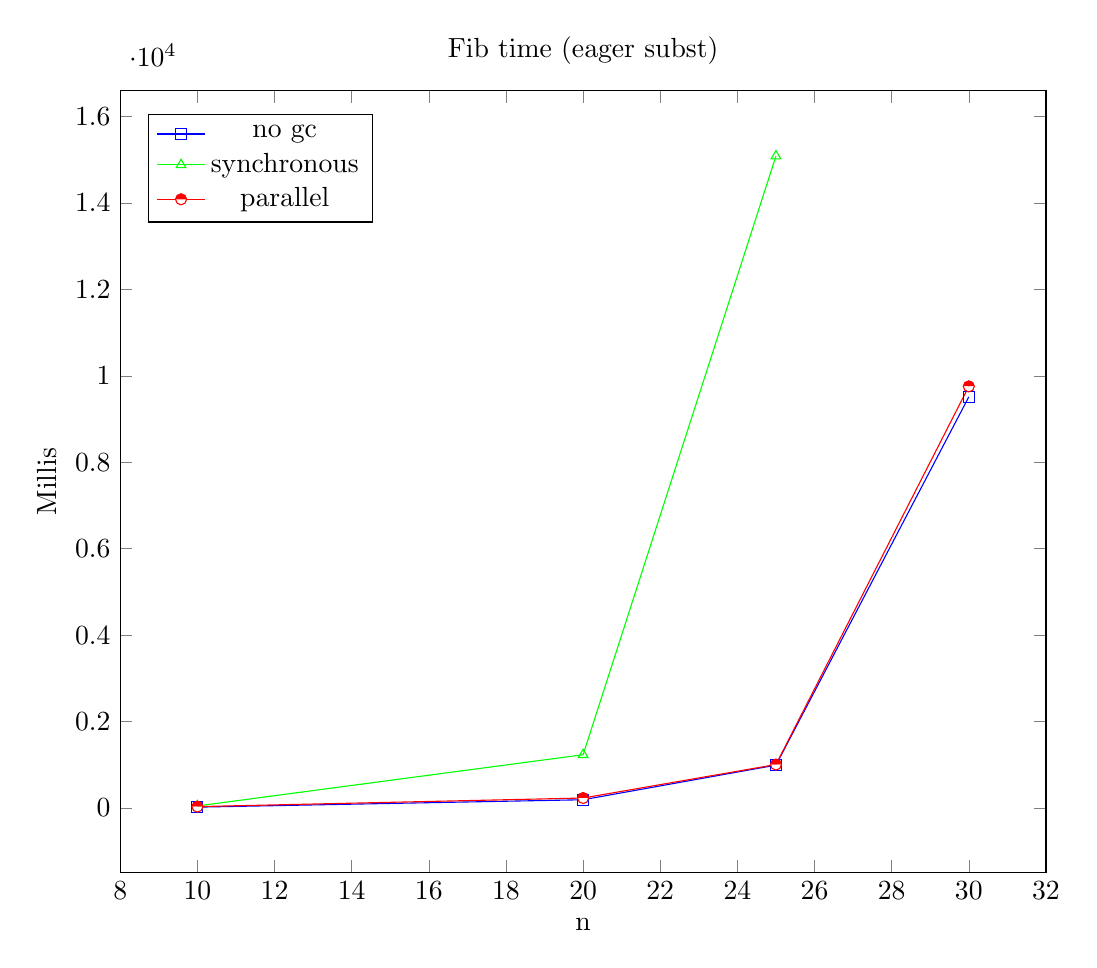
\begin{tikzpicture}
			\begin{axis}[
					title={Fib time (eager subst)},
					legend pos= north west,
					width=1.1\textwidth,
					xlabel={n},
					ylabel={Millis}
				]
				\addplot[
					color=blue,
					mark=square
				]
				coordinates {
						(10,19)  (20,190)  (25,991) (30,9512)
					};
				\addlegendentry{no gc}

				\addplot[
					color=green,
					mark=triangle
				]
				coordinates {
						(10,47)  (20,1232)  (25,15084)
					};
				\addlegendentry{synchronous}

				\addplot[
					color=red,
					mark=halfcircle*
				]
				coordinates {
						(10,31)  (20,230)  (25,1005) (30,9755)
					};
				\addlegendentry{parallel}
			\end{axis}
		\end{tikzpicture}
		%\caption{Fibonacci function time without trimming (no trimming)}
		%\label{fig:cps:benchmark1}
	\end{subfigure}
	\hfil
	\begin{subfigure}{0.49\textwidth}
		\centering
		\begin{tikzpicture}
			\begin{axis}[
					title={Fib final heap size (eager subst)},
					legend pos= north west,
					width=1.1\textwidth,
					xlabel={n},
					ylabel={Heap size}
				]
				\addplot[
					color=blue,
					mark=square
				]
				coordinates {
						(10,179)  (20,21893)  (25,242787) (30,2692539)
					};
				\addlegendentry{no gc}

				\addplot[
					color=green,
					mark=triangle
				]
				coordinates {
						(10,5)  (20,4)  (25,0)
					};
				\addlegendentry{synchronous}

				\addplot[
					color=red,
					mark=halfcircle*
				]
				coordinates {
						(10,39)  (20,130)  (25,11010) (30,770124)
					};
				\addlegendentry{parallel}
			\end{axis}
		\end{tikzpicture}
		%\caption{Fibonacci sequence heap size on program termination (no trimming)}
		%\label{fig:cps:benchmark2}
	\end{subfigure}
	\hspace*{-1cm}
	\begin{subfigure}{0.49\textwidth}
		\centering
		\begin{tikzpicture}
			\begin{axis}[
					title={Sum time (eager subst)},
					legend pos= north west,
					width={1.1\textwidth},
					xlabel={n},
					ylabel={Millis}
				]
				\addplot[
					color=blue,
					mark=square
				]
				coordinates {
						(100,22)  (1000,80)  (10000,473) (100000,3025)
					};
				\addlegendentry{no gc}

				\addplot[
					color=green,
					mark=triangle
				]
				coordinates {
						(100,138)  (1000,639)  (10000,4631) (100000,45240)
					};
				\addlegendentry{synchronous}

				\addplot[
					color=red,
					mark=halfcircle*
				]
				coordinates {
						(100,29)  (1000,89)  (10000,431) (100000,2949)
					};
				\addlegendentry{parallel}
			\end{axis}
		\end{tikzpicture}
		%\caption{Sum of integers $1 \dots n$ (no trimming)}
		%\label{fig:cps:benchmark2}
	\end{subfigure}
	\hfil
	\begin{subfigure}{0.49\textwidth}
		\centering
		\begin{tikzpicture}
			\begin{axis}[
					title={Fib time (environment)},
					legend pos= north west,
					width={1.1\textwidth},
					xlabel={n},
					ylabel={Millis}
				]
				\addplot[
					color=blue,
					mark=square
				]
				coordinates {
						(10,19)  (20,251)  (25,1166) (30,11659)
					};
				\addlegendentry{no gc}

				\addplot[
					color=green,
					mark=triangle
				]
				coordinates {
						(10,88)  (20,3242)  (25,46235)
					};
				\addlegendentry{synchronous}

				\addplot[
					color=red,
					mark=halfcircle*
				]
				coordinates {
						(10,31)  (20,287)  (25,1107) (30,12489)
					};
				\addlegendentry{parallel}
			\end{axis}
		\end{tikzpicture}
		%\caption{Sum of integers $1 \dots n$ (no trimming)}
		%\label{fig:cps:benchmark2}
	\end{subfigure}
	\hspace*{-1cm}
	\begin{subfigure}{0.49\textwidth}
		\centering
		\begin{tikzpicture}
			\begin{axis}[
					title={Sum time (environment)},
					legend pos= north west,
					width={1.1\textwidth},
					xlabel={n},
					ylabel={Millis}
				]
				\addplot[
					color=blue,
					mark=square
				]
				coordinates {
						(100,34)  (1000,114)  (10000,468) (100000,3615)
					};
				\addlegendentry{no gc}

				\addplot[
					color=green,
					mark=triangle
				]
				coordinates {
						(100,263)  (1000,1559)  (10000,13123)
					};
				\addlegendentry{synchronous}

				\addplot[
					color=red,
					mark=halfcircle*
				]
				coordinates {
						(100,36)  (1000,153)  (10000,571) (100000,2952)
					};
				\addlegendentry{parallel}
			\end{axis}
		\end{tikzpicture}
		%\caption{Sum of integers $1 \dots n$ (no trimming)}
		%\label{fig:cps:benchmark2}
	\end{subfigure}
	\hfil
	\begin{subfigure}{0.49\textwidth}
		\centering
		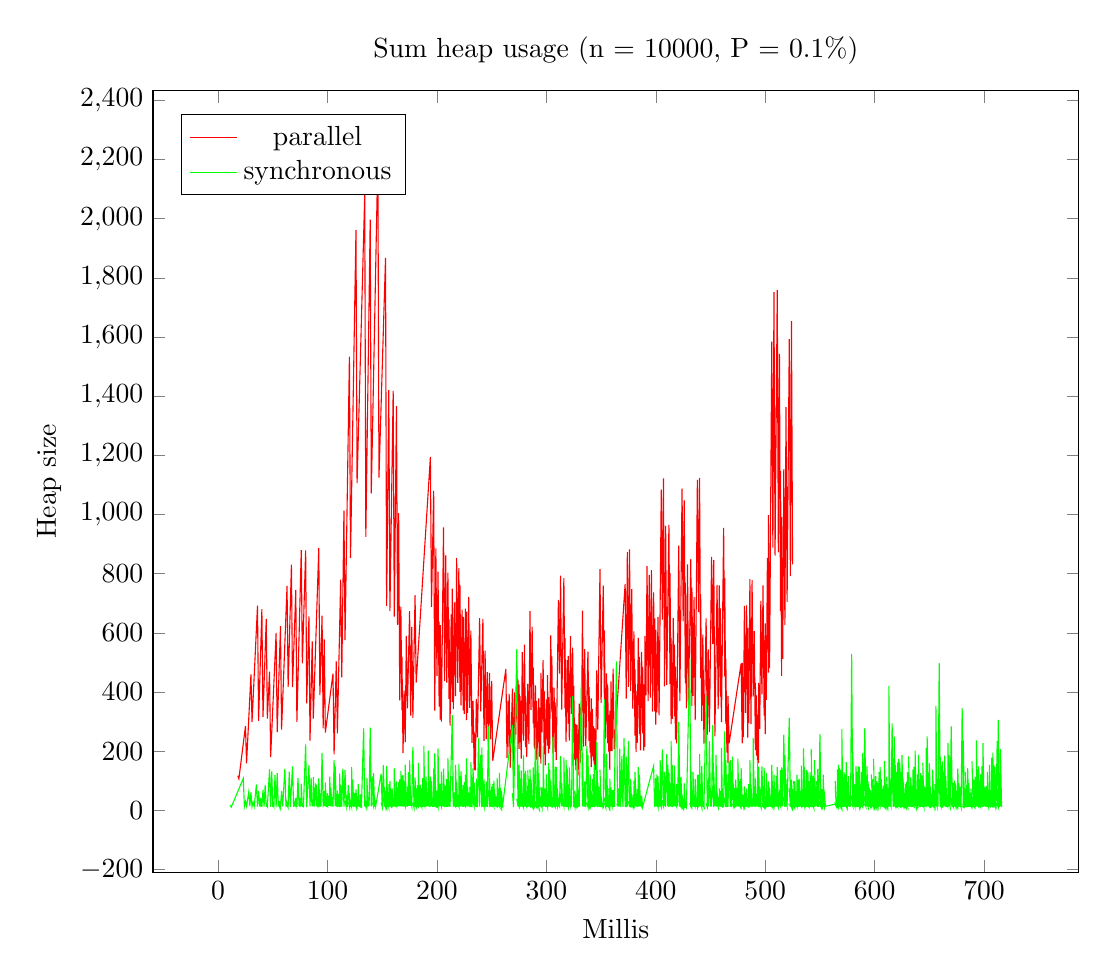
\begin{tikzpicture}
			\begin{axis}[
					title={Sum heap usage (n = 10000, P = 0.1\%)},
					legend pos= north west,
					width={1.1\textwidth},
					xlabel={Millis},
					ylabel={Heap size}
				]
				\addplot[
					color=red,
					%mark=square
				]
				coordinates {
						(18, 117) (19, 107)
						(25, 285) (26, 159)
						(30, 460) (31, 299)
						(36, 692) (37, 303)
						(40, 680) (41, 316)
						(44, 647) (45, 310)
						(47, 469) (48, 180)
						(53, 600) (54, 265)
						(57, 623) (58, 273)
						(63, 759) (64, 417)
						(67, 831) (68, 417)
						(71, 745) (72, 299)
						(76, 880) (77, 497)
						(80, 879) (81, 362)
						(83, 656) (84, 236)
						(86, 571) (87, 310)
						(92, 887) (93, 390)
						(95, 658) (96, 277)
						(97, 578) (98, 263)
						(105, 462) (106, 189)
						(108, 504) (109, 260)
						(112, 780) (113, 450)
						(115, 1013) (116, 576)
						(120, 1534) (121, 853)
						(126, 1962) (127, 1106)
						(134, 2082) (135, 925)
						(139, 1997) (140, 1072)
						(146, 2212) (147, 1125)
						(153, 1868) (154, 691)
						(156, 1421) (157, 674)
						(160, 1418) (161, 655)
						(163, 1367) (164, 627)
						(165, 1005) (166, 372)
						(167, 689) (168, 339)
						(168, 520) (169, 194)
						(170, 405) (171, 231)
						(172, 590) (173, 345)
						(175, 674) (176, 320)
						(177, 620) (178, 313)
						(180, 728) (181, 432)
						(194, 1195) (195, 688)
						(197, 1080) (198, 337)
						(199, 886) (200, 455)
						(201, 807) (202, 351)
						(202, 637) (203, 307)
						(203, 626) (204, 300)
						(206, 957) (207, 437)
						(208, 862) (209, 432)
						(210, 804) (211, 377)
						(211, 646) (212, 287)
						(213, 663) (214, 367)
						(214, 750) (215, 342)
						(216, 703) (217, 386)
						(218, 854) (219, 431)
						(220, 819) (221, 401)
						(221, 763) (222, 355)
						(223, 679) (224, 338)
						(224, 653) (225, 326)
						(226, 682) (227, 305)
						(227, 672) (228, 330)
						(229, 722) (230, 347)
						(231, 608) (232, 228)
						(233, 370) (234, 136)
						(234, 266) (235, 135)
						(236, 377) (237, 247)
						(239, 650) (240, 335)
						(242, 647) (243, 235)
						(244, 540) (245, 241)
						(246, 467) (247, 219)
						(248, 465) (249, 240)
						(250, 438) (251, 168)
						(263, 478) (264, 177)
						(265, 371) (266, 196)
						(266, 394) (267, 145)
						(269, 412) (270, 128)
						(271, 399) (272, 256)
						(273, 476) (274, 226)
						(274, 443) (275, 208)
						(275, 425) (276, 230)
						(276, 386) (277, 175)
						(278, 535) (279, 236)
						(280, 560) (281, 214)
						(281, 387) (282, 181)
						(283, 428) (284, 224)
						(285, 674) (286, 340)
						(287, 621) (288, 294)
						(288, 483) (289, 209)
						(290, 423) (291, 172)
						(291, 370) (292, 169)
						(293, 379) (294, 181)
						(294, 347) (295, 158)
						(295, 465) (296, 264)
						(297, 508) (298, 190)
						(298, 404) (299, 152)
						(300, 375) (301, 219)
						(301, 457) (302, 193)
						(302, 383) (303, 208)
						(304, 592) (305, 332)
						(305, 521) (306, 194)
						(307, 415) (308, 198)
						(308, 365) (309, 171)
						(311, 712) (312, 462)
						(313, 794) (314, 341)
						(316, 785) (317, 345)
						(317, 582) (318, 232)
						(319, 508) (320, 293)
						(320, 522) (321, 236)
						(322, 589) (323, 326)
						(324, 550) (325, 229)
						(325, 421) (326, 170)
						(326, 294) (327, 136)
						(327, 292) (328, 172)
						(328, 288) (329, 118)
						(330, 361) (331, 162)
						(331, 348) (332, 202)
						(333, 675) (334, 216)
						(335, 545) (336, 217)
						(338, 537) (339, 235)
						(339, 417) (340, 195)
						(340, 331) (341, 146)
						(341, 379) (342, 183)
						(342, 343) (343, 168)
						(343, 285) (344, 126)
						(344, 277) (345, 137)
						(346, 473) (347, 273)
						(349, 816) (350, 363)
						(352, 760) (353, 374)
						(353, 608) (354, 243)
						(355, 463) (356, 227)
						(356, 425) (357, 199)
						(357, 323) (358, 137)
						(358, 337) (359, 201)
						(359, 436) (360, 200)
						(361, 479) (362, 206)
						(372, 766) (373, 378)
						(374, 873) (375, 418)
						(376, 882) (377, 403)
						(378, 748) (379, 343)
						(380, 605) (381, 253)
						(381, 477) (382, 197)
						(382, 404) (383, 228)
						(384, 583) (385, 259)
						(385, 519) (386, 203)
						(387, 536) (388, 261)
						(388, 485) (389, 202)
						(389, 426) (390, 215)
						(390, 589) (391, 389)
						(392, 826) (393, 369)
						(394, 796) (395, 381)
						(396, 812) (397, 334)
						(398, 737) (399, 335)
						(399, 649) (400, 290)
						(400, 610) (401, 331)
						(402, 654) (403, 321)
						(405, 1084) (406, 645)
						(407, 1122) (408, 419)
						(409, 962) (410, 424)
						(412, 965) (413, 427)
						(413, 802) (414, 292)
						(414, 583) (415, 309)
						(416, 650) (417, 319)
						(417, 560) (418, 240)
						(418, 486) (419, 227)
						(421, 895) (422, 369)
						(424, 1088) (425, 639)
						(426, 1048) (427, 429)
						(427, 770) (428, 345)
						(429, 832) (430, 338)
						(432, 849) (433, 353)
						(433, 753) (434, 387)
						(435, 721) (436, 305)
						(438, 1117) (439, 670)
						(440, 1124) (441, 447)
						(441, 731) (442, 303)
						(443, 594) (444, 226)
						(446, 649) (447, 256)
						(448, 544) (449, 265)
						(451, 857) (452, 562)
						(453, 846) (454, 250)
						(456, 762) (457, 342)
						(458, 761) (459, 385)
						(459, 683) (460, 298)
						(462, 955) (463, 453)
						(463, 785) (464, 292)
						(464, 512) (465, 195)
						(465, 352) (466, 160)
						(466, 387) (467, 227)
						(478, 497) (479, 227)
						(479, 499) (480, 248)
						(481, 691) (482, 330)
						(483, 693) (484, 246)
						(484, 617) (485, 295)
						(486, 782) (487, 292)
						(488, 778) (489, 385)
						(490, 606) (491, 204)
						(491, 426) (492, 236)
						(491, 431) (492, 185)
						(492, 389) (493, 169)
						(493, 324) (494, 160)
						(494, 431) (495, 276)
						(496, 708) (497, 391)
						(498, 761) (499, 320)
						(499, 575) (500, 258)
						(500, 632) (501, 374)
						(502, 854) (503, 466)
						(503, 998) (504, 481)
						(506, 1585) (507, 888)
						(508, 1752) (509, 861)
						(511, 1759) (512, 872)
						(513, 1543) (514, 674)
						(514, 1148) (515, 455)
						(515, 991) (516, 512)
						(517, 1154) (518, 626)
						(519, 1363) (520, 705)
						(522, 1593) (523, 792)
						(524, 1654) (525, 832)
					};
				\addlegendentry{parallel}

				\addplot[
					color=green,
					%mark=triangle
				]
				coordinates {
						(11, 18) (12, 11)
						(23, 108) (24, 14)
						(25, 31) (26, 14)
						(28, 62) (29, 15)
						(30, 61) (31, 13)
						(32, 27) (33, 13)
						(35, 88) (36, 13)
						(37, 65) (38, 14)
						(38, 39) (39, 13)
						(39, 42) (40, 11)
						(41, 69) (42, 13)
						(43, 86) (44, 13)
						(44, 14) (45, 13)
						(44, 21) (45, 13)
						(47, 139) (48, 12)
						(49, 132) (50, 11)
						(50, 26) (51, 13)
						(52, 119) (53, 11)
						(54, 126) (55, 13)
						(55, 26) (56, 14)
						(56, 32) (57, 11)
						(58, 65) (59, 14)
						(61, 141) (62, 13)
						(62, 32) (63, 14)
						(62, 17) (63, 14)
						(63, 23) (64, 11)
						(65, 131) (66, 11)
						(68, 149) (69, 12)
						(69, 41) (70, 14)
						(70, 25) (71, 15)
						(71, 41) (72, 15)
						(71, 17) (72, 14)
						(73, 109) (74, 14)
						(74, 34) (75, 11)
						(75, 42) (76, 15)
						(76, 90) (77, 12)
						(77, 20) (78, 14)
						(80, 223) (81, 11)
						(83, 153) (84, 14)
						(85, 111) (86, 14)
						(85, 49) (86, 15)
						(86, 34) (87, 14)
						(87, 113) (88, 13)
						(89, 91) (90, 14)
						(90, 87) (91, 14)
						(90, 21) (91, 14)
						(91, 15) (92, 15)
						(92, 108) (93, 12)
						(93, 57) (94, 14)
						(95, 194) (96, 11)
						(96, 42) (97, 15)
						(97, 66) (98, 14)
						(98, 95) (99, 11)
						(99, 19) (100, 14)
						(99, 39) (100, 11)
						(100, 58) (101, 15)
						(101, 49) (102, 15)
						(102, 114) (103, 14)
						(103, 77) (104, 14)
						(104, 45) (105, 13)
						(106, 170) (107, 15)
						(107, 149) (108, 13)
						(108, 43) (109, 11)
						(108, 35) (109, 12)
						(109, 67) (110, 13)
						(110, 55) (111, 11)
						(111, 125) (112, 12)
						(112, 87) (113, 13)
						(114, 141) (115, 13)
						(116, 137) (117, 14)
						(116, 32) (117, 14)
						(117, 48) (118, 14)
						(117, 53) (118, 12)
						(119, 85) (120, 13)
						(119, 27) (120, 12)
						(120, 58) (121, 14)
						(120, 34) (121, 11)
						(121, 30) (122, 13)
						(122, 146) (123, 14)
						(123, 104) (124, 11)
						(124, 59) (125, 14)
						(125, 58) (126, 13)
						(125, 27) (126, 12)
						(126, 71) (127, 13)
						(126, 20) (127, 12)
						(127, 42) (128, 14)
						(127, 47) (128, 15)
						(128, 90) (129, 11)
						(129, 35) (130, 14)
						(129, 15) (130, 12)
						(130, 54) (131, 12)
						(130, 18) (131, 14)
						(133, 277) (134, 14)
						(134, 53) (135, 13)
						(134, 38) (135, 12)
						(134, 29) (135, 13)
						(135, 27) (136, 13)
						(136, 109) (137, 14)
						(137, 45) (138, 14)
						(139, 280) (140, 14)
						(141, 114) (142, 14)
						(141, 26) (142, 13)
						(142, 126) (143, 13)
						(143, 43) (144, 14)
						(143, 45) (144, 14)
						(149, 124) (150, 12)
						(149, 27) (150, 14)
						(151, 153) (152, 13)
						(151, 43) (152, 14)
						(152, 79) (153, 11)
						(152, 30) (153, 13)
						(153, 66) (154, 15)
						(153, 26) (154, 11)
						(154, 150) (155, 13)
						(155, 62) (156, 13)
						(155, 27) (156, 11)
						(156, 89) (157, 14)
						(157, 100) (158, 13)
						(157, 19) (158, 14)
						(158, 71) (159, 11)
						(158, 11) (159, 11)
						(159, 75) (160, 14)
						(159, 31) (160, 14)
						(159, 54) (160, 13)
						(160, 38) (161, 13)
						(160, 39) (161, 14)
						(161, 142) (162, 14)
						(161, 15) (162, 14)
						(162, 22) (163, 15)
						(162, 48) (163, 14)
						(163, 98) (164, 14)
						(164, 78) (165, 15)
						(164, 63) (165, 14)
						(165, 96) (166, 14)
						(166, 105) (167, 14)
						(167, 133) (168, 14)
						(168, 117) (169, 13)
						(168, 67) (169, 14)
						(169, 119) (170, 14)
						(170, 22) (171, 13)
						(170, 98) (171, 13)
						(171, 155) (172, 14)
						(172, 34) (173, 13)
						(172, 57) (173, 14)
						(173, 81) (174, 15)
						(174, 129) (175, 15)
						(175, 169) (176, 15)
						(176, 41) (177, 15)
						(176, 26) (177, 14)
						(176, 30) (177, 14)
						(178, 215) (179, 15)
						(178, 26) (179, 11)
						(179, 83) (180, 13)
						(180, 111) (181, 12)
						(180, 20) (181, 12)
						(180, 35) (181, 11)
						(180, 38) (181, 13)
						(180, 15) (181, 14)
						(181, 16) (182, 15)
						(181, 74) (182, 12)
						(182, 60) (183, 14)
						(182, 15) (183, 11)
						(182, 85) (183, 12)
						(183, 161) (184, 14)
						(184, 26) (185, 14)
						(184, 32) (185, 12)
						(185, 86) (186, 13)
						(185, 24) (186, 13)
						(185, 34) (186, 11)
						(186, 75) (187, 11)
						(186, 51) (187, 11)
						(187, 109) (188, 12)
						(188, 219) (189, 12)
						(188, 19) (189, 15)
						(189, 57) (190, 15)
						(189, 70) (190, 13)
						(190, 114) (191, 14)
						(191, 62) (192, 15)
						(192, 202) (193, 11)
						(192, 59) (193, 14)
						(193, 99) (194, 13)
						(194, 48) (195, 14)
						(194, 114) (195, 14)
						(195, 34) (196, 13)
						(195, 99) (196, 11)
						(196, 35) (197, 14)
						(197, 142) (198, 15)
						(198, 193) (199, 14)
						(198, 80) (199, 11)
						(199, 27) (200, 12)
						(199, 12) (200, 11)
						(199, 59) (200, 13)
						(200, 67) (201, 14)
						(200, 32) (201, 14)
						(201, 209) (202, 13)
						(202, 54) (203, 15)
						(203, 90) (204, 14)
						(203, 25) (204, 13)
						(204, 131) (205, 14)
						(204, 94) (205, 15)
						(205, 65) (206, 14)
						(205, 64) (206, 13)
						(206, 141) (207, 11)
						(206, 62) (207, 12)
						(207, 85) (208, 13)
						(207, 35) (208, 14)
						(208, 82) (209, 12)
						(209, 106) (210, 11)
						(209, 91) (210, 11)
						(210, 177) (211, 14)
						(211, 42) (212, 12)
						(211, 100) (212, 14)
						(214, 322) (215, 13)
						(214, 114) (215, 14)
						(215, 38) (216, 14)
						(215, 34) (216, 14)
						(215, 30) (216, 15)
						(215, 60) (216, 13)
						(216, 19) (217, 13)
						(216, 61) (217, 11)
						(217, 154) (218, 14)
						(217, 15) (218, 14)
						(218, 95) (219, 12)
						(218, 84) (219, 14)
						(219, 53) (220, 14)
						(219, 24) (220, 14)
						(220, 157) (221, 13)
						(220, 67) (221, 14)
						(221, 116) (222, 14)
						(222, 132) (223, 13)
						(222, 42) (223, 15)
						(223, 34) (224, 12)
						(223, 71) (224, 13)
						(223, 49) (224, 14)
						(224, 85) (225, 13)
						(225, 83) (226, 14)
						(225, 21) (226, 14)
						(225, 96) (226, 14)
						(226, 121) (227, 14)
						(227, 176) (228, 13)
						(228, 60) (229, 15)
						(228, 80) (229, 14)
						(229, 53) (230, 13)
						(229, 60) (230, 12)
						(229, 43) (230, 11)
						(230, 59) (231, 14)
						(230, 79) (231, 11)
						(231, 163) (232, 11)
						(233, 142) (234, 13)
						(233, 50) (234, 13)
						(233, 31) (234, 14)
						(234, 31) (235, 14)
						(234, 94) (235, 13)
						(235, 47) (236, 11)
						(236, 107) (237, 14)
						(236, 31) (237, 11)
						(236, 49) (237, 14)
						(238, 245) (239, 13)
						(240, 187) (241, 11)
						(241, 213) (242, 13)
						(242, 44) (243, 12)
						(242, 31) (243, 13)
						(243, 104) (244, 14)
						(243, 18) (244, 12)
						(243, 19) (244, 15)
						(243, 15) (244, 15)
						(244, 49) (245, 15)
						(245, 98) (246, 12)
						(247, 284) (248, 12)
						(247, 68) (248, 11)
						(248, 30) (249, 13)
						(248, 110) (249, 13)
						(249, 67) (250, 12)
						(250, 81) (251, 13)
						(250, 48) (251, 14)
						(250, 34) (251, 11)
						(251, 26) (252, 15)
						(251, 90) (252, 12)
						(252, 100) (253, 14)
						(253, 55) (254, 11)
						(253, 27) (254, 12)
						(253, 36) (254, 14)
						(254, 39) (255, 14)
						(254, 15) (255, 12)
						(254, 47) (255, 13)
						(255, 109) (256, 13)
						(256, 74) (257, 15)
						(256, 21) (257, 13)
						(256, 18) (257, 14)
						(257, 127) (258, 12)
						(258, 76) (259, 11)
						(258, 22) (259, 13)
						(258, 27) (259, 12)
						(259, 44) (260, 14)
						(259, 18) (260, 13)
						(259, 65) (260, 14)
						(269, 289) (270, 15)
						(269, 58) (270, 11)
						(273, 546) (274, 14)
						(273, 40) (274, 14)
						(274, 47) (275, 14)
						(274, 22) (275, 15)
						(274, 21) (275, 13)
						(275, 154) (276, 14)
						(275, 96) (276, 11)
						(276, 107) (277, 14)
						(277, 135) (278, 11)
						(277, 51) (278, 11)
						(278, 27) (279, 13)
						(278, 23) (279, 12)
						(278, 58) (279, 15)
						(279, 186) (280, 13)
						(280, 124) (281, 15)
						(281, 133) (282, 12)
						(281, 15) (282, 14)
						(281, 58) (282, 12)
						(281, 26) (282, 14)
						(282, 45) (283, 12)
						(282, 42) (283, 12)
						(283, 84) (284, 13)
						(283, 135) (284, 13)
						(284, 19) (285, 14)
						(284, 106) (285, 13)
						(285, 59) (286, 11)
						(285, 139) (286, 14)
						(286, 24) (287, 12)
						(286, 18) (287, 13)
						(286, 103) (287, 11)
						(287, 22) (288, 13)
						(288, 145) (289, 14)
						(288, 24) (289, 14)
						(288, 72) (289, 14)
						(288, 42) (289, 13)
						(290, 245) (291, 11)
						(290, 19) (291, 14)
						(290, 31) (291, 11)
						(291, 50) (292, 15)
						(292, 210) (293, 11)
						(292, 27) (293, 11)
						(292, 19) (293, 12)
						(292, 12) (293, 11)
						(293, 126) (294, 13)
						(293, 78) (294, 13)
						(294, 51) (295, 12)
						(294, 39) (295, 13)
						(294, 17) (295, 15)
						(294, 50) (295, 12)
						(295, 19) (296, 13)
						(295, 79) (296, 11)
						(295, 25) (296, 14)
						(295, 25) (296, 15)
						(296, 77) (297, 13)
						(297, 218) (298, 15)
						(298, 50) (299, 11)
						(298, 66) (299, 13)
						(298, 37) (299, 14)
						(299, 74) (300, 14)
						(299, 42) (300, 13)
						(299, 70) (300, 12)
						(300, 122) (301, 14)
						(300, 31) (301, 13)
						(301, 59) (302, 14)
						(301, 58) (302, 13)
						(302, 160) (303, 13)
						(302, 45) (303, 13)
						(303, 139) (304, 14)
						(304, 100) (305, 13)
						(304, 28) (305, 13)
						(304, 14) (305, 12)
						(304, 42) (305, 12)
						(305, 15) (306, 13)
						(306, 249) (307, 14)
						(307, 53) (308, 13)
						(307, 51) (308, 11)
						(307, 17) (308, 14)
						(307, 65) (308, 15)
						(308, 149) (309, 13)
						(309, 146) (310, 14)
						(309, 31) (310, 15)
						(310, 74) (311, 13)
						(310, 75) (311, 14)
						(311, 17) (312, 14)
						(311, 39) (312, 11)
						(311, 43) (312, 11)
						(311, 27) (312, 14)
						(311, 23) (312, 14)
						(313, 183) (314, 14)
						(313, 38) (314, 15)
						(313, 56) (314, 14)
						(314, 90) (315, 14)
						(314, 93) (315, 14)
						(315, 31) (316, 14)
						(316, 178) (317, 14)
						(316, 71) (317, 13)
						(317, 84) (318, 15)
						(317, 58) (318, 12)
						(317, 28) (318, 14)
						(317, 47) (318, 11)
						(318, 171) (319, 12)
						(319, 143) (320, 13)
						(319, 27) (320, 12)
						(320, 88) (321, 13)
						(321, 145) (322, 15)
						(321, 29) (322, 13)
						(321, 46) (322, 12)
						(322, 42) (323, 14)
						(322, 50) (323, 13)
						(322, 41) (323, 14)
						(324, 386) (325, 11)
						(325, 35) (326, 14)
						(325, 47) (326, 11)
						(325, 28) (326, 12)
						(326, 48) (327, 14)
						(326, 66) (327, 12)
						(326, 18) (327, 14)
						(327, 56) (328, 14)
						(327, 33) (328, 15)
						(327, 18) (328, 13)
						(328, 176) (329, 13)
						(328, 99) (329, 11)
						(329, 68) (330, 12)
						(329, 50) (330, 15)
						(332, 432) (333, 14)
						(333, 194) (334, 14)
						(333, 43) (334, 13)
						(334, 31) (335, 13)
						(334, 33) (335, 15)
						(334, 73) (335, 15)
						(335, 98) (336, 11)
						(335, 35) (336, 11)
						(337, 217) (338, 14)
						(337, 26) (338, 12)
						(338, 187) (339, 14)
						(338, 24) (339, 14)
						(338, 51) (339, 12)
						(339, 86) (340, 13)
						(339, 19) (340, 11)
						(340, 122) (341, 15)
						(340, 37) (341, 13)
						(340, 59) (341, 11)
						(341, 59) (342, 13)
						(341, 45) (342, 11)
						(341, 64) (342, 14)
						(342, 15) (343, 14)
						(342, 106) (343, 11)
						(343, 43) (344, 11)
						(343, 123) (344, 11)
						(344, 155) (345, 13)
						(345, 83) (346, 14)
						(346, 232) (347, 14)
						(346, 42) (347, 11)
						(347, 94) (348, 13)
						(347, 62) (348, 13)
						(348, 17) (349, 14)
						(348, 80) (349, 11)
						(349, 66) (350, 15)
						(349, 138) (350, 12)
						(350, 50) (351, 14)
						(350, 34) (351, 11)
						(350, 41) (351, 14)
						(350, 26) (351, 14)
						(351, 23) (352, 14)
						(353, 375) (354, 12)
						(353, 23) (354, 13)
						(353, 43) (354, 11)
						(354, 107) (355, 11)
						(354, 59) (355, 14)
						(355, 191) (356, 11)
						(355, 41) (356, 14)
						(356, 18) (357, 12)
						(356, 19) (357, 13)
						(356, 39) (357, 11)
						(356, 19) (357, 14)
						(356, 29) (357, 14)
						(357, 53) (358, 13)
						(357, 41) (358, 14)
						(357, 74) (358, 11)
						(357, 30) (358, 13)
						(358, 107) (359, 14)
						(358, 55) (359, 14)
						(359, 78) (360, 15)
						(359, 33) (360, 13)
						(359, 25) (360, 13)
						(360, 59) (361, 13)
						(360, 61) (361, 11)
						(360, 68) (361, 12)
						(361, 69) (362, 12)
						(361, 50) (362, 13)
						(361, 45) (362, 14)
						(364, 504) (365, 14)
						(365, 49) (366, 15)
						(365, 15) (366, 15)
						(365, 69) (366, 13)
						(366, 74) (367, 15)
						(367, 209) (368, 15)
						(367, 16) (368, 14)
						(369, 184) (370, 12)
						(369, 92) (370, 12)
						(371, 244) (372, 11)
						(372, 99) (373, 11)
						(373, 182) (374, 13)
						(375, 235) (376, 14)
						(375, 31) (376, 11)
						(376, 54) (377, 13)
						(376, 18) (377, 14)
						(377, 106) (378, 13)
						(377, 43) (378, 11)
						(377, 61) (378, 12)
						(378, 43) (379, 14)
						(378, 26) (379, 13)
						(378, 34) (379, 15)
						(378, 26) (379, 13)
						(379, 53) (380, 11)
						(379, 33) (380, 14)
						(379, 18) (380, 11)
						(380, 82) (381, 15)
						(380, 101) (381, 13)
						(381, 130) (382, 15)
						(382, 25) (383, 15)
						(382, 26) (383, 11)
						(382, 38) (383, 13)
						(383, 72) (384, 13)
						(384, 146) (385, 14)
						(384, 62) (385, 15)
						(385, 65) (386, 15)
						(385, 120) (386, 14)
						(386, 38) (387, 13)
						(386, 21) (387, 13)
						(386, 50) (387, 15)
						(387, 50) (388, 12)
						(398, 150) (399, 12)
						(399, 50) (400, 15)
						(399, 56) (400, 14)
						(400, 109) (401, 13)
						(401, 122) (402, 15)
						(401, 29) (402, 13)
						(402, 115) (403, 11)
						(403, 66) (404, 15)
						(404, 170) (405, 12)
						(404, 20) (405, 11)
						(404, 61) (405, 12)
						(406, 206) (407, 13)
						(406, 35) (407, 12)
						(406, 23) (407, 13)
						(407, 74) (408, 15)
						(408, 130) (409, 14)
						(408, 79) (409, 11)
						(410, 190) (411, 13)
						(411, 155) (412, 11)
						(411, 34) (412, 14)
						(412, 128) (413, 14)
						(413, 92) (414, 13)
						(414, 234) (415, 11)
						(415, 153) (416, 14)
						(416, 90) (417, 14)
						(417, 151) (418, 14)
						(418, 42) (419, 12)
						(418, 26) (419, 12)
						(418, 26) (419, 14)
						(419, 89) (420, 15)
						(421, 299) (422, 12)
						(421, 91) (422, 14)
						(422, 53) (423, 14)
						(422, 21) (423, 13)
						(422, 59) (423, 11)
						(423, 112) (424, 14)
						(423, 26) (424, 11)
						(423, 19) (424, 14)
						(424, 54) (425, 15)
						(424, 49) (425, 15)
						(424, 26) (425, 11)
						(425, 30) (426, 13)
						(425, 17) (426, 13)
						(425, 15) (426, 11)
						(426, 91) (427, 14)
						(426, 70) (427, 15)
						(426, 34) (427, 14)
						(427, 23) (428, 12)
						(431, 514) (432, 14)
						(431, 25) (432, 14)
						(432, 147) (433, 13)
						(432, 30) (433, 13)
						(432, 29) (433, 13)
						(432, 22) (433, 12)
						(433, 56) (434, 14)
						(434, 130) (435, 11)
						(434, 70) (435, 13)
						(435, 54) (436, 13)
						(435, 44) (436, 12)
						(435, 25) (436, 14)
						(436, 106) (437, 14)
						(436, 41) (437, 12)
						(437, 43) (438, 11)
						(437, 27) (438, 12)
						(438, 120) (439, 13)
						(438, 16) (439, 14)
						(438, 40) (439, 14)
						(439, 121) (440, 14)
						(440, 190) (441, 14)
						(441, 24) (442, 14)
						(441, 68) (442, 13)
						(441, 27) (442, 11)
						(442, 150) (443, 13)
						(443, 15) (444, 14)
						(443, 29) (444, 13)
						(443, 19) (444, 11)
						(446, 387) (447, 12)
						(446, 23) (447, 13)
						(446, 24) (447, 14)
						(447, 101) (448, 13)
						(449, 234) (450, 15)
						(449, 85) (450, 13)
						(450, 58) (451, 13)
						(452, 288) (453, 12)
						(452, 83) (453, 15)
						(453, 129) (454, 15)
						(454, 64) (455, 14)
						(455, 188) (456, 13)
						(455, 43) (456, 14)
						(456, 46) (457, 13)
						(456, 63) (457, 11)
						(456, 22) (457, 13)
						(457, 43) (458, 14)
						(457, 38) (458, 15)
						(457, 45) (458, 13)
						(458, 54) (459, 13)
						(458, 74) (459, 15)
						(459, 66) (460, 11)
						(460, 211) (461, 12)
						(460, 15) (461, 13)
						(461, 59) (462, 11)
						(463, 267) (464, 11)
						(463, 30) (464, 13)
						(463, 42) (464, 15)
						(464, 170) (465, 11)
						(465, 35) (466, 12)
						(465, 122) (466, 14)
						(467, 165) (468, 13)
						(468, 170) (469, 15)
						(468, 42) (469, 11)
						(470, 182) (471, 13)
						(470, 22) (471, 13)
						(470, 75) (471, 11)
						(471, 19) (472, 12)
						(471, 88) (472, 13)
						(472, 41) (473, 14)
						(472, 50) (473, 12)
						(472, 75) (473, 15)
						(473, 104) (474, 14)
						(474, 61) (475, 13)
						(474, 75) (475, 14)
						(475, 175) (476, 13)
						(476, 99) (477, 14)
						(476, 21) (477, 13)
						(477, 22) (478, 13)
						(477, 106) (478, 14)
						(478, 144) (479, 14)
						(479, 18) (480, 13)
						(479, 26) (480, 15)
						(479, 54) (480, 13)
						(479, 17) (480, 14)
						(479, 29) (480, 14)
						(480, 53) (481, 13)
						(480, 19) (481, 12)
						(480, 43) (481, 15)
						(481, 81) (482, 15)
						(481, 45) (482, 13)
						(482, 34) (483, 15)
						(482, 26) (483, 12)
						(482, 59) (483, 14)
						(482, 51) (483, 12)
						(483, 66) (484, 14)
						(483, 74) (484, 13)
						(484, 26) (485, 15)
						(484, 34) (485, 11)
						(484, 11) (485, 11)
						(485, 89) (486, 14)
						(485, 34) (486, 12)
						(486, 170) (487, 14)
						(487, 87) (488, 14)
						(487, 50) (488, 11)
						(488, 41) (489, 14)
						(489, 245) (490, 13)
						(490, 74) (491, 13)
						(491, 108) (492, 13)
						(491, 47) (492, 13)
						(492, 56) (493, 14)
						(493, 170) (494, 11)
						(494, 147) (495, 14)
						(494, 47) (495, 11)
						(495, 78) (496, 13)
						(495, 18) (496, 14)
						(495, 26) (496, 13)
						(495, 75) (496, 13)
						(497, 149) (498, 11)
						(497, 101) (498, 13)
						(497, 17) (498, 14)
						(498, 23) (499, 14)
						(498, 82) (499, 11)
						(498, 18) (499, 14)
						(499, 144) (500, 13)
						(499, 24) (500, 13)
						(500, 18) (501, 14)
						(500, 47) (501, 13)
						(500, 45) (501, 12)
						(500, 36) (501, 14)
						(501, 127) (502, 12)
						(502, 67) (503, 14)
						(502, 59) (503, 12)
						(503, 98) (504, 14)
						(504, 70) (505, 14)
						(504, 33) (505, 15)
						(504, 77) (505, 12)
						(505, 49) (506, 15)
						(505, 29) (506, 12)
						(505, 21) (506, 13)
						(505, 18) (506, 14)
						(506, 154) (507, 12)
						(506, 18) (507, 11)
						(507, 83) (508, 11)
						(507, 30) (508, 13)
						(507, 22) (508, 13)
						(508, 119) (509, 13)
						(509, 74) (510, 14)
						(510, 117) (511, 14)
						(511, 146) (512, 11)
						(511, 14) (512, 13)
						(511, 67) (512, 14)
						(511, 25) (512, 12)
						(512, 27) (513, 14)
						(512, 55) (513, 14)
						(513, 69) (514, 14)
						(513, 25) (514, 15)
						(514, 136) (515, 14)
						(515, 145) (516, 14)
						(517, 256) (518, 11)
						(517, 46) (518, 13)
						(518, 187) (519, 14)
						(519, 28) (520, 14)
						(519, 105) (520, 15)
						(522, 313) (523, 15)
						(522, 74) (523, 12)
						(523, 21) (524, 11)
						(523, 53) (524, 12)
						(523, 16) (524, 14)
						(523, 26) (524, 14)
						(524, 104) (525, 12)
						(524, 46) (525, 13)
						(524, 27) (525, 11)
						(525, 23) (526, 13)
						(525, 72) (526, 14)
						(526, 65) (527, 13)
						(526, 23) (527, 15)
						(526, 100) (527, 12)
						(527, 98) (528, 15)
						(527, 42) (528, 11)
						(528, 18) (529, 15)
						(528, 65) (529, 15)
						(528, 25) (529, 15)
						(529, 120) (530, 14)
						(530, 65) (531, 14)
						(530, 14) (531, 13)
						(530, 103) (531, 12)
						(531, 107) (532, 14)
						(532, 31) (533, 13)
						(532, 32) (533, 14)
						(532, 18) (533, 13)
						(532, 66) (533, 13)
						(533, 151) (534, 11)
						(534, 38) (535, 13)
						(535, 210) (536, 15)
						(535, 26) (536, 11)
						(535, 30) (536, 13)
						(536, 147) (537, 12)
						(536, 12) (537, 12)
						(537, 76) (538, 14)
						(537, 38) (538, 15)
						(537, 45) (538, 13)
						(538, 136) (539, 13)
						(538, 15) (539, 15)
						(539, 130) (540, 12)
						(539, 105) (540, 13)
						(539, 21) (540, 13)
						(540, 99) (541, 11)
						(540, 75) (541, 13)
						(540, 44) (541, 13)
						(541, 72) (542, 11)
						(541, 130) (542, 14)
						(541, 40) (542, 11)
						(542, 42) (543, 14)
						(542, 208) (543, 11)
						(543, 44) (544, 12)
						(543, 27) (544, 11)
						(543, 19) (544, 11)
						(543, 115) (544, 11)
						(543, 19) (544, 13)
						(544, 81) (545, 13)
						(544, 36) (545, 12)
						(544, 118) (545, 13)
						(545, 66) (546, 15)
						(545, 170) (546, 14)
						(546, 70) (547, 15)
						(546, 49) (547, 15)
						(546, 81) (547, 14)
						(547, 41) (548, 12)
						(547, 99) (548, 12)
						(548, 140) (549, 14)
						(548, 59) (549, 13)
						(548, 139) (549, 12)
						(550, 258) (551, 15)
						(550, 25) (551, 14)
						(550, 64) (551, 12)
						(550, 20) (551, 13)
						(550, 31) (551, 12)
						(551, 30) (552, 13)
						(551, 27) (552, 14)
						(551, 50) (552, 13)
						(551, 42) (552, 15)
						(551, 22) (552, 13)
						(552, 72) (553, 14)
						(552, 42) (553, 12)
						(552, 58) (553, 14)
						(553, 106) (554, 14)
						(553, 121) (554, 12)
						(553, 27) (554, 11)
						(553, 51) (554, 12)
						(554, 64) (555, 13)
						(554, 32) (555, 14)
						(564, 21) (565, 13)
						(564, 99) (565, 11)
						(564, 77) (565, 12)
						(565, 41) (566, 14)
						(565, 18) (566, 11)
						(565, 34) (566, 13)
						(566, 139) (567, 13)
						(566, 51) (567, 14)
						(566, 55) (567, 14)
						(566, 54) (567, 15)
						(566, 21) (567, 12)
						(567, 69) (568, 13)
						(567, 155) (568, 12)
						(568, 143) (569, 12)
						(568, 25) (569, 15)
						(569, 137) (570, 15)
						(569, 26) (570, 12)
						(569, 79) (570, 13)
						(570, 275) (571, 12)
						(570, 32) (571, 13)
						(571, 112) (572, 14)
						(571, 82) (572, 13)
						(571, 31) (572, 12)
						(572, 48) (573, 13)
						(572, 129) (573, 15)
						(573, 122) (574, 12)
						(573, 31) (574, 13)
						(573, 26) (574, 15)
						(573, 64) (574, 14)
						(574, 163) (575, 12)
						(574, 98) (575, 13)
						(574, 31) (575, 14)
						(575, 85) (576, 14)
						(575, 96) (576, 14)
						(576, 64) (577, 14)
						(576, 50) (577, 12)
						(576, 116) (577, 14)
						(577, 50) (578, 13)
						(579, 529) (580, 14)
						(579, 50) (580, 14)
						(579, 23) (580, 14)
						(580, 199) (581, 13)
						(580, 49) (581, 13)
						(581, 90) (582, 14)
						(581, 63) (582, 11)
						(581, 32) (582, 14)
						(582, 88) (583, 14)
						(582, 41) (583, 15)
						(582, 42) (583, 11)
						(582, 33) (583, 14)
						(583, 149) (584, 13)
						(583, 74) (584, 15)
						(583, 83) (584, 12)
						(584, 131) (585, 14)
						(584, 111) (585, 12)
						(585, 42) (586, 14)
						(585, 149) (586, 12)
						(585, 29) (586, 13)
						(586, 147) (587, 12)
						(586, 28) (587, 14)
						(587, 87) (588, 11)
						(587, 49) (588, 14)
						(587, 81) (588, 15)
						(588, 130) (589, 13)
						(588, 44) (589, 15)
						(588, 18) (589, 11)
						(589, 194) (590, 15)
						(591, 277) (592, 13)
						(591, 22) (592, 13)
						(591, 115) (592, 12)
						(591, 47) (592, 13)
						(592, 72) (593, 14)
						(592, 73) (593, 15)
						(593, 149) (594, 12)
						(593, 24) (594, 14)
						(593, 69) (594, 13)
						(593, 58) (594, 15)
						(594, 64) (595, 14)
						(594, 66) (595, 12)
						(594, 98) (595, 14)
						(595, 62) (596, 13)
						(595, 21) (596, 13)
						(595, 78) (596, 13)
						(595, 30) (596, 13)
						(595, 22) (596, 13)
						(596, 46) (597, 13)
						(596, 59) (597, 14)
						(596, 69) (597, 14)
						(596, 21) (597, 13)
						(596, 49) (597, 14)
						(597, 50) (598, 14)
						(597, 122) (598, 13)
						(598, 105) (599, 14)
						(598, 30) (599, 13)
						(598, 34) (599, 11)
						(598, 18) (599, 15)
						(598, 26) (599, 12)
						(599, 84) (600, 11)
						(599, 174) (600, 13)
						(599, 26) (600, 15)
						(600, 26) (601, 14)
						(600, 87) (601, 11)
						(600, 83) (601, 11)
						(600, 19) (601, 12)
						(601, 116) (602, 12)
						(601, 25) (602, 13)
						(601, 93) (602, 13)
						(602, 25) (603, 14)
						(602, 25) (603, 13)
						(602, 23) (603, 13)
						(602, 47) (603, 13)
						(602, 99) (603, 11)
						(603, 74) (604, 13)
						(603, 92) (604, 13)
						(604, 109) (605, 12)
						(604, 129) (605, 15)
						(604, 26) (605, 12)
						(604, 55) (605, 13)
						(605, 74) (606, 15)
						(605, 146) (606, 14)
						(606, 60) (607, 13)
						(606, 106) (607, 11)
						(607, 73) (608, 14)
						(607, 70) (608, 13)
						(607, 57) (608, 14)
						(607, 19) (608, 13)
						(607, 16) (608, 14)
						(608, 59) (609, 12)
						(608, 83) (609, 14)
						(609, 167) (610, 11)
						(609, 23) (610, 13)
						(609, 25) (610, 13)
						(609, 79) (610, 15)
						(609, 40) (610, 14)
						(610, 34) (611, 11)
						(610, 22) (611, 13)
						(610, 41) (611, 14)
						(610, 89) (611, 15)
						(611, 82) (612, 12)
						(611, 23) (612, 13)
						(611, 113) (612, 14)
						(612, 77) (613, 13)
						(613, 421) (614, 13)
						(614, 77) (615, 12)
						(614, 49) (615, 14)
						(614, 26) (615, 14)
						(614, 103) (615, 14)
						(616, 294) (617, 13)
						(616, 130) (617, 12)
						(617, 176) (618, 14)
						(618, 249) (619, 15)
						(618, 55) (619, 13)
						(618, 21) (619, 13)
						(619, 62) (620, 13)
						(619, 17) (620, 15)
						(619, 154) (620, 11)
						(620, 129) (621, 14)
						(620, 20) (621, 13)
						(620, 70) (621, 13)
						(620, 41) (621, 14)
						(621, 162) (622, 11)
						(622, 174) (623, 13)
						(622, 34) (623, 13)
						(622, 39) (623, 14)
						(622, 14) (623, 14)
						(622, 22) (623, 15)
						(623, 162) (624, 14)
						(623, 15) (624, 11)
						(624, 129) (625, 14)
						(624, 42) (625, 12)
						(625, 187) (626, 15)
						(625, 26) (626, 11)
						(625, 67) (626, 14)
						(625, 50) (626, 12)
						(626, 106) (627, 11)
						(626, 43) (627, 11)
						(626, 34) (627, 15)
						(626, 25) (627, 15)
						(626, 89) (627, 15)
						(627, 44) (628, 12)
						(627, 18) (628, 14)
						(627, 22) (628, 14)
						(627, 48) (628, 11)
						(627, 16) (628, 13)
						(627, 58) (628, 11)
						(628, 75) (629, 11)
						(628, 17) (629, 14)
						(628, 89) (629, 14)
						(628, 31) (629, 15)
						(629, 96) (630, 14)
						(629, 80) (630, 14)
						(629, 24) (630, 14)
						(629, 41) (630, 14)
						(630, 118) (631, 14)
						(630, 129) (631, 15)
						(631, 43) (632, 12)
						(631, 183) (632, 13)
						(631, 15) (632, 14)
						(632, 34) (633, 14)
						(632, 26) (633, 13)
						(632, 42) (633, 15)
						(632, 74) (633, 13)
						(633, 112) (634, 13)
						(633, 43) (634, 11)
						(633, 59) (634, 11)
						(633, 27) (634, 13)
						(633, 34) (634, 13)
						(634, 82) (635, 11)
						(634, 83) (635, 11)
						(634, 70) (635, 12)
						(635, 138) (636, 11)
						(635, 27) (636, 12)
						(635, 16) (636, 13)
						(635, 67) (636, 12)
						(636, 147) (637, 15)
						(637, 202) (638, 11)
						(637, 26) (638, 14)
						(637, 35) (638, 13)
						(637, 84) (638, 12)
						(638, 26) (639, 15)
						(638, 17) (639, 14)
						(638, 22) (639, 15)
						(638, 17) (639, 14)
						(638, 47) (639, 12)
						(638, 71) (639, 13)
						(638, 19) (639, 11)
						(639, 122) (640, 15)
						(640, 154) (641, 12)
						(640, 188) (641, 12)
						(640, 36) (641, 11)
						(641, 105) (642, 14)
						(641, 42) (642, 11)
						(641, 59) (642, 13)
						(642, 126) (643, 12)
						(642, 94) (643, 13)
						(642, 41) (643, 14)
						(643, 34) (644, 11)
						(643, 118) (644, 13)
						(643, 15) (644, 13)
						(643, 72) (644, 14)
						(644, 41) (645, 15)
						(644, 29) (645, 13)
						(644, 161) (645, 14)
						(645, 85) (646, 13)
						(645, 78) (646, 13)
						(646, 78) (647, 13)
						(646, 43) (647, 11)
						(646, 44) (647, 12)
						(647, 211) (648, 14)
						(647, 46) (648, 15)
						(647, 66) (648, 14)
						(648, 250) (649, 13)
						(649, 19) (650, 13)
						(649, 128) (650, 13)
						(650, 114) (651, 13)
						(650, 159) (651, 14)
						(650, 15) (651, 11)
						(651, 80) (652, 13)
						(651, 17) (652, 14)
						(651, 79) (652, 12)
						(651, 71) (652, 13)
						(652, 31) (653, 13)
						(652, 48) (653, 14)
						(652, 56) (653, 14)
						(652, 49) (653, 15)
						(653, 138) (654, 14)
						(653, 63) (654, 11)
						(653, 27) (654, 14)
						(653, 66) (654, 13)
						(654, 67) (655, 11)
						(654, 42) (655, 14)
						(654, 24) (655, 14)
						(654, 37) (655, 14)
						(655, 89) (656, 15)
						(656, 353) (657, 15)
						(656, 31) (657, 14)
						(657, 69) (658, 13)
						(657, 42) (658, 15)
						(659, 498) (660, 11)
						(659, 107) (660, 14)
						(660, 181) (661, 14)
						(660, 17) (661, 14)
						(660, 23) (661, 12)
						(661, 151) (662, 13)
						(661, 16) (662, 14)
						(661, 37) (662, 13)
						(661, 35) (662, 11)
						(662, 166) (663, 13)
						(662, 78) (663, 13)
						(663, 130) (664, 15)
						(664, 185) (665, 15)
						(664, 17) (665, 14)
						(664, 99) (665, 13)
						(665, 35) (666, 12)
						(665, 96) (666, 14)
						(665, 117) (666, 13)
						(666, 19) (667, 12)
						(667, 227) (668, 15)
						(667, 149) (668, 13)
						(668, 187) (669, 13)
						(668, 27) (669, 14)
						(668, 90) (669, 13)
						(670, 284) (671, 15)
						(670, 42) (671, 12)
						(670, 36) (671, 11)
						(670, 25) (671, 14)
						(670, 34) (671, 12)
						(671, 84) (672, 15)
						(671, 17) (672, 14)
						(671, 66) (672, 13)
						(671, 19) (672, 11)
						(671, 43) (672, 14)
						(672, 53) (673, 14)
						(672, 93) (673, 13)
						(673, 98) (674, 15)
						(673, 25) (674, 14)
						(673, 84) (674, 13)
						(673, 101) (674, 13)
						(674, 91) (675, 12)
						(674, 60) (675, 14)
						(674, 23) (675, 11)
						(674, 18) (675, 15)
						(674, 26) (675, 14)
						(675, 50) (676, 13)
						(675, 67) (676, 14)
						(675, 63) (676, 11)
						(675, 17) (676, 14)
						(676, 141) (677, 13)
						(676, 46) (677, 13)
						(676, 33) (677, 14)
						(677, 91) (678, 12)
						(677, 46) (678, 13)
						(677, 32) (678, 13)
						(677, 28) (678, 13)
						(677, 51) (678, 12)
						(678, 60) (679, 14)
						(678, 66) (679, 13)
						(678, 13) (679, 13)
						(678, 26) (679, 14)
						(678, 24) (679, 11)
						(678, 79) (679, 13)
						(680, 346) (681, 11)
						(680, 14) (681, 12)
						(681, 237) (682, 13)
						(681, 75) (682, 14)
						(681, 18) (682, 12)
						(682, 57) (683, 15)
						(682, 60) (683, 12)
						(682, 27) (683, 12)
						(682, 75) (683, 15)
						(683, 64) (684, 14)
						(683, 129) (684, 13)
						(683, 15) (684, 14)
						(684, 63) (685, 11)
						(684, 62) (685, 13)
						(684, 86) (685, 13)
						(685, 143) (686, 13)
						(685, 66) (686, 11)
						(685, 50) (686, 15)
						(686, 93) (687, 13)
						(686, 67) (687, 13)
						(686, 36) (687, 15)
						(686, 26) (687, 14)
						(686, 39) (687, 12)
						(687, 21) (688, 14)
						(687, 55) (688, 12)
						(687, 60) (688, 14)
						(687, 39) (688, 14)
						(687, 34) (688, 13)
						(688, 46) (689, 13)
						(688, 35) (689, 11)
						(688, 34) (689, 13)
						(688, 42) (689, 13)
						(688, 74) (689, 15)
						(688, 25) (689, 15)
						(689, 17) (690, 14)
						(689, 166) (690, 15)
						(690, 77) (691, 13)
						(690, 59) (691, 14)
						(690, 106) (691, 12)
						(690, 18) (691, 11)
						(690, 14) (691, 13)
						(691, 57) (692, 14)
						(691, 33) (692, 15)
						(691, 102) (692, 13)
						(691, 42) (692, 11)
						(692, 113) (693, 14)
						(693, 237) (694, 13)
						(694, 139) (695, 13)
						(694, 43) (695, 14)
						(694, 101) (695, 12)
						(694, 16) (695, 15)
						(694, 25) (695, 15)
						(695, 149) (696, 13)
						(695, 59) (696, 11)
						(696, 98) (697, 15)
						(696, 21) (697, 13)
						(696, 86) (697, 13)
						(696, 19) (697, 11)
						(697, 122) (698, 15)
						(697, 32) (698, 14)
						(697, 33) (698, 15)
						(697, 77) (698, 13)
						(698, 150) (699, 13)
						(698, 75) (699, 11)
						(699, 227) (700, 14)
						(700, 39) (701, 14)
						(700, 30) (701, 13)
						(700, 74) (701, 13)
						(700, 34) (701, 15)
						(700, 61) (701, 13)
						(701, 78) (702, 12)
						(701, 58) (702, 14)
						(701, 42) (702, 13)
						(701, 30) (702, 13)
						(701, 35) (702, 14)
						(702, 54) (703, 15)
						(702, 82) (703, 13)
						(702, 45) (703, 14)
						(702, 55) (703, 12)
						(703, 130) (704, 14)
						(703, 21) (704, 13)
						(703, 35) (704, 14)
						(703, 30) (704, 14)
						(704, 38) (705, 14)
						(704, 58) (705, 11)
						(704, 70) (705, 12)
						(705, 154) (706, 14)
						(705, 15) (706, 12)
						(705, 111) (706, 13)
						(706, 43) (707, 14)
						(706, 45) (707, 14)
						(707, 178) (708, 12)
						(707, 15) (708, 13)
						(707, 167) (708, 13)
						(708, 90) (709, 11)
						(708, 195) (709, 12)
						(709, 154) (710, 14)
						(709, 28) (710, 12)
						(709, 22) (710, 13)
						(710, 42) (711, 15)
						(710, 57) (711, 15)
						(710, 18) (711, 11)
						(710, 147) (711, 14)
						(712, 234) (713, 13)
						(712, 17) (713, 15)
						(712, 25) (713, 13)
						(712, 71) (713, 13)
						(712, 21) (713, 12)
						(712, 44) (713, 15)
						(713, 306) (714, 12)
						(714, 76) (715, 14)
						(715, 207) (716, 12)
						(715, 68) (716, 14)
					};
				\addlegendentry{synchronous}

				%\addplot[
				%color=blue,
				%mark=halfcircle*
				%]
				%coordinates {
				%(10,31)  (20,287)  (25,1107) (30,12489)
				%};
				%\addlegendentry{no gc}
			\end{axis}
		\end{tikzpicture}
		%\caption{Sum of integers $1 \dots n$ (no trimming)}
		%\label{fig:cps:benchmark2}
	\end{subfigure}
	%\hspace*{1cm}
	\begin{subfigure}{1\textwidth}
		\centering
		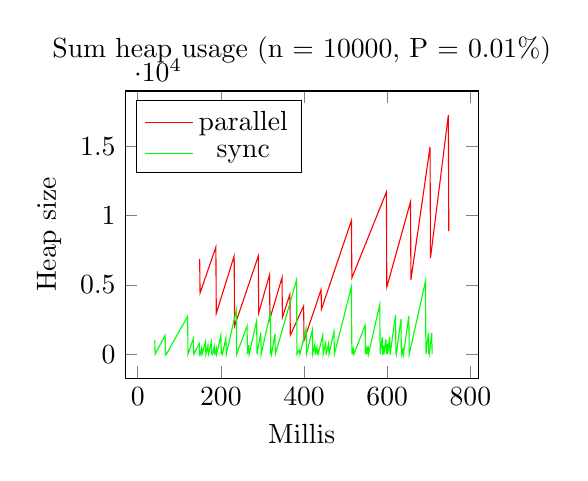
\begin{tikzpicture}
			\begin{axis}[
					title={Sum heap usage (n = 10000, P = 0.01\%)},
					legend pos= north west,
					width={0.5\textwidth},
					xlabel={Millis},
					ylabel={Heap size}
				]
				\addplot[
					color=red,
					%mark=square
				]
				coordinates {
						(149, 6890) (150, 4422)
						(188, 7739) (189, 2957)
						(232, 7097) (233, 2038)
						(290, 7086) (291, 2995)
						(317, 5737) (318, 2571)
						(347, 5531) (348, 2670)
						(366, 4337) (367, 1378)
						(399, 3488) (400, 1018)
						(441, 4663) (442, 3268)
						(514, 9658) (515, 5514)
						(598, 11705) (599, 4847)
						(656, 11003) (657, 5376)
						(703, 14960) (704, 6952)
						(747, 17270) (748, 8887)
					};
				\addlegendentry{parallel}

				\addplot[
					color=green,
					%mark=square
				]
				coordinates {
						(41, 1010) (42, 12)
						(66, 1380) (67, 13)
						(68, 77) (69, 11)
						(120, 2737) (121, 14)
						(134, 1156) (135, 13)
						(148, 777) (149, 14)
						(150, 82) (151, 13)
						(154, 450) (155, 13)
						(163, 921) (164, 15)
						(169, 677) (170, 13)
						(177, 875) (178, 14)
						(178, 38) (179, 14)
						(179, 77) (180, 14)
						(184, 578) (185, 14)
						(185, 114) (186, 13)
						(189, 438) (190, 13)
						(200, 1387) (201, 14)
						(202, 226) (203, 13)
						(203, 114) (204, 15)
						(212, 1170) (213, 14)
						(237, 3162) (238, 12)
						(263, 2040) (264, 14)
						(267, 666) (268, 11)
						(286, 2415) (287, 13)
						(296, 1571) (297, 12)
						(319, 2987) (320, 14)
						(321, 279) (322, 14)
						(330, 1483) (331, 13)
						(382, 5360) (383, 14)
						(389, 313) (390, 13)
						(405, 1850) (406, 13)
						(420, 1771) (421, 14)
						(426, 743) (427, 11)
						(426, 27) (427, 14)
						(431, 518) (432, 15)
						(433, 358) (434, 13)
						(445, 1377) (446, 14)
						(452, 832) (453, 14)
						(452, 34) (453, 13)
						(459, 790) (460, 13)
						(472, 1650) (473, 13)
						(514, 4878) (515, 14)
						(517, 480) (518, 11)
						(519, 275) (520, 12)
						(547, 2109) (548, 14)
						(550, 537) (551, 13)
						(554, 638) (555, 12)
						(582, 3601) (583, 15)
						(588, 1255) (589, 13)
						(588, 32) (589, 14)
						(591, 604) (592, 13)
						(597, 1086) (598, 13)
						(600, 754) (601, 14)
						(606, 1232) (607, 13)
						(606, 38) (607, 12)
						(620, 2827) (621, 14)
						(621, 192) (622, 12)
						(633, 2535) (634, 13)
						(634, 269) (635, 12)
						(636, 341) (637, 13)
						(638, 481) (639, 14)
						(652, 2762) (653, 14)
						(692, 5278) (693, 15)
						(699, 1546) (700, 12)
						(700, 204) (701, 14)
						(707, 1543) (708, 13)
					};
				\addlegendentry{sync}
				%\addplot[
				%color=green,
				%mark=triangle
				%]
				%coordinates {
				%(100,138)  (1000,639)  (10000,4631) (100000,45240)
				%};
				%\addlegendentry{synchronous}

				%\addplot[
				%color=red,
				%mark=halfcircle*
				%]
				%coordinates {
				%(100,29)  (1000,89)  (10000,431) (100000,2949)
				%};
				%\addlegendentry{parallel}
			\end{axis}
		\end{tikzpicture}
		%\caption{Sum of integers $1 \dots n$ (no trimming)}
		%\label{fig:cps:benchmark2}
	\end{subfigure}
	\caption{}
	\label{fig:perfplot}
\end{figure}

\subsubsection{Interpreting the garbage collection data}
The data in \autoref{fig:perfplot} show that the parallel garbage collector in practice, performs quite a bit better than the synchronous one in terms of speed.
The parallel garbage collector, in fact, performs just as well as no garbage collector.
The parallel garbage collector suffers from an apparent consequence, which is that it potentially only collects half of the garbage on each collection cycle.
The data for heap usage displays this well; When the garbage collector runs on the idle heap, then the live heap keeps accumulating new references in parallel, which in some cases causes the live heap to accumulate more references that was otherwise collected.
The heap usage and wall clock running time of a synchronous versus a parallel displays the age old trade of memory versus performance.

\subsection{An invariant on infinite programs}\label{subsec:inf}
An important problem still remains which is that of infinite programs.
Imperative programming languages often solve this by introducing loops, whereas functional programming languages use recursion.
Recursion may be equally powerful in terms of expressiveness, but generally becomes a bit more tricky when considering interpreter details.
Fortunately, we are get a property, often named \textit{tali call optimizaiton}, for free, when implementing lambda calculus evaluation machines.
A prerequisite for an infinitely running program to run in finite space is that the program must not grow it's resource needs as it runs.

The distinction between recursive functions and loops in imperative programming languages is often what makes infinite programs expressible.
In a traditional imperative language, a function allocates a \textit{stack frame} and is explicitly parameterized, whereas a loop acts more like an anonymous closure which is always parameterized with itself (a function which is wrapped in a fixed point combinator, like the Y-combinator).
\begin{remark}
	A call stack is a stack of stack frames.
	A stack frame is a pointer to a function pointer.
	Stack frames are used to return execution to the previous function (the calling function).
  Every time a new function is called, the called-from function places a ``resume execution from here'' pointer onto the call stack (like the CPS machine).
\end{remark}
\noindent Imperative languages are also often evaluated under call by value which further simplifies implementation details.
Imperative loops (more interestingly, infinite loops) can safely release all static resources (variables bindings), which were allocated in the iteration, once an iteration has completed.
In some imperative languages, recursive functions can only iterate a finite number of times, more specifically until the call stack is full.
%\begin{figure}
	%\begin{lstlisting}[language=ML,caption={Program that implements two functions that fold a \texttt{List a} to a \texttt{b}},label={lst:listfoldboth},mathescape=true]
%type List a = 
    %| Nil
    %| Cons a (List a)
%;
%fun add a b = a + b;

%fun foldl f z l =
    %match l
        %| Nil -> z;
        %| Cons x xs -> 
            %foldl f (f x z) xs;
    %;

%fun foldr f z l =
    %match l
        %| Nil -> z;
        %| Cons x xs ->
            %f x (foldr f z xs);
    %;
%\end{lstlisting}
%\end{figure}
%fun mapTail r f =
%//The type of mapTail
%//List a $\rightarrow$ (a $\rightarrow$ b) $\rightarrow$ (List b $\rightarrow$ List b) $\rightarrow$ List b
%fun mapImpl r f b =
%match r
%| Nil -> b Nil;
%| Cons x xs -> 
%mapTail xs f (b (Cons (f x)));
%;
%match r
%| Nil -> Nil;
%| Cons x xs -> mapImpl xs f (Cons (f x));
%;
%fun mapInf f l = 
%match l
%| Nil -> Nil;
%| Cons x xs -> Cons (f x) (mapGrowing f xs);
%;
%\end{lstlisting}
%\end{figure}

To really understand what happens in a lambda calculus interpreter, we can observe what happens in \autoref{lst:appendix:foldr} and \autoref{lst:appendix:foldl}.
The two implemented variants of a \texttt{fold} function accumulate a list of type \texttt{List a} to a \texttt{b}.
The two variants differ when considering evaluation strategy and tail call optimization.
\begin{remark}\label{remark:tailcall}
	Tail call optimization is an optimization which can be performed on programs with a particular structure.
	If the last expression is a function invocation, then the rewritten program does not grow.
	For instance the expression \texttt{let f = ($\lambda$g.$\lambda$x.g x) in $\dots$ f g' 0} is eventually rewritten to \texttt{g' 0}.
	If for instance the expression awaited a result like in \texttt{let f = ($\lambda$g.$\lambda$x.x + (g x)) in $\dots$ f g' 0}, then it would be rewritten to \texttt{x + (g' 0)}, which increases the size of the program by \texttt{x +}, since the \texttt{+} operator requires both expressions to be evaluated.
	Reduction strategies always imply tail call optimization, whenever possible.
\end{remark}

The first flavor of \texttt{fold}; \texttt{foldl}, implements \texttt{fold} such that the program expression tree does grow throughout program interpretation.
%The constraint on evaluation strategy is important for \texttt{foldl}, for reasons which will become clear once other evaluation strategies are discussed.
\begin{align}
	  & \texttt{ foldl add l (Cons 1 (Cons 2 $\dots$ (Cons n Nil)))}                                                                \\
	= & \texttt{ l z ($\lambda$xs,x.foldl f (f x z) xs)}  \tag*{}                                                                   \\
	= & \texttt{ (Cons 1 (Cons 2 $\dots$ (Cons n Nil))) z ($\lambda$xs.$\lambda$x.foldl f (f x z) xs)}  \tag*{}                              \\
	= & \texttt{ foldl f (f x z) xs $\{$ xs $\mapsto$ (Cons 2 (Cons 3 $\dots$ (Cons n Nil))), x $\mapsto$ 1, $\dots$ $\}$}  \tag*{} \\
	= & \texttt{ foldl add (add 1 0) (Cons 2 (Cons 3 $\dots$ (Cons n Nil))) $\{ \dots \}$}  \tag*{}                                 \\
	%= & \texttt{ foldl add 1 (Cons 2 (Cons 3 $\dots$ (Cons n Nil))) $\{ \dots \}$}  \tag*{}                                         \\
	  & \dots \tag*{}
\end{align}
Evaluating \texttt{foldl} on a list of size \texttt{n} with the addition function showcases how the program grows by a linearly to the number of terms.

\texttt{foldr} on the other hand, does not necessarily increase in heap size, since the invocation of \texttt{f} immediately forces the evaluation of \texttt{x} and pushes \texttt{x} to the continuation stack by the CPS machine.
Clearly the stack of continuations must be where the payment of space is made.
\begin{remark}
  In practice, \texttt{foldr} is very convenient since it can be lazy in it's second argument. 
  For instance, early stopping when performing a linear search, does not require evaluating the rest of the list.
\end{remark}

By running the two programs, we can observe something interesting regarding infinite programs in general (\autoref{fig:foldcomp}).
\texttt{foldl} runs slightly faster than \texttt{foldr}, on smaller inputs.
When garbage collection and space concerns become involved, \texttt{foldl} creates a giant un-collectable expression, while \texttt{foldr} remains in the territory of constant space.
\texttt{foldl} passes an accumulator to the next recursive invocation such that the expression of the accumulator becomes \texttt{(n + ((n - 1) + ((n - 2) + $\dots$ + 0)))}.
\begin{figure}
	\hspace*{-1cm}
	\begin{subfigure}{0.49\textwidth}
		\centering
		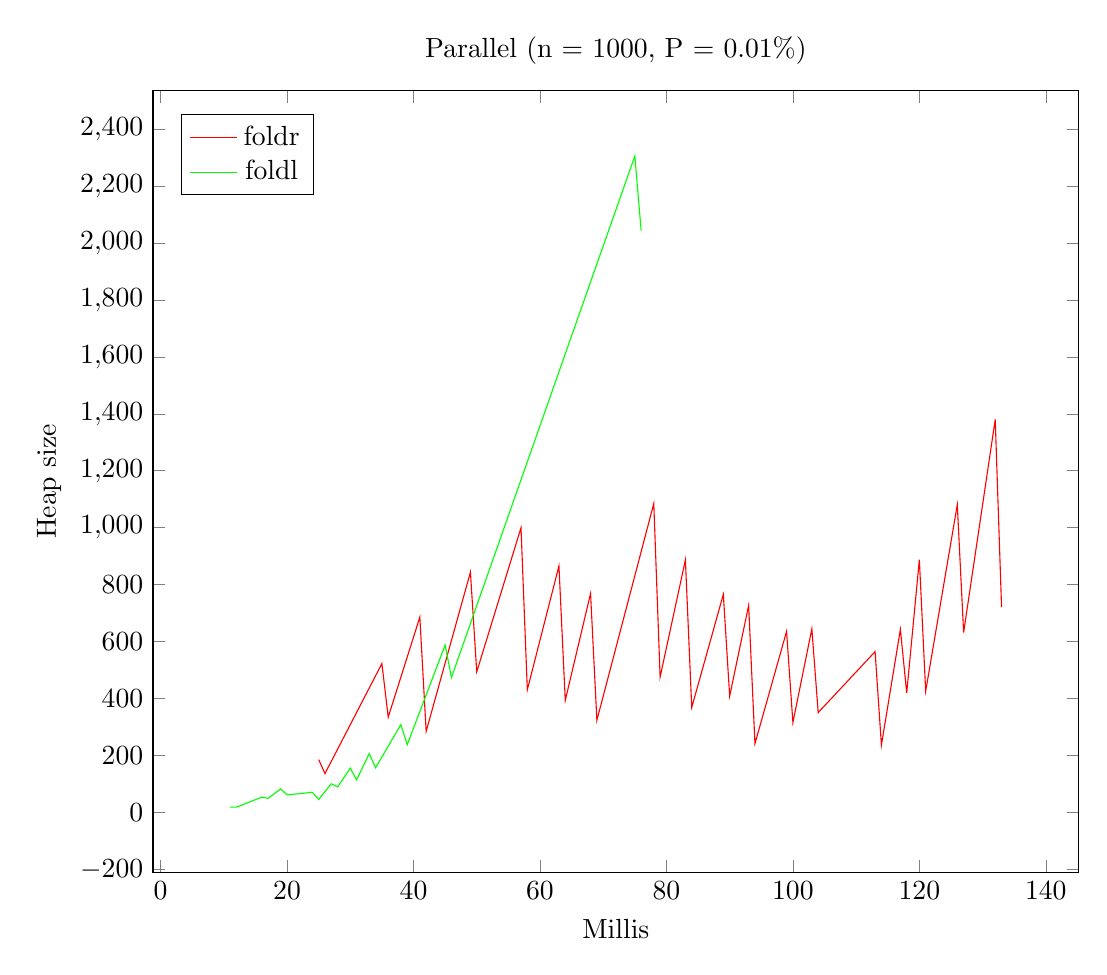
\begin{tikzpicture}
			\begin{axis}[
          title={Parallel (n = 1000, P = $0.01\%$)},
					legend pos= north west,
					width=1.1\textwidth,
					xlabel={Millis},
					ylabel={Heap size}
				]
				\addplot[
					color=red,
					%mark=square
				]
				coordinates {
(25, 186) (26, 137)
(35, 523) (36, 335)
(41, 686) (42, 285)
(49, 844) (50, 494)
(57, 1000) (58, 431)
(63, 866) (64, 394)
(68, 769) (69, 324)
(78, 1085) (79, 476)
(83, 887) (84, 369)
(89, 766) (90, 409)
(93, 727) (94, 242)
(99, 636) (100, 316)
(103, 645) (104, 351)
(113, 565) (114, 237)
(117, 643) (118, 420)
(120, 888) (121, 426)
(126, 1081) (127, 632)
(132, 1380) (133, 721)
					};
				\addlegendentry{foldr}

				\addplot[
					color=green,
					%mark=triangle
				]
				coordinates {
(11, 19) (12, 19)
(16, 54) (17, 50)
(19, 83) (20, 62)
(24, 71) (25, 46)
(27, 101) (28, 90)
(30, 156) (31, 115)
(33, 207) (34, 157)
(38, 309) (39, 238)
(45, 588) (46, 474)
(75, 2305) (76, 2043)
					};
				\addlegendentry{foldl}
			\end{axis}
		\end{tikzpicture}
		%\caption{Fibonacci function time without trimming (no trimming)}
		%\label{fig:cps:benchmark1}
	\end{subfigure}
	\hfil
	\begin{subfigure}{0.49\textwidth}
		\centering
		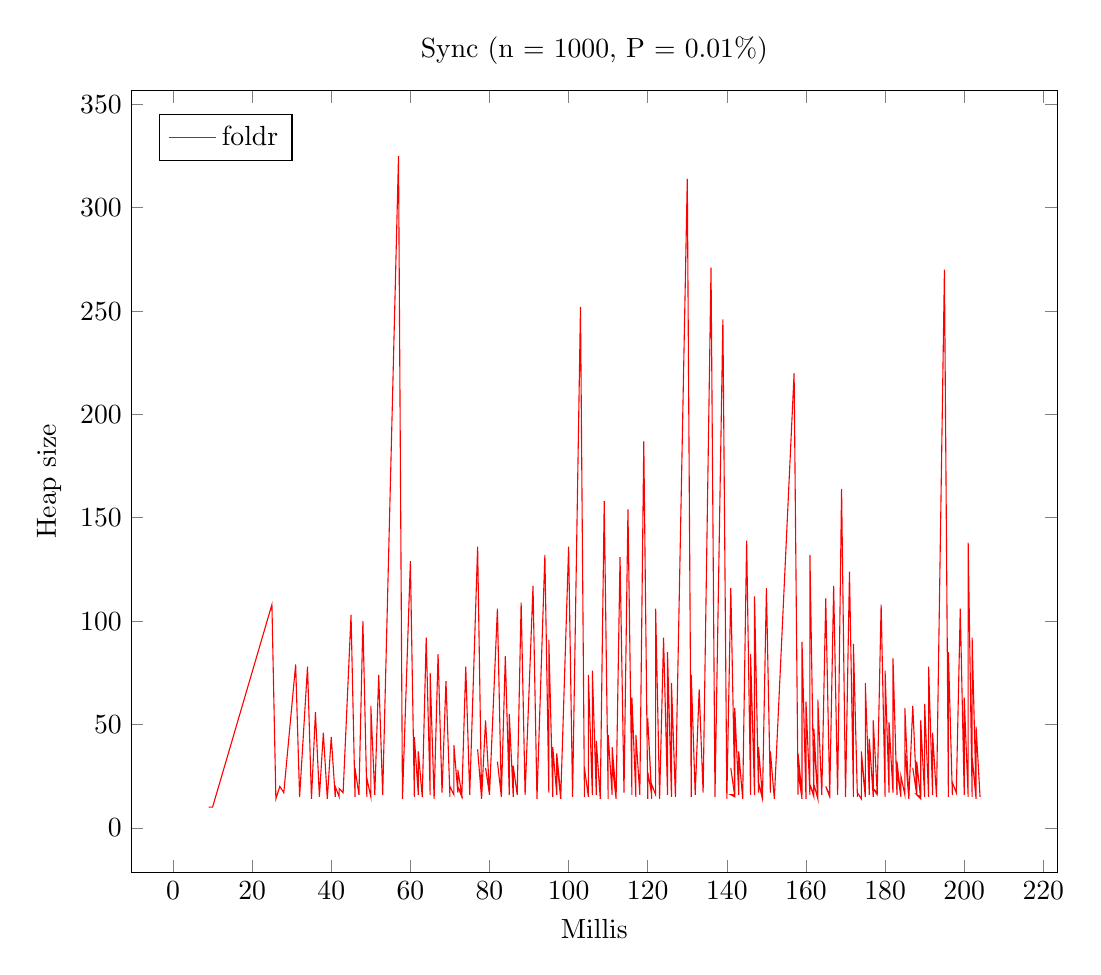
\begin{tikzpicture}
			\begin{axis}[
					title={Sync (n = 1000, P = $0.01\%$)},
					legend pos= north west,
					width=1.1\textwidth,
					xlabel={Millis},
					ylabel={Heap size}
				]
				\addplot[
					color=red,
					%mark=square
				]
				coordinates {
(9, 10) (10, 10)
(25, 108) (26, 14)
(27, 20) (28, 17)
(31, 79) (32, 15)
(34, 78) (35, 14)
(36, 56) (37, 15)
(38, 46) (39, 14)
(40, 44) (41, 15)
(41, 20) (42, 15)
(42, 19) (43, 17)
(45, 103) (46, 15)
(46, 29) (47, 16)
(48, 100) (49, 15)
(49, 24) (50, 15)
(50, 59) (51, 16)
(52, 74) (53, 16)
(57, 325) (58, 14)
(60, 129) (61, 15)
(61, 44) (62, 16)
(62, 37) (63, 15)
(64, 92) (65, 16)
(65, 75) (66, 14)
(67, 84) (68, 17)
(69, 71) (70, 15)
(70, 20) (71, 16)
(71, 40) (72, 17)
(72, 28) (73, 16)
(72, 20) (73, 15)
(74, 78) (75, 16)
(77, 136) (78, 14)
(77, 38) (78, 14)
(79, 52) (80, 17)
(79, 29) (80, 16)
(82, 106) (83, 15)
(82, 32) (83, 15)
(84, 83) (85, 16)
(85, 55) (86, 15)
(86, 30) (87, 16)
(88, 109) (89, 16)
(91, 117) (92, 14)
(94, 132) (95, 17)
(95, 91) (96, 15)
(96, 39) (97, 16)
(97, 36) (98, 16)
(97, 33) (98, 14)
(100, 136) (101, 15)
(103, 252) (104, 15)
(104, 29) (105, 15)
(105, 74) (106, 16)
(106, 76) (107, 16)
(107, 42) (108, 14)
(109, 158) (110, 14)
(110, 45) (111, 16)
(111, 39) (112, 16)
(111, 31) (112, 14)
(113, 131) (114, 17)
(115, 154) (116, 16)
(116, 63) (117, 15)
(117, 45) (118, 16)
(119, 187) (120, 14)
(120, 27) (121, 16)
(120, 53) (121, 14)
(121, 21) (122, 16)
(122, 106) (123, 14)
(124, 92) (125, 16)
(125, 85) (126, 15)
(126, 70) (127, 15)
(130, 314) (131, 15)
(131, 74) (132, 16)
(133, 67) (134, 17)
(136, 271) (137, 15)
(139, 246) (140, 14)
(141, 116) (142, 16)
(141, 16) (142, 15)
(141, 29) (142, 15)
(142, 58) (143, 16)
(143, 37) (144, 14)
(145, 139) (146, 16)
(146, 84) (147, 16)
(147, 112) (148, 17)
(148, 39) (149, 15)
(148, 22) (149, 14)
(150, 116) (151, 17)
(151, 37) (152, 14)
(157, 220) (158, 16)
(158, 35) (159, 14)
(158, 27) (159, 16)
(158, 36) (159, 16)
(159, 90) (160, 14)
(160, 61) (161, 16)
(161, 132) (162, 15)
(161, 21) (162, 16)
(162, 42) (163, 14)
(162, 48) (163, 14)
(162, 21) (163, 14)
(163, 62) (164, 16)
(165, 111) (166, 16)
(165, 20) (166, 15)
(167, 117) (168, 16)
(169, 164) (170, 15)
(171, 124) (172, 15)
(172, 89) (173, 15)
(173, 17) (174, 14)
(174, 37) (175, 16)
(174, 34) (175, 15)
(175, 70) (176, 16)
(176, 43) (177, 15)
(177, 52) (178, 17)
(177, 19) (178, 16)
(179, 108) (180, 15)
(180, 76) (181, 17)
(181, 51) (182, 17)
(182, 82) (183, 16)
(183, 32) (184, 15)
(183, 28) (184, 16)
(184, 25) (185, 16)
(185, 58) (186, 14)
(185, 38) (186, 14)
(187, 59) (188, 16)
(187, 29) (188, 16)
(188, 32) (189, 14)
(188, 16) (189, 15)
(189, 52) (190, 15)
(190, 60) (191, 15)
(191, 78) (192, 16)
(192, 46) (193, 15)
(195, 270) (196, 15)
(196, 85) (197, 16)
(197, 22) (198, 17)
(199, 106) (200, 16)
(200, 63) (201, 15)
(201, 138) (202, 15)
(202, 92) (203, 16)
(202, 34) (203, 14)
(203, 49) (204, 15)
					};
				\addlegendentry{foldr}
				%\addplot[
					%color=red,
					%mark=halfcircle*
				%]
				%coordinates {
						%(10,39)  (20,130)  (25,11010) (30,770124)
					%};
				%\addlegendentry{parallel}
			\end{axis}
		\end{tikzpicture}
		%\caption{Fibonacci sequence heap size on program termination (no trimming)}
		%\label{fig:cps:benchmark2}
	\end{subfigure}
	\begin{subfigure}{1\textwidth}
		\centering
		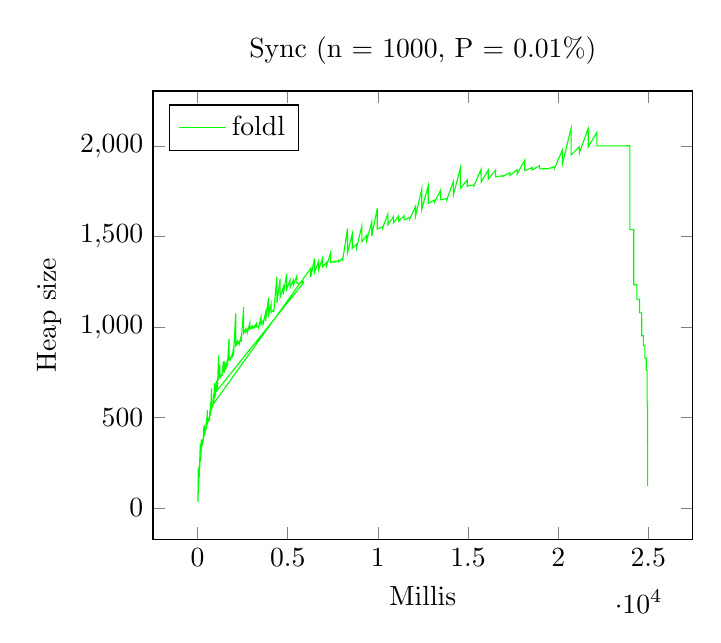
\begin{tikzpicture}
			\begin{axis}[
					title={Sync (n = 1000, P = $0.01\%$)},
					legend pos= north west,
					%width=1.1\textwidth,
					xlabel={Millis},
					ylabel={Heap size}
				]
        \addplot[
          color=green,
          %mark=triangle
        ]
        coordinates {
(22, 91) (23, 33)
(36, 217) (37, 80)
(41, 99) (42, 83)
(46, 123) (47, 94)
(49, 99) (50, 94)
(55, 188) (56, 116)
(61, 147) (62, 124)
(73, 230) (74, 151)
(82, 212) (83, 167)
(89, 194) (90, 174)
(95, 212) (96, 181)
(103, 235) (104, 195)
(112, 227) (113, 203)
(123, 275) (124, 221)
(142, 352) (143, 254)
(152, 273) (153, 257)
(163, 309) (164, 270)
(174, 290) (175, 275)
(188, 357) (189, 295)
(203, 378) (204, 316)
(219, 367) (220, 327)
(237, 377) (238, 339)
(256, 365) (257, 346)
(275, 371) (276, 352)
(291, 367) (292, 355)
(308, 372) (309, 360)
(327, 423) (328, 375)
(349, 455) (350, 395)
(372, 456) (373, 411)
(396, 435) (397, 416)
(421, 436) (422, 420)
(447, 430) (448, 423)
(476, 473) (477, 435)
(508, 498) (509, 451)
(544, 540) (545, 473)
(576, 482) (577, 475)
(608, 483) (609, 477)
(643, 498) (644, 482)
(679, 531) (680, 494)
(721, 580) (722, 515)
(772, 660) (773, 551)
(809, 574) (810, 557)
(846, 570) (847, 559)
(889, 625) (890, 576)
(938, 689) (939, 604)
(988, 675) (989, 621)
(1041, 701) (1042, 641)
(1097, 711) (1098, 660)
(1166, 842) (1167, 704)
(1231, 787) (1232, 725)
(1293, 733) (1294, 726)
(1356, 737) (1357, 729)
(1429, 810) (1430, 748)
(1505, 809) (1506, 762)
(1575, 786) (1576, 768)
(1651, 816) (1652, 781)
(1741, 934) (1742, 819)
(1822, 829) (1823, 821)
(1906, 844) (1907, 827)
(1993, 884) (1994, 841)
(2115, 1075) (2116, 899)
(2215, 922) (2216, 904)
(2319, 920) (2320, 910)
(2419, 948) (2420, 918)
(2554, 1109) (2555, 965)
(2669, 989) (2670, 971)
(2782, 989) (2783, 976)
(2901, 1023) (2902, 987)
(3024, 1005) (3025, 992)
(3145, 1004) (3146, 995)
(3261, 1018) (3262, 1000)
(3382, 1002) (3383, 1000)
(3515, 1053) (3516, 1013)
(3640, 1033) (3641, 1018)
(3776, 1080) (3777, 1033)
(3932, 1161) (3933, 1066)
(4078, 1125) (4079, 1079)
(4225, 1095) (4226, 1083)
(4400, 1278) (4401, 1131)
(4581, 1266) (4582, 1165)
(4758, 1221) (4759, 1180)
(4940, 1294) (4941, 1208)
(5133, 1259) (5134, 1219)
(5310, 1258) (5311, 1229)
(5507, 1282) (5508, 1241)
(5683, 1241) (5684, 1241)
(5875, 1251) (5876, 1244)
(889, 625) (890, 576)
(6274, 1323) (6275, 1274)
(6482, 1378) (6483, 1300)
(6709, 1362) (6710, 1314)
(6927, 1380) (6928, 1331)
(7148, 1355) (7149, 1337)
(7376, 1409) (7377, 1355)
(7591, 1363) (7592, 1357)
(7823, 1367) (7824, 1360)
(8043, 1380) (8044, 1365)
(8314, 1544) (8315, 1409)
(8576, 1512) (8577, 1434)
(8826, 1458) (8827, 1440)
(9113, 1557) (9114, 1470)
(9380, 1506) (9381, 1477)
(9658, 1580) (9659, 1502)
(9964, 1654) (9965, 1541)
(10253, 1553) (10254, 1544)
(10558, 1625) (10559, 1564)
(10860, 1609) (10861, 1574)
(11154, 1613) (11155, 1584)
(11454, 1614) (11455, 1591)
(11765, 1605) (11766, 1596)
(12087, 1665) (12088, 1611)
(12433, 1761) (12434, 1650)
(12794, 1780) (12795, 1682)
(13132, 1700) (13133, 1686)
(13482, 1756) (13483, 1702)
(13821, 1709) (13822, 1703)
(14186, 1802) (14187, 1728)
(14577, 1879) (14578, 1765)
(14956, 1812) (14957, 1777)
(15326, 1784) (15327, 1779)
(15722, 1870) (15723, 1800)
(16122, 1866) (16123, 1816)
(16528, 1865) (16529, 1829)
(16920, 1835) (16921, 1831)
(17320, 1852) (17321, 1836)
(17720, 1869) (17721, 1844)
(18148, 1922) (18149, 1863)
(18560, 1880) (18561, 1867)
(18972, 1891) (18973, 1873)
(19386, 1874) (19387, 1873)
(19797, 1884) (19798, 1876)
(20236, 1978) (20237, 1901)
(20714, 2097) (20715, 1950)
(21179, 1995) (21180, 1962)
(21665, 2096) (21666, 1994)
(22148, 2075) (22149, 2000)
(22637, 2000) (22638, 2000)
(23126, 2000) (23127, 2000)
(23630, 2000) (23631, 2000)
(23976, 2001) (23977, 1537)
(24193, 1537) (24194, 1233)
(24364, 1233) (24365, 1153)
(24509, 1153) (24510, 1077)
(24632, 1077) (24633, 951)
(24727, 951) (24728, 897)
(24811, 897) (24812, 827)
(24883, 827) (24884, 763)
(24932, 763) (24933, 585)
(24953, 585) (24954, 350)
(24960, 350) (24961, 207)
(24963, 207) (24964, 121)
          };
        \addlegendentry{foldl}

				%\addplot[
					%color=red,
					%mark=halfcircle*
				%]
				%coordinates {
						%(10,39)  (20,130)  (25,11010) (30,770124)
					%};
				%\addlegendentry{parallel}
			\end{axis}
		\end{tikzpicture}
		%\caption{Fibonacci sequence heap size on program termination (no trimming)}
		%\label{fig:cps:benchmark2}
	\end{subfigure}
  \caption{}
  \label{fig:foldcomp}
\end{figure}
%\begin{remark}
%If the program is to remain within a constant amount of space throughout the evaluation of \texttt{foldl}, then garbage collection must support this choice.
%Clearly a simple strategy 
%\end{remark}

%\\
%\begin{minipage}{\textwidth}
%\begin{lemma}
%\texttt{mapTail} is tail recursive and requires an additional $O(n \cdot m)$ space when evaluated on a list of size $n$ with a function \texttt{f} produces values of size $m$.
%\end{lemma}
%\begin{proof}
%Unpacking \texttt{Cons} and \texttt{Nil} as their underlying scott encoded functions is omitted for readability.
%In this proof the list is of \texttt{Int} and \texttt{f} is the identity function.
%For some $1 \leq k \leq n$ where $n$ is the size of the list, at the recursive invocation of \texttt{mapImpl}, the list is partitioned into the lower $1, \dots k - 1$ elements (\texttt{b (Cons x)}) and the higher $k, \dots n$ elements (\texttt{xs}).
%\begin{align}
%&\texttt{ mapTail (Cons 1 (Cons 2 $\dots$ (Cons n Nil))) ($\lambda$x.x)}  \\
%=&\texttt{ r Nil ($\lambda$x.$\lambda$xs.mapImpl xs ($\lambda$x.x) (Cons (f x)))}  \tag*{} \\
%=&\texttt{ mapImpl (Cons 2 (Cons 3 $\dots$ (Cons n Nil))) ($\lambda$x.x) (Cons 1)}  \eqtag{2$\dots$n} \label{eq:map:2n} \\
%=&\texttt{ r (b Nil) ($\lambda$x.$\lambda$xs.mapImpl xs f (b (Cons (f x))))}  \tag*{} \\
%=&\texttt{ mapImpl xs f (($\lambda$xs.Cons 1 xs) (Cons 2))}  \tag*{} \\
%=&\texttt{ mapImpl xs f (($\lambda$xs.Cons 1 xs) (Cons 2))}  \tag*{} \\
%=&\texttt{ mapImpl xs f (Cons 1 (Cons 2))}  \tag*{} \\
%=&\texttt{ mapImpl (Cons 3 (Cons 4 $\dots$ (Cons n Nil))) ($\lambda$x.x) (Cons 1 (Cons 2))}  \eqtag{3$\dots$n} \label{eq:map:3n} \\
%=&\texttt{ r (b Nil) ($\lambda$x.$\lambda$xs.mapImpl xs f (b (Cons (f x))))}  \tag*{} \\
%=&\texttt{ mapImpl xs f (($\lambda$xs.Cons 1 (Cons 2 xs)) (Cons 3))}  \tag*{} \\
%=&\texttt{ mapImpl (Cons 4 (Cons 5 $\dots$ (Cons n Nil))) ($\lambda$x.x) (Cons 1 (Cons 2 (Cons 3)))}  \eqtag{4$\dots$n} \\
%=&\dots\tag*{}\\
%=&\texttt{ mapImpl (Cons k (Cons (k + 1) $\dots$ (Cons n Nil)))} \tag*{} \\
%&\texttt{ ($\lambda$x.x) (Cons 1 ($\dots$ (Cons (k - 1))))}  \tag*{} 
%\end{align}
%The base case for the proof is once \texttt{mapImpl} is recursively invoked (\autoref{eq:map:2n}), size of the newly created list is $m \cdot 1$ (\texttt{f (Cons 1)}).
%The first recursive iteration for \texttt{mapImpl} is the step between \autoref{eq:map:2n} and \autoref{eq:map:3n} such that the size becomes $m \cdot 2$ (\texttt{Cons (f 1) (Cons (f 2))}).
%If we assume that the first $k$ recursive iterations have size $m \cdot k$, then the $k+1$'th iteration has size $m \cdot (k + 1)$ by \texttt{Cons (f 1) (Cons (f 2) $\dots$ (Cons (f (k + 1))))}.
%Clearly whet $k = n$ then the newly created list is of size $m \cdot n$ and \texttt{xs} is empty, thus the function is.
%\end{proof}
%\end{minipage}

%When evaluating a term that results in a change to the substitution mapping the previous substitution mapping version is paired with it.
%Letting the substitution mapping be 
%$\{ \texttt{x} \mapsto (\lambda \texttt{x.g x}, \{ \texttt{g} \mapsto (\lambda \texttt{x.x}, \emptyset)) \}, \texttt{g} \mapsto (\lambda \texttt{x.x}, \emptyset)\}$
%the space complexity may seem to grow by $O(n^3)$ (\autoref{eq:evalruntimewrong}) but lifting the data structure to using pointers instead of copies reduces the size to $O(n)$.
%\begin{align}
%\label{eq:evalruntimewrong}
%& O \left( \sum_{k = 1}^n \sum_{i = 1}^{k} i \right) \\
%= \,\,\, & O \left( \sum_{k = 1}^n \frac{k(k + 1)}{2}\right)\tag{Triangular}\\
%= \,\,\,& O \left( \frac{1}{2} \left( \sum_{k = 1}^n k^2 + \sum_{k = 1} k \right) \right)\tag*{}\\
%= \,\,\,& O \left( \sum_{k = 1}^n k^2 \right)\tag*{}\\
%= \,\,\,& O \left( \frac{1}{6}n + \frac{1}{2}n^2 + \frac{1}{3}n^3 \right)\tag{Faulhaber}\\
%= \,\,\,& O \left( n^3 \right)\tag*{}
%\end{align}
%Observe that the introduction of a context is based on free variables in closures and can in fact be avoided at the cost of compilation time by simply making all variables unique.
%Let \autoref{eq:eval:comp} be a program translated from \autoref{eq:eval:nocomp}.
%\begin{align}
%&(\lambda x . \texttt{ let } f = \lambda y . \lambda x . x \texttt{ in } x) \label{eq:eval:nocomp}\\
%&(\lambda x_1 . \texttt{ let } x_2 = \lambda x_3 . \lambda x_4 . x_4 \texttt{ in } x_1)\label{eq:eval:comp}
%\end{align}
%The method of storing substitutions warrants the question of evaluation strategy since eagerly replacing the mapped to expressions implies call by value (\autoref{eq:eval:eagereval}).
%If one were to keep the initially proposed semantics the result would be call by name (\autoref{eq:eval:name}).
%In the hybrid approach forcing a term rewrites the mapped to value (\autoref{eq:eval:need}).
%\begin{align}
%&\{ \texttt{x} \mapsto \texttt{y} \} \cdot \{ \texttt{y} \mapsto 5 \} \rightarrow \{ \texttt{x} \mapsto 5, \texttt{y} \mapsto 5 \} \label{eq:eval:eagereval} \eqtag{Call by value}\\
%&\{ \texttt{x} \mapsto \texttt{y} \} \cdot \{ \texttt{y} \mapsto 5 \} \rightarrow \{ \texttt{x} \mapsto \texttt{y}, \texttt{y} \mapsto 5 \} \label{eq:eval:name} \eqtag{Call by name}\\
%&\textit{force}(\texttt{z}, \{ \texttt{f} \mapsto \lambda \texttt{x.x}, \texttt{z} \mapsto \texttt{f 0} \}) = \{ \texttt{f} \mapsto \lambda \texttt{x.x}, \texttt{z} \mapsto 0 \} \label{eq:eval:need} \eqtag{Call by need}
%\end{align}
%One may also have an interpreter that supports multiple strategies at once by simply specifying what type of strategy should be applied to every term.
%Evaluating a program is a matter of entering through some expression and continually reading terms and applying substitutions until said expression has been evaluated regardless of evaluation strategy. 

%The algorithm for evaluating the untyped lambda calculus is similar to Algorithm W (\autoref{fig:dmrules}) and can be seen in.
%\begin{figure}[ht]
%\begin{mdframed}[style=style1]
%\vspace*{0.4cm}
%\begin{subfigure}[b]{0.30\textwidth}
%\begin{prooftree}
%\AxiomC{$e$}
%\RightLabel{Terminal}
%\UnaryInfC{$\emptyset ,e$}
%\end{prooftree}   
%\label{eq:prooftree:terminal}
%\caption{}
%\end{subfigure}
%\begin{subfigure}[b]{0.69\textwidth}
%\begin{prooftree}
%\AxiomC{$S,\lambda x . e_1$}
%\AxiomC{$S \cdot \{ x \mapsto e_2 \},e_1 $}
%\RightLabel{App}
%\BinaryInfC{$S,e_3$}
%\end{prooftree}   
%\label{eq:prooftree:ref}
%\caption{}
%\end{subfigure}
%\begin{subfigure}[b]{1\textwidth}
%\begin{prooftree}
%\AxiomC{$S \cdot \{ x \mapsto e_1 \},e_2$}
%\RightLabel{Let}
%\UnaryInfC{$S,\texttt{ let } x = e_1 \texttt{ in } e_2$}
%\end{prooftree}   
%\label{eq:prooftree:ref}
%\caption{}
%\end{subfigure}

%\end{mdframed}

%\end{figure}

%Consider the De Bruijn form of \autoref{lst:add} where \texttt{2} is the index of \texttt{a} and \texttt{1} is the index of \texttt{b}.
%Beta reductions with De Bruijn indices~\cite{de1972lambda} is another more straightforward method of evaluating the untyped lambda calculus.
%De Bruijn indices is a representation of lambda calculus which deals with variables based on the scope ''distance`` instead of variable names.
%\begin{lstlisting}[language=ML,caption={Add as De Bruijn},label={lst:adddebru},mathescape=true]
%let add = ($\lambda$($\lambda$ 2 1))
%\end{lstlisting}
%Consider the De Bruijn form of \autoref{lst:add} where \texttt{2} is the index of \texttt{a} and \texttt{1} is the index of \texttt{b}.
%More generally all variable occurrences are replaced with the distance to the abstraction which introduced them.
%The use of De Bruijn indices allow anonymous naming of parameters thus imply a method of solving the application problem when directly interpreting the untyped lambda calculus.
%A minor but important detail when 
%\begin{align}
%&(\lambda x . ((\lambda f. \lambda x. f x)(\lambda z . z))x)''0`` \rightarrow\\
%&
%\end{align}

